\documentclass[]{ctexbook}
\usepackage{lmodern}
\usepackage{amssymb,amsmath}
\usepackage{ifxetex,ifluatex}
\usepackage{fixltx2e} % provides \textsubscript
\ifnum 0\ifxetex 1\fi\ifluatex 1\fi=0 % if pdftex
  \usepackage[T1]{fontenc}
  \usepackage[utf8]{inputenc}
\else % if luatex or xelatex
  \ifxetex
    \usepackage{xltxtra,xunicode}
  \else
    \usepackage{fontspec}
  \fi
  \defaultfontfeatures{Ligatures=TeX,Scale=MatchLowercase}
\fi
% use upquote if available, for straight quotes in verbatim environments
\IfFileExists{upquote.sty}{\usepackage{upquote}}{}
% use microtype if available
\IfFileExists{microtype.sty}{%
\usepackage{microtype}
\UseMicrotypeSet[protrusion]{basicmath} % disable protrusion for tt fonts
}{}
\usepackage[b5paper,tmargin=2.5cm,bmargin=2.5cm,lmargin=3.5cm,rmargin=2.5cm]{geometry}
\usepackage[unicode=true]{hyperref}
\PassOptionsToPackage{usenames,dvipsnames}{color} % color is loaded by hyperref
\hypersetup{
            pdftitle={rBAS使用文档},
            pdfauthor={王江宇},
            colorlinks=true,
            linkcolor=Maroon,
            citecolor=Blue,
            urlcolor=Blue,
            breaklinks=true}
\urlstyle{same}  % don't use monospace font for urls
\usepackage{natbib}
\bibliographystyle{apalike}
\usepackage{color}
\usepackage{fancyvrb}
\newcommand{\VerbBar}{|}
\newcommand{\VERB}{\Verb[commandchars=\\\{\}]}
\DefineVerbatimEnvironment{Highlighting}{Verbatim}{commandchars=\\\{\}}
% Add ',fontsize=\small' for more characters per line
\usepackage{framed}
\definecolor{shadecolor}{RGB}{248,248,248}
\newenvironment{Shaded}{\begin{snugshade}}{\end{snugshade}}
\newcommand{\KeywordTok}[1]{\textcolor[rgb]{0.13,0.29,0.53}{\textbf{#1}}}
\newcommand{\DataTypeTok}[1]{\textcolor[rgb]{0.13,0.29,0.53}{#1}}
\newcommand{\DecValTok}[1]{\textcolor[rgb]{0.00,0.00,0.81}{#1}}
\newcommand{\BaseNTok}[1]{\textcolor[rgb]{0.00,0.00,0.81}{#1}}
\newcommand{\FloatTok}[1]{\textcolor[rgb]{0.00,0.00,0.81}{#1}}
\newcommand{\ConstantTok}[1]{\textcolor[rgb]{0.00,0.00,0.00}{#1}}
\newcommand{\CharTok}[1]{\textcolor[rgb]{0.31,0.60,0.02}{#1}}
\newcommand{\SpecialCharTok}[1]{\textcolor[rgb]{0.00,0.00,0.00}{#1}}
\newcommand{\StringTok}[1]{\textcolor[rgb]{0.31,0.60,0.02}{#1}}
\newcommand{\VerbatimStringTok}[1]{\textcolor[rgb]{0.31,0.60,0.02}{#1}}
\newcommand{\SpecialStringTok}[1]{\textcolor[rgb]{0.31,0.60,0.02}{#1}}
\newcommand{\ImportTok}[1]{#1}
\newcommand{\CommentTok}[1]{\textcolor[rgb]{0.56,0.35,0.01}{\textit{#1}}}
\newcommand{\DocumentationTok}[1]{\textcolor[rgb]{0.56,0.35,0.01}{\textbf{\textit{#1}}}}
\newcommand{\AnnotationTok}[1]{\textcolor[rgb]{0.56,0.35,0.01}{\textbf{\textit{#1}}}}
\newcommand{\CommentVarTok}[1]{\textcolor[rgb]{0.56,0.35,0.01}{\textbf{\textit{#1}}}}
\newcommand{\OtherTok}[1]{\textcolor[rgb]{0.56,0.35,0.01}{#1}}
\newcommand{\FunctionTok}[1]{\textcolor[rgb]{0.00,0.00,0.00}{#1}}
\newcommand{\VariableTok}[1]{\textcolor[rgb]{0.00,0.00,0.00}{#1}}
\newcommand{\ControlFlowTok}[1]{\textcolor[rgb]{0.13,0.29,0.53}{\textbf{#1}}}
\newcommand{\OperatorTok}[1]{\textcolor[rgb]{0.81,0.36,0.00}{\textbf{#1}}}
\newcommand{\BuiltInTok}[1]{#1}
\newcommand{\ExtensionTok}[1]{#1}
\newcommand{\PreprocessorTok}[1]{\textcolor[rgb]{0.56,0.35,0.01}{\textit{#1}}}
\newcommand{\AttributeTok}[1]{\textcolor[rgb]{0.77,0.63,0.00}{#1}}
\newcommand{\RegionMarkerTok}[1]{#1}
\newcommand{\InformationTok}[1]{\textcolor[rgb]{0.56,0.35,0.01}{\textbf{\textit{#1}}}}
\newcommand{\WarningTok}[1]{\textcolor[rgb]{0.56,0.35,0.01}{\textbf{\textit{#1}}}}
\newcommand{\AlertTok}[1]{\textcolor[rgb]{0.94,0.16,0.16}{#1}}
\newcommand{\ErrorTok}[1]{\textcolor[rgb]{0.64,0.00,0.00}{\textbf{#1}}}
\newcommand{\NormalTok}[1]{#1}
\usepackage{longtable,booktabs}
% Fix footnotes in tables (requires footnote package)
\IfFileExists{footnote.sty}{\usepackage{footnote}\makesavenoteenv{long table}}{}
\usepackage[normalem]{ulem}
% avoid problems with \sout in headers with hyperref:
\pdfstringdefDisableCommands{\renewcommand{\sout}{}}
\IfFileExists{parskip.sty}{%
\usepackage{parskip}
}{% else
\setlength{\parindent}{0pt}
\setlength{\parskip}{6pt plus 2pt minus 1pt}
}
\setlength{\emergencystretch}{3em}  % prevent overfull lines
\providecommand{\tightlist}{%
  \setlength{\itemsep}{0pt}\setlength{\parskip}{0pt}}
\setcounter{secnumdepth}{5}
% Redefines (sub)paragraphs to behave more like sections
\ifx\paragraph\undefined\else
\let\oldparagraph\paragraph
\renewcommand{\paragraph}[1]{\oldparagraph{#1}\mbox{}}
\fi
\ifx\subparagraph\undefined\else
\let\oldsubparagraph\subparagraph
\renewcommand{\subparagraph}[1]{\oldsubparagraph{#1}\mbox{}}
\fi

% set default figure placement to htbp
\makeatletter
\def\fps@figure{htbp}
\makeatother

\usepackage{booktabs}
\usepackage{longtable}

\usepackage{framed,color}
\definecolor{shadecolor}{RGB}{248,248,248}

\renewcommand{\textfraction}{0.05}
\renewcommand{\topfraction}{0.8}
\renewcommand{\bottomfraction}{0.8}
\renewcommand{\floatpagefraction}{0.75}

\let\oldhref\href
\renewcommand{\href}[2]{#2\footnote{\url{#1}}}

\makeatletter
\newenvironment{kframe}{%
\medskip{}
\setlength{\fboxsep}{.8em}
 \def\at@end@of@kframe{}%
 \ifinner\ifhmode%
  \def\at@end@of@kframe{\end{minipage}}%
  \begin{minipage}{\columnwidth}%
 \fi\fi%
 \def\FrameCommand##1{\hskip\@totalleftmargin \hskip-\fboxsep
 \colorbox{shadecolor}{##1}\hskip-\fboxsep
     % There is no \\@totalrightmargin, so:
     \hskip-\linewidth \hskip-\@totalleftmargin \hskip\columnwidth}%
 \MakeFramed {\advance\hsize-\width
   \@totalleftmargin\z@ \linewidth\hsize
   \@setminipage}}%
 {\par\unskip\endMakeFramed%
 \at@end@of@kframe}
\makeatother

\makeatletter
\@ifundefined{Shaded}{
}{\renewenvironment{Shaded}{\begin{kframe}}{\end{kframe}}}
\@ifpackageloaded{fanyverb}{%
  % https://github.com/CTeX-org/ctex-kit/issues/331
  \RecustomVerbatimEnvironment{Highlighting}{Verbatim}{commandchars=\\\{\},formatcom=\xeCJKVerbAddon}%
}{}
\makeatother

\usepackage{makeidx}
\makeindex

\urlstyle{tt}

\usepackage{amsthm}
\makeatletter
\def\thm@space@setup{%
  \thm@preskip=8pt plus 2pt minus 4pt
  \thm@postskip=\thm@preskip
}

\makeatother

\makeatletter
\def\CTEX@section@format{\Large\bfseries\flushleft}
\makeatother

\frontmatter

\title{rBAS使用文档}
\author{王江宇}
\date{2018-08-28}

\usepackage{amsthm}
\newtheorem{theorem}{Theorem}[chapter]
\newtheorem{lemma}{Lemma}[chapter]
\theoremstyle{definition}
\newtheorem{definition}{Definition}[chapter]
\newtheorem{corollary}{Corollary}[chapter]
\newtheorem{proposition}{Proposition}[chapter]
\theoremstyle{definition}
\newtheorem{example}{Example}[chapter]
\theoremstyle{definition}
\newtheorem{exercise}{Exercise}[chapter]
\theoremstyle{remark}
\newtheorem*{remark}{Remark}
\newtheorem*{solution}{Solution}
\let\BeginKnitrBlock\begin \let\EndKnitrBlock\end
\begin{document}
\maketitle

{
\setcounter{tocdepth}{2}
\tableofcontents
}
\listoftables
\listoffigures
\mainmatter

\chapter*{前言}


\section*{手册内容概述}


本手册是为了大家更好地使用\textbf{rBAS}\index{rBAS}
\citep{R-rBAS}包而撰写,内容如下:

\begin{itemize}
\item
  第 \ref{install}
  章介绍了如何安装\texttt{R}语言的环境,来使用\texttt{rBAS}包。不用担心,\texttt{R}的语法很简单,各种功能是按照自身的需要安装各种\texttt{packages},所以比\texttt{matlab}体积更小,入门时间成本也较低。\textbf{哪怕你无意于\texttt{R}的学习,也可以看看本手册的原理篇(第
  \ref{algorithm} 章),应用篇(第\ref{examples}章)以及后续的更新计划(第
  \ref{updates}
  章),来了解算法的原理,出现了哪些变种,以及有着什么样的工程应用}。
\item
  第 \ref{algorithm}
  章介绍了\textbf{BAS算法}以及在其基础上出现的各种\textbf{改进算法}的\textbf{原理},当然,随着算法的不断改进和发展,这个文档还需要随之不断更新。
\item
  第 \ref{rBAS}
  章讲述了如何在\texttt{R}中使用\texttt{rBAS}包\textbf{调用收录的算法的对应函数},以及一些简单的\textbf{案例}(大部分是\texttt{BAS}相关文献中的算例和\texttt{benchmark\ functions})。每一句出现的代码我都会尽我所能去注释,让大家了解每一步的意义,以及\texttt{R}的简单易用。我也希望,自己的语言能尽力通俗,对于其他工具的使用者来说。
\item
  第 \ref{examples}
  章主要介绍的是BAS及变体算法\textbf{在各种领域的应用},当然,少不了对应的案例描述和代码。\textbf{可能有些涉及到各位作者的研究,不会做到完全的开源},但在\textbf{李帅}老师的组织下,我相信这会是最完善全面的\texttt{BAS}应用大全。
\item
  第 \ref{interface} 章介绍了\texttt{rBAS}中的用户界面的调用,以及运行。
\item
  第 \ref{updates}
  章讲述了\texttt{rBAS}包的\textbf{开发和使用手册更新的计划}。因为算法总是会不断地推陈出新,所以\texttt{rBAS}包也必须和目前的研究保持一致。如果你有好的想法,可以看此章的内容,然后把自己的建议传达给我们。
\end{itemize}

\begin{quote}
好了,冗长的章节介绍完毕。大家可以开始浏览正文了。
\end{quote}

\section*{夹带私货}


如果你对这本手册本身的撰写环境感兴趣的话,那我可能还要啰嗦两句。

\emph{第一句}:照搬 \href{http://yihui.name/}{Yihui}
的一句话:我用了两个 R 包编译这本书,分别是 \textbf{knitr}\index{knitr}
\citep{xie2015} 和 \textbf{bookdown}\index{bookdown}
\citep{R-bookdown}。

\emph{第二句}:感谢
Yihui。嗯\ldots{},因为这个男人,R用户的读书笔记,文章,学位论文,个人网站等等都可以在R里面撰写或者开发。不得不感慨他的天才和对需求的把握。

\section*{致谢}


感谢提倡者\texttt{李帅}老师,以及\texttt{姜向远}博士。他们是\texttt{BAS}的提出者,也在算法原理与改进上,给了我这个做暖通的门外汉以启发。

此外,还感谢\texttt{李晓晓},\texttt{王甜甜},\texttt{莫小娟},\texttt{阮月}同学贡献自己的算法代码和应用案例,他(她)们改进了算法,并且让其应用部分变得更加丰富。

当然,还得感谢Yihui的\texttt{bookdown}。

老实讲,2018/07,也就是一个月以前,我刚开始用\texttt{R}编写这个算法,然后用在自己的建筑系统辨识研究中,没想到\(\dots\)
所以,这个手册是比较仓促的产物,再加之自身关于优化算法理论水平较低,如果大家发现了本手册的各种问题,欢迎在QQ群(437958608)内留言,或者是在\texttt{rBAS}的
github上提出 \href{https://github.com/jywang2016/rBAS/issues}{issues}。

总之,谢谢上述老师及同学,也谢谢未来给我提供问题或建议的同学,你们的帮助,让手册更加完善。

\BeginKnitrBlock{flushright}
王江宇\\
2018/08/18\\
华中科技大学
\EndKnitrBlock{flushright}

\chapter*{作者简介}\label{author}


\begin{itemize}
\tightlist
\item
  包作者

  \begin{itemize}
  \tightlist
  \item
    王江宇:
    \texttt{BSAS}算法,创建维护\texttt{rBAS}包。\href{https://github.com/jywang2016/rBAS}{Github}
  \item
    李帅:
    提出\texttt{BAS}以及\texttt{BAS-WPT}算法。\href{http://www4.comp.polyu.edu.hk/~cssli/}{个人主页}
    \&
    \href{http://scholar.google.com/citations?hl=zh-CN\&user=H8UOWqoAAAAJ}{谷歌学术}
  \item
    姜向远: 提出\texttt{BAS}以及\texttt{BAS-WPT}算法。
  \end{itemize}
\item
  贡献者

  \begin{itemize}
  \tightlist
  \item
    李晓晓: 二阶\texttt{BAS}
  \item
    王甜甜: 天牛群体优化算法\texttt{BSO}
  \item
    阮月: \texttt{Binary-BAS}
  \item
    莫小娟: 多杆机构优化问题
  \end{itemize}
\end{itemize}

\chapter{R以及rBAS安装}\label{install}

\texttt{R}以及其集成开发环境(IDE)\texttt{Rstudio}加起来都不到200M,所以大家放心下载安装,不会是需要10+G的庞然大物。当然,\texttt{matlab}也是很好的科学计算软件,这里仅仅是说明安装的大小。

总体来说,R的安装十分简单,类似于把大象装进冰箱只需要三步。

\section{R安装}\label{Rinstall}

\texttt{Step1}: 进入R的网站 \url{https://www.r-project.org/}
,然后点击左上角\texttt{Download}底下的\texttt{CRAN}。

\texttt{Step2}:
选择并点击\texttt{China}底下的镜像网址,方便下载。然后点击\texttt{Download\ R\ for\ windows},出现的界面右上角有\texttt{install\ R\ for\ the\ first\ time},点击即可下载。

\texttt{Step3}: 安装,不需要各种复杂的配置,按照给定提示操作即可。

但是,打开R,你会发现是如图\ref{fig:rface}这样过于\texttt{简洁}的界面。

\begin{figure}

{\centering 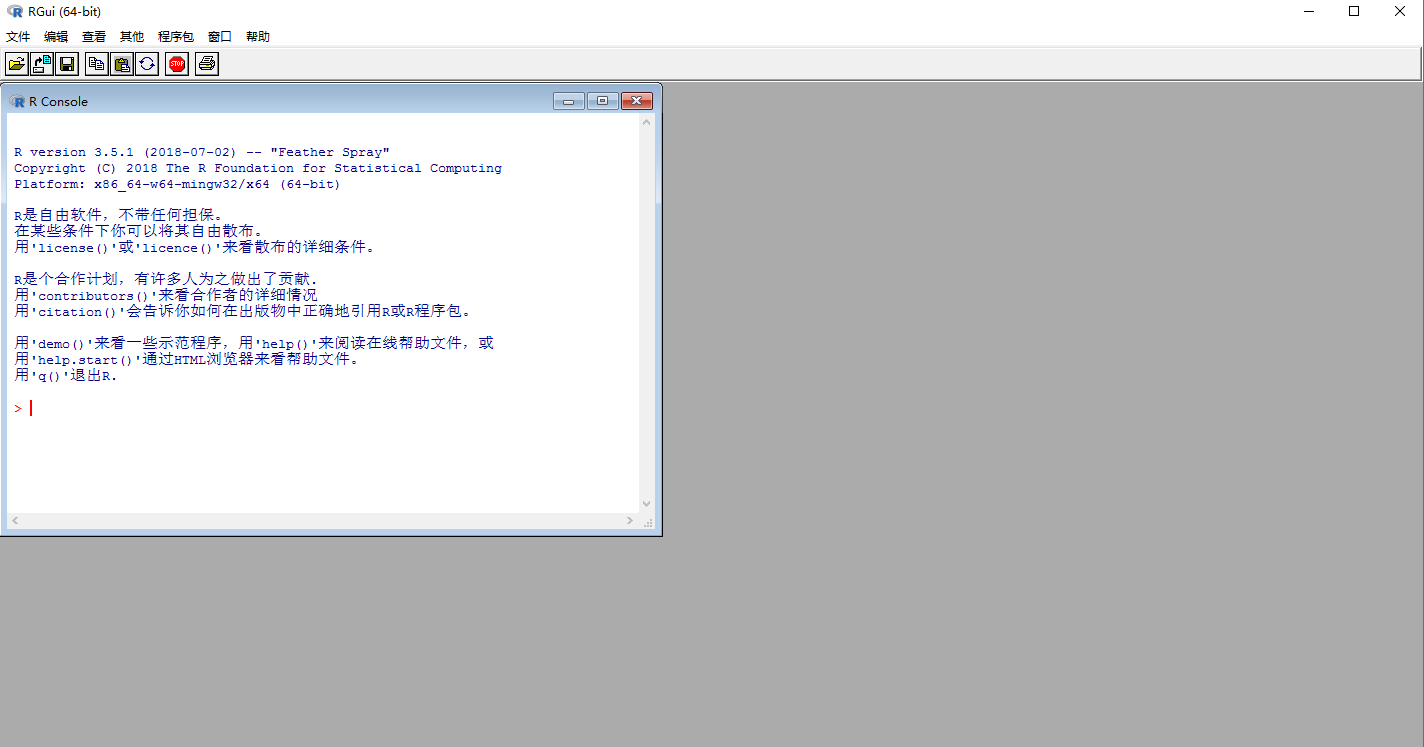
\includegraphics[width=0.8\linewidth]{img/R} 

}

\caption{R界面}\label{fig:rface}
\end{figure}

这并不符合新手的操作和开发习惯。因此,你可能需要一个集成开发环境,最好是有函数、变量的提示,方便浏览代码和结果等等优势的软件。那么,我想你说的应该是
\texttt{Rstudio}。

\section{Rstudio安装}\label{Rstudioinstall}

\texttt{Step1}: 进入下载页面
\url{https://www.rstudio.com/products/rstudio/download/} 。

\texttt{Step2}: 选择\texttt{free}版本的下载。

\texttt{Step3}: 安装,无需配置特别的环境变量等。

那么,打开\texttt{Rstudio}后,会看到如图\ref{fig:rstudioface}这样的界面。

\begin{figure}

{\centering 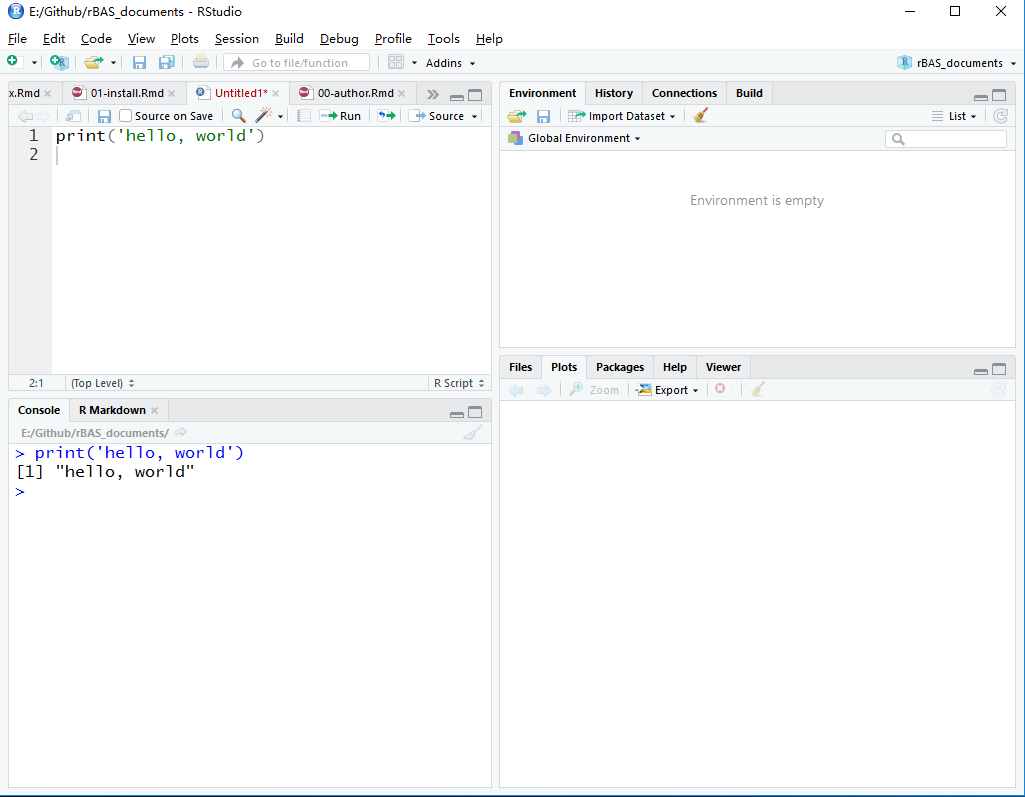
\includegraphics[width=0.8\linewidth]{img/Rstudio} 

}

\caption{Rstudio界面}\label{fig:rstudioface}
\end{figure}

左上角是撰写代码脚本的区域,左下角是结果输出的窗口。右下角的\texttt{files}可以查看工作路径下的文件,和\texttt{matlab}左侧的栏目是类似的;\texttt{plots}用于查看使用代码绘制的图像,\texttt{packages}可以用于安装\texttt{CRAN}上发布,或者是本地的\texttt{packages},也就类似\texttt{matlab}的\texttt{toolbox};\texttt{help}则是用来显示各个函数的帮助文档;\texttt{Viewer}则是用来预览\texttt{R}生成的交互图像(比如\texttt{plotly}绘制的图),生成的网页(比如我现在正在使用\texttt{bookdown}包来写本手册,那就可以预览生成的\texttt{gitbook}电子书的内容)等等。右上角的\texttt{Environment}显示被加载进来的函数,变量等信息,和\texttt{matlab}的\texttt{workspace}是类似的。
剩下的和本手册无关,可以在后面的开发中慢慢了解。

\section{rBAS安装}\label{rBASinstall}

在\texttt{Rstudio}的\texttt{Console}框内输入:

\begin{Shaded}
\begin{Highlighting}[]
\KeywordTok{install.packages}\NormalTok{(}\StringTok{'devtools'}\NormalTok{)}
\end{Highlighting}
\end{Shaded}

因为目前\texttt{rBAS}包还不在\texttt{CRAN}内,所以需要通过\texttt{devtools}包,来从\texttt{github}上安装。所以我们先在本地安装\texttt{devtools}包。如果觉得代码敲的累,那么有个更直观的方式,如图\ref{fig:devtools}:

\begin{figure}

{\centering 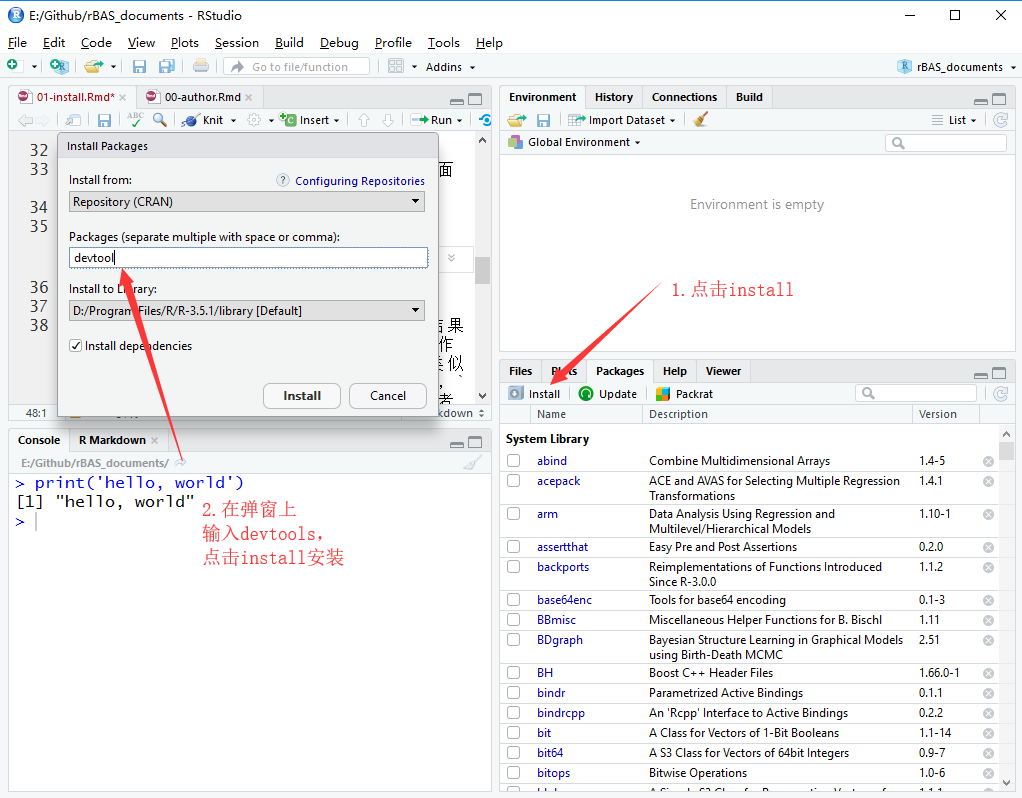
\includegraphics[width=0.8\linewidth]{img/rBAS} 

}

\caption{devtools手动安装示意图}\label{fig:devtools}
\end{figure}

最后,有了\texttt{devtools}包,我们可以从\texttt{github}上安装\texttt{rBAS}包了。

\begin{Shaded}
\begin{Highlighting}[]
\CommentTok{#不加载devtools,只调用其中的函数}
\NormalTok{devtools}\OperatorTok{::}\KeywordTok{install_github}\NormalTok{(}\StringTok{"jywang2016/rBAS"}\NormalTok{)}
\end{Highlighting}
\end{Shaded}

接下来,我们可以使用\texttt{rBAS}的函数了。

\chapter{算法原理}\label{algorithm}

本章讲述目前\texttt{rBAS}集成的三种算法的原理。如有错漏,还请指出。

\section{BAS}\label{bas}

关于\texttt{BAS},主要的参考资料为\texttt{姜向远}博士和\texttt{李帅}老师在\texttt{arXiv}上的论文,\href{https://arxiv.org/abs/1710.10724}{BAS:
beetle antennae search algorithm for optimization
problems}。而我是在知乎上看到一篇\href{https://zhuanlan.zhihu.com/p/30742461}{文章}后,才开始复现\texttt{BAS}算法。

\subsection{算法流程}\label{BASflow}

1.随机生成方向向量,标准化

\begin{equation}
\overrightarrow{\mathbf{b}}=\frac{\text{rnd}(n,1)}{\|\text{rnd}(n,1)\|}
\label{eq:dir}
\end{equation}

其中,\(n\)是待优化参数的维度。

2.计算左右须的坐标

\begin{equation}
\begin{split}
\mathbf{x}_r&=\mathbf{x}^t+d^t\overrightarrow{\mathbf{b}} \\
\mathbf{x}_l&=\mathbf{x}^t-d^t\overrightarrow{\mathbf{b}}
\end{split}
\label{eq:xlxr}
\end{equation}

其中,\(\mathbf{x}^t\)为\(t\)时刻天牛的位置,\(d^t\)则是\(t\)时刻,质心到须的距离。

3.根据两须对应函数值,决定天牛下一时刻移动位置

\begin{equation}
\mathbf{x}^t=\mathbf{x}^{t-1}+\delta^t\overrightarrow{\mathbf{b}}\text{sign}(f(\mathbf{x}_r)-f(\mathbf{x}_l))
\label{eq:xupdate}
\end{equation}

其中,\(\delta^t\)为t时刻的步长,\(f\)为待优化目标函数。

4.步长与搜索距离更新

\begin{align}
d^t&= \eta_d d^{t-1}+d_0 \label{eq:dupdate}\\
\delta^t&=\eta_{\delta} \delta^{t-1} \label{eq:deltaupdate}
\end{align}

其中,\(d_0\)是人为设定的距离的常数,\(\eta_d\)与\(\eta_\delta\)分别是搜索距离和步长的更新衰减系数。

为了避免参数过多,姜向远博士在\texttt{BAS-WPT}算法中是按照式\eqref{eq:WPTupdate}来更新搜索距离和步长的。其中,\(c_2\)是人为设定的常数。

\begin{equation}
\begin{split}
\delta^t&=\eta_{\delta} \delta^{t-1}\\
d^t &= \frac{\delta^t}{c_2}\\
\label{eq:WPTupdate} 
\end{split}
\end{equation}

\subsection{不足与改进}\label{BASimprove}

在对\texttt{BAS}算法的复现与案例应用中,我个人认为,其可能存在如下的缺点。

\begin{itemize}
\tightlist
\item
  步长更新策略(反馈)

  \begin{itemize}
  \tightlist
  \item
    缺点:无论每一步得到的结果是否变得更优,步长总会衰减;
  \item
    改进:带有反馈的步长更新,在无法找到更优的位置时,才进行步长的更新;
  \item
    关键:反馈
  \end{itemize}
\item
  初始步长选取(参数标准化)

  \begin{itemize}
  \tightlist
  \item
    缺点:对于多参数且量纲相差较大的问题,步长 \(\delta\)
    的初始值并不好选取;
  \item
    改进:标准化参数后,再进行调节,这也是\texttt{BAS-WPT}的技巧所在;
  \item
    关键:标准化
  \end{itemize}
\item
  群体寻优

  \begin{itemize}
  \tightlist
  \item
    缺点:1只天牛在随机方向上搜索更优的位置,容易迷失;
  \item
    改进:多只天牛寻优,设定的回合内无法找到更优位置,再考虑步长更新;
  \item
    关键:群体智能
  \end{itemize}
\item
  约束处理能力不足

  \begin{itemize}
  \tightlist
  \item
    缺点:在约束边界上优化目标突变问题的处理上表现不佳
  \item
    改进:二阶\texttt{BAS}
  \item
    关键:\texttt{暂时没有能力归纳},有待学习二阶\texttt{BAS}
  \end{itemize}
\end{itemize}

\section{BSAS}\label{bsas}

在\ref{BASimprove}节中提及,\texttt{BAS}可能在\textbf{步长更新}和\textbf{群体寻优}两个方面的策略上有一定的不足。因此,我比较莽撞地改出一个粗糙的算法,那就是所谓的\texttt{BSAS},即\texttt{beetle\ swarm\ antennae\ search}。在\href{https://arxiv.org/abs/1807.10470}{\texttt{BSAS:\ Beetle\ Swarm\ Antennae\ Search\ Algorithm\ for\ Optimization\ Problems}}中,我给出了更为详细的材料。至于具体和\texttt{王甜甜}同学的\texttt{BSO},即\texttt{beetle\ swarm\ optimization}有何不同,我需要进一步研究她的论文材料。

\subsection{与BAS不同之处}\label{BSASflow}

此部分没有公式,因为和\texttt{BAS}算法核心公式思路是一致的。而图\ref{fig:basflow}与图\ref{fig:bsasflow}描述了一种假设的寻优场景,能比较清晰地体现\texttt{BSAS}与\texttt{BAS}之间的不同。

\begin{figure}

{\centering 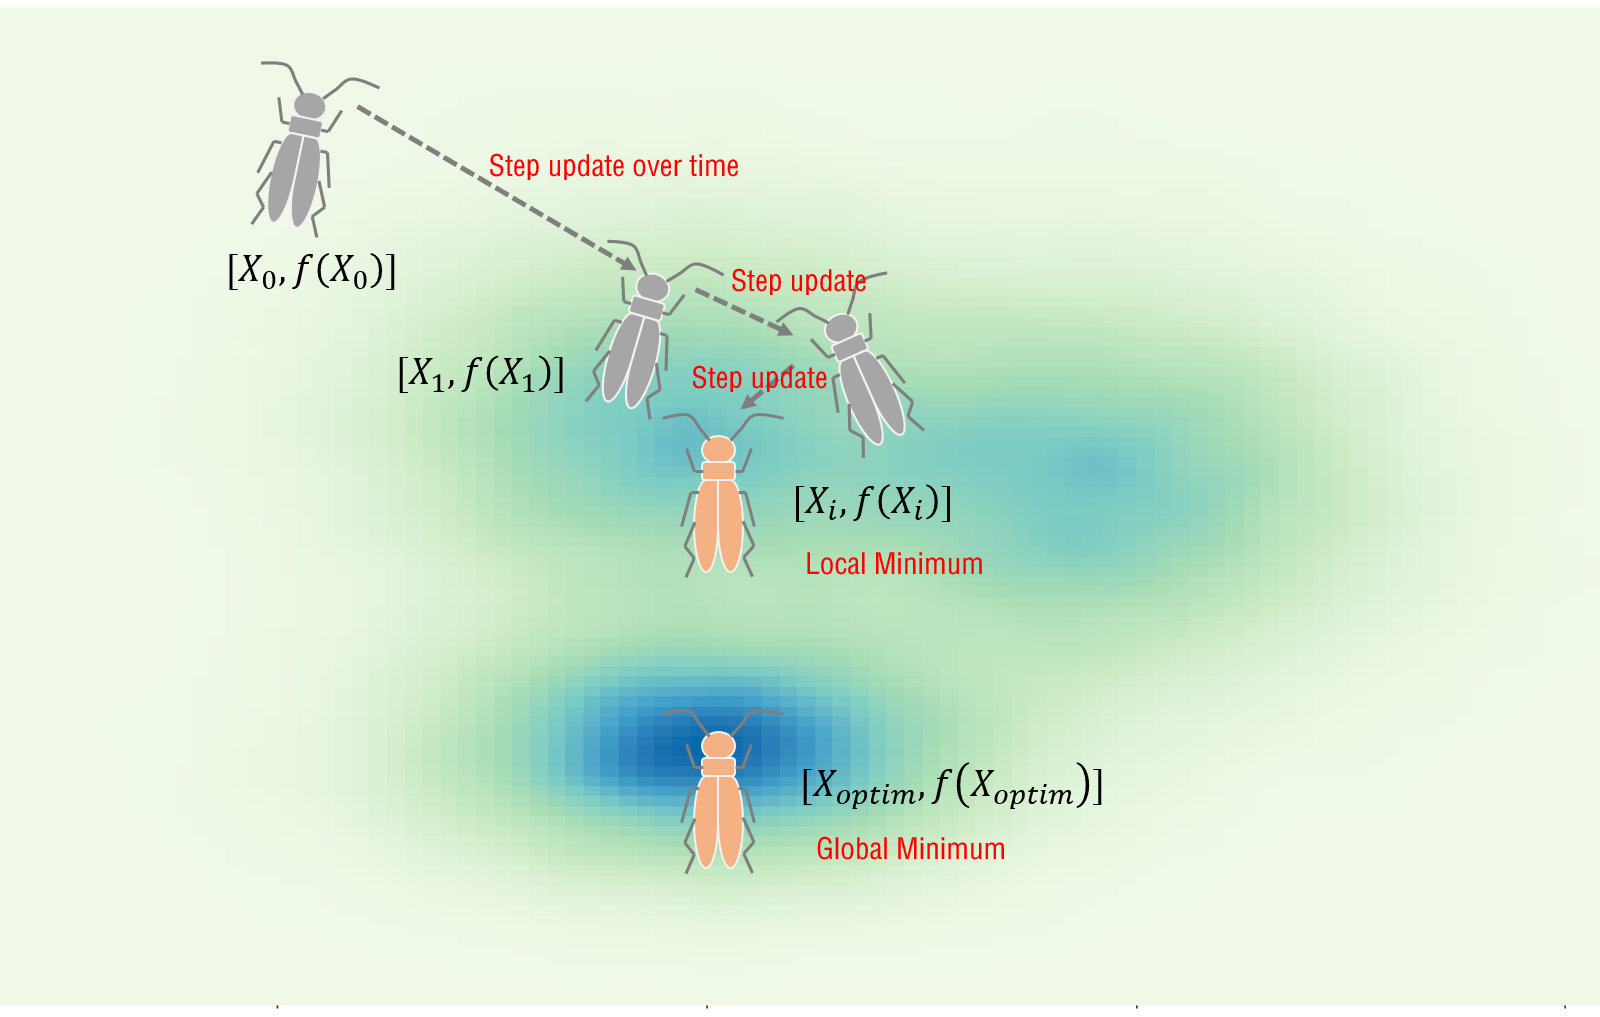
\includegraphics[width=0.8\linewidth]{img/BAS} 

}

\caption{BAS寻优过程示意}\label{fig:basflow}
\end{figure}

\begin{figure}

{\centering 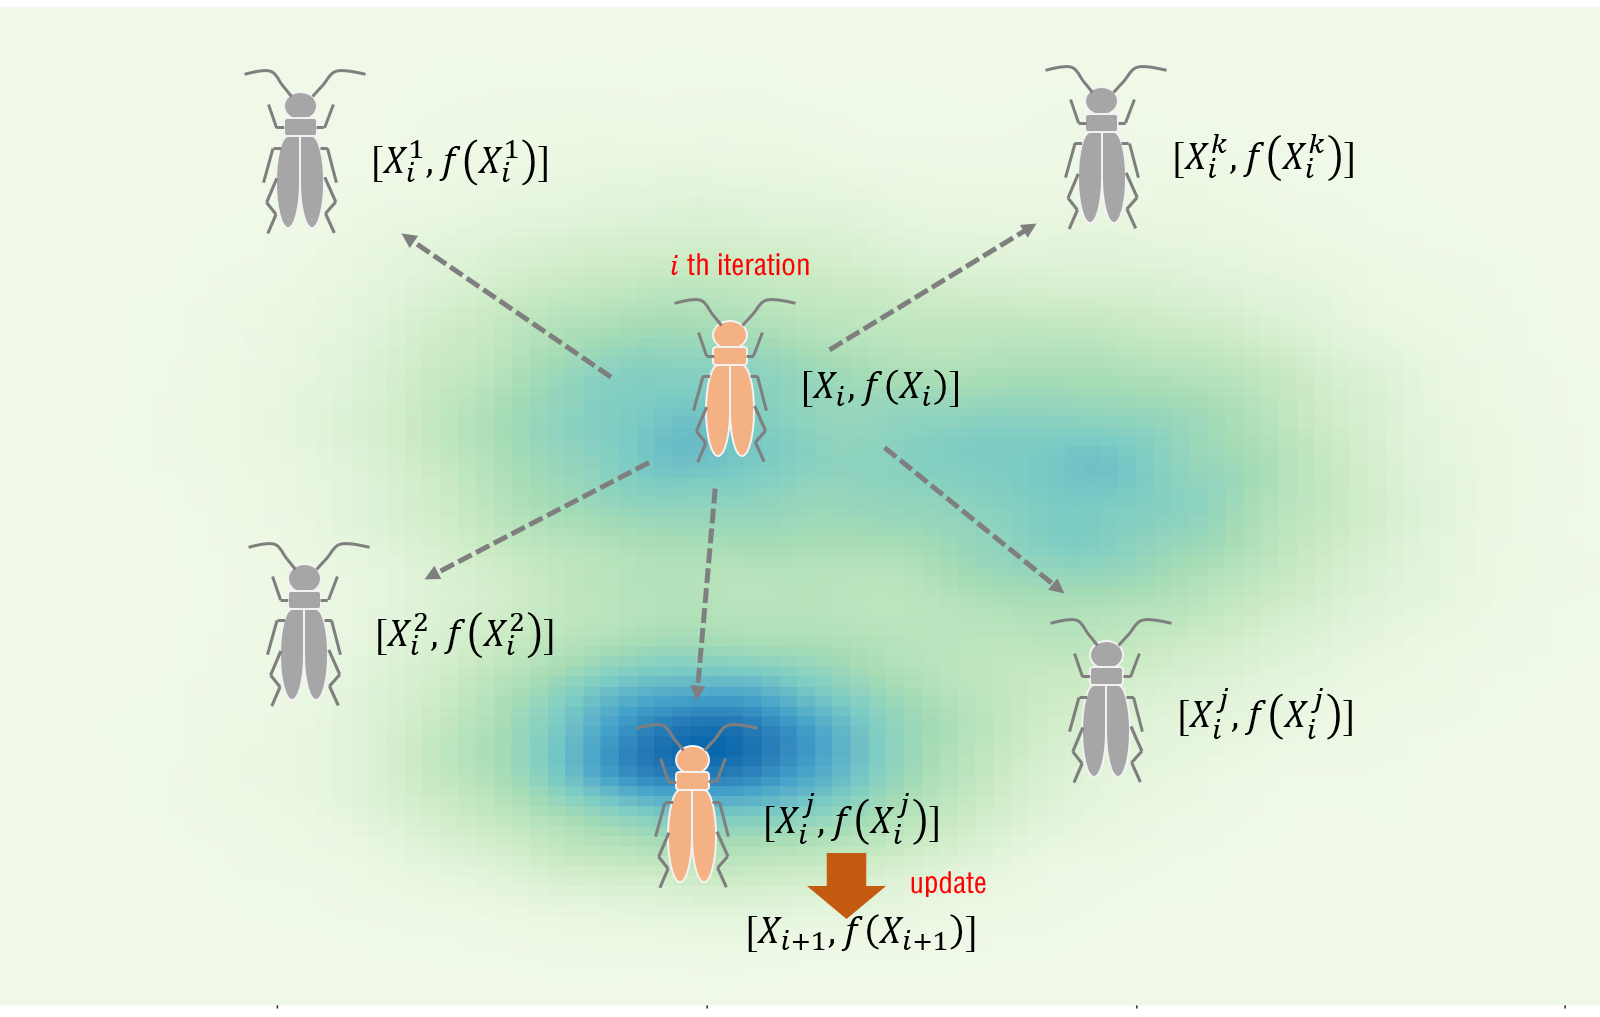
\includegraphics[width=0.8\linewidth]{img/BSAS} 

}

\caption{BSAS寻优过程示意}\label{fig:bsasflow}
\end{figure}

假定,天牛要找到图中\textbf{最蓝的点}。图\ref{fig:basflow}
中,天牛的起点在距离最优点较远处。由于位置更新只与时间有关,也就是每一步,天牛的步长都会缩减(为了可视化效果,天牛的大小我并没有缩放)。如果初始位置距离最优点较远,那在给定的步长缩减情况下,天牛只能在一个\textbf{局部最优点}处收敛。而图\ref{fig:bsasflow}中,每回合天牛会派出\(k\)只天牛在外试探,如果有更优的点,那么更新天牛位置。这样天牛可以更好地到达\textbf{全局最优点}。

\subsection{不足与改进}\label{BSASimprove}

虽然解决了步长更新和群体寻优的策略问题,但是还有两点并未解决。

\begin{itemize}
\tightlist
\item
  初始步长选取(参数标准化)

  \begin{itemize}
  \tightlist
  \item
    缺点:对于多参数且量纲相差较大的问题,步长 \(\delta\)
    的初始值并不好选取;
  \item
    改进:标准化参数后,再进行调节,这也是\texttt{BAS-WPT}的技巧所在;
  \end{itemize}
\item
  约束处理能力不足

  \begin{itemize}
  \tightlist
  \item
    缺点:在约束边界上优化目标突变问题的处理上表现不佳
  \item
    改进:二阶\texttt{BAS}
  \end{itemize}
\end{itemize}

好的是,在\texttt{rBAS\ 0.1.5}中,我们吸收了\texttt{BAS-WPT}中\textbf{参数标准化}的想法,加入了\texttt{BSAS-WPT}算法,来解决步长调参的问题,并取得了一定的改进效果。

\section{BAS-WPT}\label{bas-wpt}

相比于\ref{BASflow}节中描绘的\texttt{BAS},
\href{https://arxiv.org/abs/1711.02395}{Beetle Antennae Search without
Parameter Tuning (BAS-WPT) for Multi-objective
Optimization}一文给出了改进后的\texttt{BAS}是如何处理\textbf{步长调节}和\textbf{约束问题抽象}的。

\subsection{与BAS不同之处}\label{BASWPTflow}

\texttt{BAS-WPT}的小尾巴\texttt{without\ parameter\ tunning}已经说明了两者之间的区别,即\texttt{BAS-WPT}是不需要进行参数调节的。当然,按照我现在的理解,是\texttt{BAS-WPT}一方面简化了\textbf{每回合搜索距离}(质心到须的距离)的\textbf{更新},不需要再\textbf{额外设定与调节}诸如\(d_0\),\(\eta_d\)等参数,用户只需要按照式\eqref{eq:WPTupdate}来设置\(c_2\)便可;另一方面,参数标准化,让\textbf{存在量级差异}的参数之间不必再像\texttt{BAS}一样,共享一个你不知道该怎么设定的步长\(\delta^t\)(步长过大,小的参数可能经常处于在边界的状态;步长过小,大的参数可能搜索范围达不到)。

那么上述两方面的优势归纳起来是什么呢,那就是你可以设置一个在 \(1\) 附近
\(\delta\) ,然后设定一个衰减率
\(\eta_{\delta}\),以及步长与搜索距离之比
\(c_2\),那么你的天牛就不会出太大的岔子,并且方便调整调节。也就是说,\texttt{WPT}不是让你不用调参,而是减轻了调参的负担。

\begin{quote}
``不必就纠结归一化处理,之所以这么处理,仅仅是为了调参方便''

\begin{flushright}--- 姜向远\end{flushright}
\end{quote}

果然,偷懒催生了这一技巧的诞生。不过,我还得再次啰嗦一句标准化的好(是不是我没有接触这个领域,所以喜欢大惊小怪\ldots{}\ldots{})。我们在之后,压力容器约束问题(\textbf{混合整型规划})中,可以看到,待优化参数存在量级差异时,标准化技巧下的步长会比原始的\texttt{BAS}步长设定要更加合理。

\subsection{约束问题抽象形式}\label{constrform}

此外,\texttt{BAS-WPT}还为\texttt{BAS}引入了约束问题处理的手段。不过,这和我做模型预测控制时候看到的抽象方式是相同的。我觉得\texttt{BAS}的用户们应该都早已了解,此处就照本宣科。

\subsubsection{约束问题一般形式}

\begin{equation}
\begin{split}
& \frac{\text{Minimize}}{\text{Maximize}} f(\mathbf{x}) \\
s.t.  & g_j(\mathbf{x})\leq 0, j=1, \cdots, K \\
& x^\text{max}_i \leq x_i \leq x^\text{min}_i, i=1, \cdots N
\end{split}
\label{eq:ConProb}
\end{equation}

\(g_j(\mathbf{x})\leq 0\) 和
\(x^\text{max}_i \leq x_i \leq x^\text{min}_i\)
表示了参数本身的范围和更为精细具体的不等式约束控制。在\texttt{rBAS}包中,我们会有很\textbf{直观和简便}的方式,来设置这些约束。

\subsubsection{惩罚函数}

\begin{equation}
F(\mathbf{x})=f(\mathbf{x})+\lambda\sum_{j=1}^{K}h_j(\mathbf{x})g_j(\mathbf{x})
\label{eq:penalty}
\end{equation}

\begin{equation}
h_j(\mathbf{x}) = \begin{cases} 
1, & g_j(\mathbf{x})>0 \\ 
0, & g_j(\mathbf{x})\leq0
\end{cases}
\label{eq:violation}
\end{equation}

其中,式\eqref{eq:penalty}中的\(\lambda\)表示约束违背的惩罚因子,选取尽量大的正数。而后的\(h_j(\mathbf{x})\)为\texttt{Heaviside}函数,即不等式约束满足时,该函数为0,反之为1。

\subsection{不足与改进}\label{BSASimprove}

\begin{itemize}
\tightlist
\item
  约束处理能力不足

  \begin{itemize}
  \tightlist
  \item
    缺点:在约束边界上优化目标突变问题的处理上表现不佳
  \item
    改进:二阶\texttt{BAS}
  \end{itemize}
\end{itemize}

此处的不足,还需要考虑步长反馈和群体搜索的问题。不过,既然\texttt{BSAS}把姜博的\texttt{WPT}给窃来了,摇身变为了\texttt{BSAS-WPT},那就不说上述两个问题了。等他日有闲,再去整合\texttt{李晓晓}同学的二阶\texttt{BAS}。

\chapter{函数使用}\label{rBAS}

首先,加载\texttt{rBAS}包,然后在\ref{basoptim}节到\ref{bsaswpt}节中,我们详细讲述每个参数的含义。如果可能的话,我会加上调参时的经验(可能只对我的问题有用)。

\begin{Shaded}
\begin{Highlighting}[]
\KeywordTok{library}\NormalTok{(rBAS)}
\end{Highlighting}
\end{Shaded}

打开\href{https://jywang2016.github.io/rBAS/}{网址},可以看到托管在\texttt{github}上的\texttt{rBAS}文档。大家可以通过\texttt{Reference}来访问里面所有函数的帮助文档,通过\texttt{Changelog}来看每次包的更新及\texttt{bugs}修复记录。

\begin{quote}
文档网页是由\href{http://pkgdown.r-lib.org/}{\texttt{pkgdown}}包制作而成,logo由\href{https://github.com/GuangchuangYu/hexSticker}{\texttt{hexSticker}}包制作。
\end{quote}

\section{BASoptim}\label{basoptim}

除了通过访问函数文档网站外,还可以在\texttt{R}中输入下面的命令,来查看文档。

\begin{Shaded}
\begin{Highlighting}[]
\KeywordTok{help}\NormalTok{(BASoptim)}
\end{Highlighting}
\end{Shaded}

\subsection{BASoptim参数说明}\label{BASparms}

\href{https://jywang2016.github.io/rBAS/reference/BASoptim.html}{\texttt{BASoptim}函数}(对应\texttt{BAS}算法)调用的格式如下:

\begin{Shaded}
\begin{Highlighting}[]
\KeywordTok{BASoptim}\NormalTok{(fn, }
         \DataTypeTok{init =} \OtherTok{NULL}\NormalTok{, }
         \DataTypeTok{lower =} \KeywordTok{c}\NormalTok{(}\OperatorTok{-}\DecValTok{6}\NormalTok{, }\DecValTok{0}\NormalTok{), }\DataTypeTok{upper =} \KeywordTok{c}\NormalTok{(}\OperatorTok{-}\DecValTok{1}\NormalTok{, }\DecValTok{2}\NormalTok{),}
         \DataTypeTok{constr =} \OtherTok{NULL}\NormalTok{, }\DataTypeTok{pen =} \FloatTok{1e+05}\NormalTok{,}
         \DataTypeTok{d0 =} \FloatTok{0.001}\NormalTok{, }\DataTypeTok{d1 =} \DecValTok{3}\NormalTok{, }\DataTypeTok{eta_d =} \FloatTok{0.95}\NormalTok{, }
         \DataTypeTok{l0 =} \DecValTok{0}\NormalTok{,}\DataTypeTok{l1 =} \DecValTok{0}\NormalTok{, }\DataTypeTok{eta_l =} \FloatTok{0.95}\NormalTok{, }
         \DataTypeTok{step =} \FloatTok{0.8}\NormalTok{, }\DataTypeTok{eta_step =} \FloatTok{0.95}\NormalTok{, }
         \DataTypeTok{n =} \DecValTok{200}\NormalTok{,}\DataTypeTok{steptol =} \FloatTok{0.01}\NormalTok{, }
         \DataTypeTok{seed =} \OtherTok{NULL}\NormalTok{, }\DataTypeTok{trace =}\NormalTok{ T )}
\end{Highlighting}
\end{Shaded}

由于英文蹩脚,所以大家看起包自带的文档会比较吃力。因此,在此处给出中文说明。

\begin{itemize}
\tightlist
\item
  已知条件:目标函数与约束

  \begin{itemize}
  \tightlist
  \item
    fn 待优化的目标函数
  \item
    init
    参数初始值,默认为\texttt{NULL},即在上下限内随机选取,也可以自行指定
  \item
    constr 不等式约束
  \item
    lower/upper 上下限
  \item
    pen 惩罚因子\(\lambda\)
  \end{itemize}
\item
  \texttt{BAS}待调参数

  \begin{itemize}
  \tightlist
  \item
    d0
    参见式\eqref{eq:dupdate}中所述的搜索距离(也就是质心到须的距离)参数,一个比较小的值,默认为0.001
  \item
    d1 初始的搜索距离,默认为3
  \item
    eta\_d 搜索距离的衰减系数
  \item
    l0/l1/eta\_l 这一系列关于\(l\) 的参数,来源于\textbf{BAS}\index{BAS}
    \citep{Jiang2017BAS}论文中给出的\texttt{matlab}代码。其作用在于每回合位置更新时,产生一个\textbf{随机抖动}\(x = x - step * dir * sign(fn(left) - fn(right)) + l *random(npars)\)
  \item
    step/eta\_step 步长以及步长的衰减率
  \item
    steptol 停止更新的步长临界值
  \item
    n 回合数或者迭代次数
  \end{itemize}
\item
  其他

  \begin{itemize}
  \tightlist
  \item
    seed
    给定随机种子,用来固定寻优结果。不同的种子,对结果的影响\textbf{非常大}。
  \item
    trace 是否显示寻优过程信息
  \end{itemize}
\end{itemize}

\subsection{BASoptim简单案例}\label{BASexamples}

这里采用\textbf{BAS}\index{BAS}
\citep{Jiang2017BAS}一文中给出的测试函数,即\texttt{Michalewicz\ function}
与 \texttt{Goldstein-Price\ function}。

\subsubsection{Michalewicz function}\label{BASmich}

\[
f(x)=\sum_{i=1}^{d=2}sin(x_i)[sin(\frac{ix_i^2}{\pi})]^{20}
\]
图\ref{fig:mich}为\texttt{Michalewicz}函数在给定的约束范围的三维示意图。可以看到,最小值在\(x = -5,y = 1.5\)的附近。

\begin{figure}

{\centering \includegraphics[width=0.8\linewidth]{img/mich} 

}

\caption{ Michalewicz函数示意}\label{fig:mich}
\end{figure}

我们先在\texttt{R}的脚本中构建出函数:

\begin{Shaded}
\begin{Highlighting}[]
\CommentTok{# <- 可以视作 = 即用等于号在此处也是可以的 }
\NormalTok{mich <-}\StringTok{ }\ControlFlowTok{function}\NormalTok{(x)\{}
\NormalTok{  y1 <-}\StringTok{ }\OperatorTok{-}\KeywordTok{sin}\NormalTok{(x[}\DecValTok{1}\NormalTok{])}\OperatorTok{*}\NormalTok{(}\KeywordTok{sin}\NormalTok{((x[}\DecValTok{1}\NormalTok{]}\OperatorTok{^}\DecValTok{2}\NormalTok{)}\OperatorTok{/}\NormalTok{pi))}\OperatorTok{^}\DecValTok{20}
\NormalTok{  y2 <-}\StringTok{ }\OperatorTok{-}\KeywordTok{sin}\NormalTok{(x[}\DecValTok{2}\NormalTok{])}\OperatorTok{*}\NormalTok{(}\KeywordTok{sin}\NormalTok{((}\DecValTok{2}\OperatorTok{*}\NormalTok{x[}\DecValTok{2}\NormalTok{]}\OperatorTok{^}\DecValTok{2}\NormalTok{)}\OperatorTok{/}\NormalTok{pi))}\OperatorTok{^}\DecValTok{20}
  \KeywordTok{return}\NormalTok{(y1}\OperatorTok{+}\NormalTok{y2)}
\NormalTok{\}}
\end{Highlighting}
\end{Shaded}

然后利用\texttt{rBAS}包中的\texttt{BASoptim}函数求解:

\begin{Shaded}
\begin{Highlighting}[]
\CommentTok{# 把BASoptim的寻优结果赋值给test}
\NormalTok{test<-}
\StringTok{  }\KeywordTok{BASoptim}\NormalTok{(}\DataTypeTok{fn =}\NormalTok{ mich,}
           \DataTypeTok{lower =} \KeywordTok{c}\NormalTok{(}\OperatorTok{-}\DecValTok{6}\NormalTok{,}\DecValTok{0}\NormalTok{), }\DataTypeTok{upper =} \KeywordTok{c}\NormalTok{(}\OperatorTok{-}\DecValTok{1}\NormalTok{,}\DecValTok{2}\NormalTok{),}
           \DataTypeTok{seed =} \DecValTok{1}\NormalTok{, }\DataTypeTok{n =} \DecValTok{100}\NormalTok{,}\DataTypeTok{trace =} \OtherTok{FALSE}\NormalTok{)}

\NormalTok{test}\OperatorTok{$}\NormalTok{par}
\end{Highlighting}
\end{Shaded}

\begin{verbatim}
## [1] -4.964687  1.575415
\end{verbatim}

\begin{Shaded}
\begin{Highlighting}[]
\NormalTok{test}\OperatorTok{$}\NormalTok{value}
\end{Highlighting}
\end{Shaded}

\begin{verbatim}
## [1] -1.966817
\end{verbatim}

可以看到,\texttt{BAS}在100个回合内找到了全局的最小值。非\texttt{R}用户可能对上下限的声明有点陌生,\texttt{c(-6,0)}中\texttt{c()},其实是声明了一个向量,这也是\texttt{R}里面最基本的数据类型,和\texttt{matlab}里面的\texttt{{[}-6\ 0{]}}效果类似。整体看来,代码还是很简洁的。

\subsubsection{Goldstein-Price function}\label{BASgold}

\begin{equation}
\begin{split}
f({x})=& [1+(x_1+x_2+1)^2(19-14x_1+3x_1^2-14x_2\notag \\
& +6x_1x_2+3x_2^2)][30+(2x_1-3X_2)^2(18-32x_1\notag  \\
& +12x_1^2+48x_2-36x_1x_2+27x_2^2)]\notag
\end{split}
\end{equation}

图\ref{fig:gold}为\texttt{Goldstein-Price}函数在给定的约束范围的三维示意图。可以看到,最小值在\(x = -5,y = 1.5\)的附近。图\ref{fig:mich}与\ref{fig:gold}均使用\href{https://plot.ly/r/}{\texttt{plotly}}绘制。

\begin{figure}

{\centering \includegraphics[width=0.8\linewidth]{img/gold} 

}

\caption{ Michalewicz函数示意}\label{fig:gold}
\end{figure}

函数构造:

\begin{Shaded}
\begin{Highlighting}[]
\NormalTok{gold <-}\StringTok{ }\ControlFlowTok{function}\NormalTok{(x)\{}
\NormalTok{  x1 <-}\StringTok{ }\NormalTok{x[}\DecValTok{1}\NormalTok{]}
\NormalTok{  x2 <-}\StringTok{ }\NormalTok{x[}\DecValTok{2}\NormalTok{]}
\NormalTok{  y1 <-}\StringTok{ }\DecValTok{1} \OperatorTok{+}\StringTok{ }\NormalTok{(x1 }\OperatorTok{+}\StringTok{ }\NormalTok{x2 }\OperatorTok{+}\StringTok{ }\DecValTok{1}\NormalTok{)}\OperatorTok{^}\DecValTok{2}\OperatorTok{*}
\StringTok{    }\NormalTok{(}\DecValTok{19} \OperatorTok{-}\StringTok{ }\DecValTok{14}\OperatorTok{*}\NormalTok{x1}\OperatorTok{+}\DecValTok{3}\OperatorTok{*}\NormalTok{x1}\OperatorTok{^}\DecValTok{2} \OperatorTok{-}\StringTok{ }\DecValTok{14}\OperatorTok{*}\NormalTok{x2 }\OperatorTok{+}\StringTok{ }\DecValTok{6}\OperatorTok{*}\NormalTok{x1}\OperatorTok{*}\NormalTok{x2 }\OperatorTok{+}\StringTok{ }\DecValTok{3}\OperatorTok{*}\NormalTok{x2}\OperatorTok{^}\DecValTok{2}\NormalTok{)}
\NormalTok{  y2 <-}\StringTok{ }\DecValTok{30} \OperatorTok{+}\StringTok{ }\NormalTok{(}\DecValTok{2}\OperatorTok{*}\NormalTok{x1 }\OperatorTok{-}\DecValTok{3}\OperatorTok{*}\NormalTok{x2)}\OperatorTok{^}\DecValTok{2}\OperatorTok{*}
\StringTok{    }\NormalTok{(}\DecValTok{18} \OperatorTok{-}\StringTok{ }\DecValTok{32}\OperatorTok{*}\NormalTok{x1 }\OperatorTok{+}\StringTok{ }\DecValTok{12}\OperatorTok{*}\NormalTok{x1}\OperatorTok{^}\DecValTok{2}\OperatorTok{+}\DecValTok{48}\OperatorTok{*}\NormalTok{x2}\OperatorTok{-}\DecValTok{36}\OperatorTok{*}\NormalTok{x1}\OperatorTok{*}\NormalTok{x2 }\OperatorTok{+}\StringTok{ }\DecValTok{27}\OperatorTok{*}\NormalTok{x2}\OperatorTok{^}\DecValTok{2}\NormalTok{)}
  \KeywordTok{return}\NormalTok{(y1}\OperatorTok{*}\NormalTok{y2)}
\NormalTok{\}}
\end{Highlighting}
\end{Shaded}

其中,\texttt{x{[}1{]}}表示向量\texttt{x}的第一个元素。举例,\texttt{x\ =\ c(1,2)},那么\texttt{x{[}1{]}}等于1,\texttt{x{[}2{]}}等于2。索引从1开始,并不是从0开始(\texttt{python}和\texttt{C++}用户可能需要在此处注意)。

优化代码:

\begin{Shaded}
\begin{Highlighting}[]
\NormalTok{test<-}
\StringTok{  }\KeywordTok{BASoptim}\NormalTok{(}\DataTypeTok{fn =}\NormalTok{ gold,}
           \DataTypeTok{lower =} \KeywordTok{c}\NormalTok{(}\OperatorTok{-}\DecValTok{2}\NormalTok{,}\OperatorTok{-}\DecValTok{2}\NormalTok{), }\DataTypeTok{upper =} \KeywordTok{c}\NormalTok{(}\DecValTok{2}\NormalTok{,}\DecValTok{2}\NormalTok{),}
           \DataTypeTok{seed =} \OtherTok{NULL}\NormalTok{, }\DataTypeTok{n =} \DecValTok{100}\NormalTok{,}\DataTypeTok{trace =}\NormalTok{ F)}

\NormalTok{test}\OperatorTok{$}\NormalTok{par}
\end{Highlighting}
\end{Shaded}

\begin{verbatim}
## [1]  0.001870855 -0.996496153
\end{verbatim}

\begin{Shaded}
\begin{Highlighting}[]
\NormalTok{test}\OperatorTok{$}\NormalTok{value}
\end{Highlighting}
\end{Shaded}

\begin{verbatim}
## [1] 3.004756
\end{verbatim}

同样,结果也是给出了全局最优点(或在此附近,继续迭代下去,可能会有更精确更小的值)。

\section{BSASoptim}\label{bsasoptim}

\href{https://jywang2016.github.io/rBAS/reference/BSASoptim.html}{\texttt{BSASoptim}函数}(对应\texttt{BSAS}算法),在\texttt{BAS}的基础上,加入了步长反馈和群体策略。调用的格式如下:

\begin{Shaded}
\begin{Highlighting}[]
\KeywordTok{BSASoptim}\NormalTok{(fn, }
          \DataTypeTok{init =} \OtherTok{NULL}\NormalTok{, }\DataTypeTok{constr =} \OtherTok{NULL}\NormalTok{, }
          \DataTypeTok{lower =} \KeywordTok{c}\NormalTok{(}\OperatorTok{-}\DecValTok{6}\NormalTok{, }\DecValTok{0}\NormalTok{), }\DataTypeTok{upper =} \KeywordTok{c}\NormalTok{(}\OperatorTok{-}\DecValTok{1}\NormalTok{, }\DecValTok{2}\NormalTok{),}
          \DataTypeTok{k =} \DecValTok{5}\NormalTok{, }\DataTypeTok{pen =} \FloatTok{1e+05}\NormalTok{,}
          \DataTypeTok{d0 =} \FloatTok{0.001}\NormalTok{, }\DataTypeTok{d1 =} \DecValTok{3}\NormalTok{, }\DataTypeTok{eta_d =} \FloatTok{0.95}\NormalTok{,}
          \DataTypeTok{l0 =} \DecValTok{0}\NormalTok{, }\DataTypeTok{l1 =} \DecValTok{0}\NormalTok{, }\DataTypeTok{eta_l =} \FloatTok{0.95}\NormalTok{, }
          \DataTypeTok{step =} \FloatTok{0.8}\NormalTok{, }\DataTypeTok{eta_step =} \FloatTok{0.95}\NormalTok{,}\DataTypeTok{steptol =} \FloatTok{0.01}\NormalTok{,}
          \DataTypeTok{n =} \DecValTok{200}\NormalTok{, }\DataTypeTok{seed =} \OtherTok{NULL}\NormalTok{, }\DataTypeTok{trace =}\NormalTok{ T,  }
          \DataTypeTok{p_min =} \FloatTok{0.2}\NormalTok{,}\DataTypeTok{p_step =} \FloatTok{0.2}\NormalTok{, }\DataTypeTok{n_flag =} \DecValTok{2}\NormalTok{)}
\end{Highlighting}
\end{Shaded}

\subsection{BSASoptim参数说明}\label{BSASparms}

与\texttt{BAS}相比,\texttt{BSAS}在下面几处不同参数:

\begin{itemize}
\tightlist
\item
  k
  每回合的外出试探的天牛数目,越多结果会越稳定(多次执行,结果更接近),但是计算时长会相应增长。适当选取天牛数目,有助于避免随机的初始值和方向带来影响的同时,计算时长也可以接受。
\item
  p\_min
  当k只外出的天牛存在超过1只找到了更优的位置,也就是比当前的最佳值要更小。那是否需要\textbf{更新到那k只天牛中最优的那一只所在的位置呢}?经过一些尝试,我片面地认为,未必是每次都最佳,最后的位置一定最佳。因此,给定一个概率\(p_{min}\)。当有2只或以上的天牛找到更好的位置时,会在{[}0,1{]}间生成一个随机数,如果大于\(p_{min}\),那么就选k只天牛里\textbf{最优天牛}作为下次的更新位置牛;如果小于\(p_{min}\),那么就在找到了更好的位置的天牛里面,\textbf{随机选出}一只天牛,作为下次的更新位置。
\item
  p\_step
  想法与\texttt{p\_min}类同,用于\textbf{控制步长反馈策略}。在k只天牛找不到更优位置时,算法认为是步长过大,下一回合天牛位置不更新,且会减小步长。反之,则更新天牛位置,并保持当前步长直至不能找到更优位置。\textbf{那么,是否存在由于随机方向的原因,或者是k过小,导致在当前步长条件下,存在更优位置,但是找不到}。这个时候,我们设置一个更新概率\(p_{step}\),即在找不到更优的天牛位置下,步长有\(p_{step}\)概率不更新,继续寻找。
\item
  n\_flag
  为了防止设定过大的\texttt{p\_step},让数次产生的随机数都小于\texttt{p\_step},影响迭代的效率。我们给定了这个参数,默认为2,只要在同一个步长上的无效搜索(因为找不到更优位置而反复搜索)次数保持3次及以上,则会强制更新步长。
\end{itemize}

\subsection{BSASoptim取值摸索}\label{BSAStrick}

好吧,用中文说明都这么绕口,何况是我撰写的可怜的英文文档。有同学会问了,为什么要后面那几个概率和什么次数的参数,这不是画蛇添足吗?回答是,这几个参数\textbf{来源于生活}···

我在做建筑阻容模型系统辨识时,每回合的寻优,都是在用龙哥库塔法求解一次常微分方程组(\texttt{ODEs})。在我的问题规模下,每回合纯粹的R代码要\textbf{耗费0.25s左右}来求解一次这样的\texttt{ODEs}。也就是说,在求解目标函数上,程序耗费的时间就有\(k*n*0.25\),还不算其他的计算开销。(换言之,用遗传算法,会带来更大的计算开销,因为每回合至少计算10*参数个数次的目标函数)

所以,我必须要结果较好的同时,尽量减少不必要的计算。因此,k不能太大,但是这又会在随机方向的影响下,\textbf{错失一些优化的位置},那就需要\texttt{p\_step}参数了。但是初始位置或者说中间位置附近的最优,\textbf{不代表在这附近或方向上,有全局最优},所以我还需要\texttt{p\_min}来保证,我有那么\textbf{一丝可能},跳出\textbf{每次都找最优,可是收敛结果与全局最优背离}的怪圈。至于\texttt{n\_flag},是因为我之前设置了\texttt{p\_step}为0.5,所以算法效率极低,几乎每个找不到更优的夜,这些天牛都悲伤地多做数次运行,所以我设置了这个参数。

\begin{quote}
还是需要强调,在我的问题里,这些参数起到了较好的效果。但是换成大家的研究,这些参数可能就是被害妄想症的产物了。有意思的是,我在默认参数下执行50次
\texttt{Michalewicz}
函数的寻优,效果并没有\texttt{BASoptim}好。但在RC模型辨识上,\texttt{BSASoptim}远好于\texttt{BASoptim}。
\end{quote}

接下来就是这几个参数的调节的一些小技巧了。

\begin{itemize}
\tightlist
\item
  设置\texttt{k}为1,那就是带步长反馈的BAS了
\item
  如果求解目标函数速度快,可以设置较大的k
\item
  \texttt{p\_step}设置为0,只要k只天牛找不到最优位置,步长就会更新;不存在不更新继续找的可能
\item
  \texttt{p\_step}设置为1,那算法会在一个步长下一直执行,直到找到更优的位置,才会更新步长
\item
  \texttt{p\_min}设置为0,在k只出去试探的天牛中找到了更优的位置时,那么当前时刻的天牛,总会选择这k只中最好的一只的位置来作为下一时刻的位置
\item
  \texttt{p\_min}设置为1,下一时刻的位置是k只中更优天牛的位置的随机选择
\item
  为了求解效率,\texttt{p\_step}会选择较小的值;\texttt{p\_min}我也没有摸清楚个规律,但是在我的研究对象中,为0得到的结果在多次试验中,整体看来没有为较小值0.2好。
\end{itemize}

上述是我在自身研究方向上摸出的规律,可能问题的类型不同,需要做的取舍也不同。大家可以保持默认参数,然后进行符合自身情况的微调。更为详细的结果可以参见\textbf{BSAS}\index{BSAS}
\citep{Wang2018BSAS}论文。

\subsection{BSASoptim案例}\label{BSASexample}

\subsubsection{Michalewicz function}\label{michalewicz-function}

不做过多的阐述对于此案例,可以参看\ref{BASmich}节。

\begin{Shaded}
\begin{Highlighting}[]
\KeywordTok{library}\NormalTok{(rBAS)}
\NormalTok{mich <-}\StringTok{ }\ControlFlowTok{function}\NormalTok{(x)\{}
\NormalTok{   y1 <-}\StringTok{ }\OperatorTok{-}\KeywordTok{sin}\NormalTok{(x[}\DecValTok{1}\NormalTok{])}\OperatorTok{*}\NormalTok{(}\KeywordTok{sin}\NormalTok{((x[}\DecValTok{1}\NormalTok{]}\OperatorTok{^}\DecValTok{2}\NormalTok{)}\OperatorTok{/}\NormalTok{pi))}\OperatorTok{^}\DecValTok{20}
\NormalTok{   y2 <-}\StringTok{ }\OperatorTok{-}\KeywordTok{sin}\NormalTok{(x[}\DecValTok{2}\NormalTok{])}\OperatorTok{*}\NormalTok{(}\KeywordTok{sin}\NormalTok{((}\DecValTok{2}\OperatorTok{*}\NormalTok{x[}\DecValTok{2}\NormalTok{]}\OperatorTok{^}\DecValTok{2}\NormalTok{)}\OperatorTok{/}\NormalTok{pi))}\OperatorTok{^}\DecValTok{20}
   \KeywordTok{return}\NormalTok{(y1}\OperatorTok{+}\NormalTok{y2)}
\NormalTok{\}}
\NormalTok{result <-}\StringTok{ }\KeywordTok{BSASoptim}\NormalTok{(}\DataTypeTok{fn =}\NormalTok{ mich,}
                    \DataTypeTok{lower =} \KeywordTok{c}\NormalTok{(}\OperatorTok{-}\DecValTok{6}\NormalTok{,}\DecValTok{0}\NormalTok{), }\DataTypeTok{upper =} \KeywordTok{c}\NormalTok{(}\OperatorTok{-}\DecValTok{1}\NormalTok{,}\DecValTok{2}\NormalTok{),}
                    \DataTypeTok{seed =} \DecValTok{1}\NormalTok{, }\DataTypeTok{n =} \DecValTok{100}\NormalTok{,}\DataTypeTok{k=}\DecValTok{5}\NormalTok{,}\DataTypeTok{step =} \FloatTok{0.6}\NormalTok{,}
                    \DataTypeTok{trace =} \OtherTok{FALSE}\NormalTok{)}
\NormalTok{result}\OperatorTok{$}\NormalTok{par}
\end{Highlighting}
\end{Shaded}

\begin{verbatim}
## [1] -4.970202  1.578791
\end{verbatim}

\begin{Shaded}
\begin{Highlighting}[]
\NormalTok{result}\OperatorTok{$}\NormalTok{value}
\end{Highlighting}
\end{Shaded}

\begin{verbatim}
## [1] -1.963534
\end{verbatim}

\subsubsection{Pressure Vessel function}\label{BSASpv}

使用\textbf{BAS-WPT}\index{BAS-WPT}\citep{Jiangwpt}
论文中压力容器优化函数来测试\texttt{BSASoptim}处理约束的能力。问题背景如下:

\begin{align}
\text{minimize} f(\mathbf{x}) = &0.6224x_1x_3x_4+1.7781x_2x^2_3 \notag\\
&+3.1661x^2_1x_4 + 19.84x^2_1x_3 \notag \\
s.t. ~~ g_1(\mathbf{x}) = & -x1 + 0.0193x_3 \leq 0 \notag \\
g_2(\mathbf{x}) = & -x_2 + 0.00954x_3 \leq 0 \notag \\
g_3(\mathbf{x}) = & -\pi x^2_3x_4 -\frac{4}{3}\pi x^3_3 + 1296000 \leq 0 \notag \\
g_4(\mathbf{x}) = & x_4-240\leq 0 \notag \\
x_1 \in& \{1,2,3,\cdots,99\}\times0.0625 \notag \\
x_2 \in& \{1,2,3,\cdots,99\}\times0.0625 \notag \\
x_3 \in& [10,200] \notag \\
x_4 \in& [10,200] \notag \\
\label{eq:PV}
\end{align}

构造一个列表,也就是\texttt{list()}。其中包含有2个函数,一个是我们的目标函数\texttt{obj},一个是我们的不等式约束函数\texttt{con}。为了方便起见,我并没有写每一个函数的返回值,那么,\texttt{R}会自动返回计算的最后一个对象。比如,在\texttt{obj}函数中,是\texttt{result}变量(标量)被返回。而在\texttt{con}函数中,是由\texttt{c()}声明的向量被返回。

\begin{Shaded}
\begin{Highlighting}[]
\NormalTok{pressure_Vessel <-}\StringTok{ }\KeywordTok{list}\NormalTok{(}
  \DataTypeTok{obj =} \ControlFlowTok{function}\NormalTok{(x)\{}
\NormalTok{    x1 <-}\StringTok{ }\KeywordTok{floor}\NormalTok{(x[}\DecValTok{1}\NormalTok{])}\OperatorTok{*}\FloatTok{0.0625}
\NormalTok{    x2 <-}\StringTok{ }\KeywordTok{floor}\NormalTok{(x[}\DecValTok{2}\NormalTok{])}\OperatorTok{*}\FloatTok{0.0625}
\NormalTok{    x3 <-}\StringTok{ }\NormalTok{x[}\DecValTok{3}\NormalTok{]}
\NormalTok{    x4 <-}\StringTok{ }\NormalTok{x[}\DecValTok{4}\NormalTok{]}
\NormalTok{    result <-}\StringTok{ }\FloatTok{0.6224}\OperatorTok{*}\NormalTok{x1}\OperatorTok{*}\NormalTok{x3}\OperatorTok{*}\NormalTok{x4 }\OperatorTok{+}\StringTok{ }
\StringTok{      }\FloatTok{1.7781}\OperatorTok{*}\NormalTok{x2}\OperatorTok{*}\NormalTok{x3}\OperatorTok{^}\DecValTok{2} \OperatorTok{+}
\StringTok{      }\FloatTok{3.1611}\OperatorTok{*}\NormalTok{x1}\OperatorTok{^}\DecValTok{2}\OperatorTok{*}\NormalTok{x4 }\OperatorTok{+}\StringTok{ }
\StringTok{      }\FloatTok{19.84}\OperatorTok{*}\NormalTok{x1}\OperatorTok{^}\DecValTok{2}\OperatorTok{*}\NormalTok{x3}
\NormalTok{  \},}
  \DataTypeTok{con =} \ControlFlowTok{function}\NormalTok{(x)\{}
\NormalTok{    x1 <-}\StringTok{ }\KeywordTok{floor}\NormalTok{(x[}\DecValTok{1}\NormalTok{])}\OperatorTok{*}\FloatTok{0.0625}
\NormalTok{    x2 <-}\StringTok{ }\KeywordTok{floor}\NormalTok{(x[}\DecValTok{2}\NormalTok{])}\OperatorTok{*}\FloatTok{0.0625}
\NormalTok{    x3 <-}\StringTok{ }\NormalTok{x[}\DecValTok{3}\NormalTok{]}
\NormalTok{    x4 <-}\StringTok{ }\NormalTok{x[}\DecValTok{4}\NormalTok{]}
    \KeywordTok{c}\NormalTok{(}\CommentTok{#把所有的不等式约束,全部写为小于等于0的形式}
      \FloatTok{0.0193}\OperatorTok{*}\NormalTok{x3 }\OperatorTok{-}\StringTok{ }\NormalTok{x1,}
      \FloatTok{0.00954}\OperatorTok{*}\NormalTok{x3 }\OperatorTok{-}\StringTok{ }\NormalTok{x2,}
      \FloatTok{750.0}\OperatorTok{*}\FloatTok{1728.0} \OperatorTok{-}\StringTok{ }\NormalTok{pi}\OperatorTok{*}\NormalTok{x3}\OperatorTok{^}\DecValTok{2}\OperatorTok{*}\NormalTok{x4 }\OperatorTok{-}\StringTok{ }\DecValTok{4}\OperatorTok{/}\DecValTok{3}\OperatorTok{*}\NormalTok{pi}\OperatorTok{*}\NormalTok{x3}\OperatorTok{^}\DecValTok{3}
\NormalTok{    )}
\NormalTok{  \}}
\NormalTok{)}
\end{Highlighting}
\end{Shaded}

使用\texttt{BSASoptim}函数进行优化。需要注意的是,\texttt{pressure\_Vessel}是一个列表,对于其中包含的元素,使用\texttt{\$}符号进行访问。也可以使用\texttt{{[}{[}}符号,即
\texttt{pressure\_Vessel\$obj} 等价于
\texttt{pressure\_Vessel{[}{[}1{]}{]}}。

\begin{Shaded}
\begin{Highlighting}[]
\NormalTok{result <-}\StringTok{ }\KeywordTok{BSASoptim}\NormalTok{(}\DataTypeTok{fn =}\NormalTok{ pressure_Vessel}\OperatorTok{$}\NormalTok{obj,}
                    \DataTypeTok{k =} \DecValTok{5}\NormalTok{,}
                    \DataTypeTok{lower =}\KeywordTok{c}\NormalTok{( }\DecValTok{1}\NormalTok{, }\DecValTok{1}\NormalTok{, }\DecValTok{10}\NormalTok{, }\DecValTok{10}\NormalTok{),}
                    \DataTypeTok{upper =} \KeywordTok{c}\NormalTok{(}\DecValTok{100}\NormalTok{, }\DecValTok{100}\NormalTok{, }\DecValTok{200}\NormalTok{, }\DecValTok{200}\NormalTok{),}
                    \DataTypeTok{constr =}\NormalTok{ pressure_Vessel}\OperatorTok{$}\NormalTok{con,}
                    \DataTypeTok{n =} \DecValTok{200}\NormalTok{,}
                    \DataTypeTok{step =} \DecValTok{100}\NormalTok{,}
                    \DataTypeTok{d1 =} \DecValTok{5}\NormalTok{,}
                    \DataTypeTok{pen =} \FloatTok{1e6}\NormalTok{,}
                    \DataTypeTok{steptol =} \FloatTok{1e-6}\NormalTok{,}
                    \DataTypeTok{n_flag =} \DecValTok{2}\NormalTok{,}
                    \DataTypeTok{seed =} \DecValTok{2}\NormalTok{,}\DataTypeTok{trace =} \OtherTok{FALSE}\NormalTok{)}

\NormalTok{result}\OperatorTok{$}\NormalTok{par}
\end{Highlighting}
\end{Shaded}

\begin{verbatim}
## [1]  14.92195   7.87620  43.51377 159.87104
\end{verbatim}

\begin{Shaded}
\begin{Highlighting}[]
\NormalTok{result}\OperatorTok{$}\NormalTok{value}
\end{Highlighting}
\end{Shaded}

\begin{verbatim}
## [1] 6309.406
\end{verbatim}

可以看到结果与论文\textbf{BAS-WPT}\index{BAS-WPT}\citep{Jiangwpt}中\texttt{TABLE\ 1}给出的优化值还是有一定的差距。不过,这也让我意识到了,对于\textbf{复杂的优化问题,调试其中的参数是个困难的活}。歧路亡羊呀!

好在,改进后的\texttt{BSAS-WPT}能够比较好地得到不逊于\textbf{BAS-WPT}\index{BAS-WPT}\citep{Jiangwpt}中的结果(在\ref{bsaswptexample}节可以看到)。更多更优地结果,等待你去调参,如果你还有勇气的话。

\subsubsection{Himmelblau function}\label{BSAShim}

\begin{align}
\text{minimize} f(\mathbf{x}) =& 5.3578547x^2_3 +0.8356891x_1x_5\notag \\
&+ 37.29329x_1 - 40792.141 \notag\\
s.t. ~~g_1(\mathbf{x}) =& 85.334407 + 0.0056858x_2x_5\notag\\
&+ 0.00026x_1x_4 - 0.0022053x_3x_5  \notag\\
g_2(\mathbf{x}) =&80.51249 +0.0071317x_2x_5\notag\\
&+ 0.0029955x_1x_2 + 0.0021813x^2_3  \notag\\
g_3(\mathbf{x}) =& 9.300961 +0.0047026x_3x_5\notag\\
&+ 0.0012547x_1x_3 + 0.0019085x_3x_4 \notag\\
g_1(\mathbf{x})\in&[0,92] \notag\\
g_2(\mathbf{x})\in&[90,110] \notag\\
g_3(\mathbf{x})\in&[20,25] \notag\\
x_1\in&[78,102] \notag\\
x_2\in&[33,45] \notag\\
x_3\in&[27,45] \notag\\
x_4\in&[27,45] \notag\\
x_5\in&[27,45] \notag\\
\label{eq:him}
\end{align}

构造优化目标函数和约束:

\begin{Shaded}
\begin{Highlighting}[]
\NormalTok{himmelblau <-}\StringTok{ }\KeywordTok{list}\NormalTok{(}
  \DataTypeTok{obj =} \ControlFlowTok{function}\NormalTok{(x)\{}
\NormalTok{    x1 <-}\StringTok{ }\NormalTok{x[}\DecValTok{1}\NormalTok{]}
\NormalTok{    x3 <-}\StringTok{ }\NormalTok{x[}\DecValTok{3}\NormalTok{]}
\NormalTok{    x5 <-}\StringTok{ }\NormalTok{x[}\DecValTok{5}\NormalTok{]}
\NormalTok{    result <-}\StringTok{ }\FloatTok{5.3578547}\OperatorTok{*}\NormalTok{x3}\OperatorTok{^}\DecValTok{2} \OperatorTok{+}\StringTok{ }
\StringTok{      }\FloatTok{0.8356891}\OperatorTok{*}\NormalTok{x1}\OperatorTok{*}\NormalTok{x5 }\OperatorTok{+}\StringTok{ }
\StringTok{      }\FloatTok{37.29329}\OperatorTok{*}\NormalTok{x[}\DecValTok{1}\NormalTok{] }\OperatorTok{-}\StringTok{ }
\StringTok{      }\FloatTok{40792.141}
\NormalTok{  \},}
  \DataTypeTok{con =} \ControlFlowTok{function}\NormalTok{(x)\{}
\NormalTok{    x1 <-}\StringTok{ }\NormalTok{x[}\DecValTok{1}\NormalTok{]}
\NormalTok{    x2 <-}\StringTok{ }\NormalTok{x[}\DecValTok{2}\NormalTok{]}
\NormalTok{    x3 <-}\StringTok{ }\NormalTok{x[}\DecValTok{3}\NormalTok{]}
\NormalTok{    x4 <-}\StringTok{ }\NormalTok{x[}\DecValTok{4}\NormalTok{]}
\NormalTok{    x5 <-}\StringTok{ }\NormalTok{x[}\DecValTok{5}\NormalTok{]}
\NormalTok{    g1 <-}\StringTok{ }\FloatTok{85.334407} \OperatorTok{+}\StringTok{ }\FloatTok{0.0056858}\OperatorTok{*}\NormalTok{x2}\OperatorTok{*}\NormalTok{x5 }\OperatorTok{+}\StringTok{ }
\StringTok{      }\FloatTok{0.00026}\OperatorTok{*}\NormalTok{x1}\OperatorTok{*}\NormalTok{x4 }\OperatorTok{-}\StringTok{ }\FloatTok{0.0022053}\OperatorTok{*}\NormalTok{x3}\OperatorTok{*}\NormalTok{x5}
\NormalTok{    g2 <-}\StringTok{ }\FloatTok{80.51249} \OperatorTok{+}\StringTok{ }\FloatTok{0.0071317}\OperatorTok{*}\NormalTok{x2}\OperatorTok{*}\NormalTok{x5 }\OperatorTok{+}\StringTok{ }
\StringTok{      }\FloatTok{0.0029955}\OperatorTok{*}\NormalTok{x1}\OperatorTok{*}\NormalTok{x2 }\OperatorTok{+}\StringTok{ }\FloatTok{0.0021813}\OperatorTok{*}\NormalTok{x3}\OperatorTok{^}\DecValTok{2}
\NormalTok{    g3 <-}\StringTok{ }\FloatTok{9.300961} \OperatorTok{+}\StringTok{ }\FloatTok{0.0047026}\OperatorTok{*}\NormalTok{x3}\OperatorTok{*}\NormalTok{x5 }\OperatorTok{+}\StringTok{ }
\StringTok{      }\FloatTok{0.0012547}\OperatorTok{*}\NormalTok{x1}\OperatorTok{*}\NormalTok{x3 }\OperatorTok{+}\StringTok{ }\FloatTok{0.0019085}\OperatorTok{*}\NormalTok{x3}\OperatorTok{*}\NormalTok{x4}
    \KeywordTok{c}\NormalTok{(}
      \OperatorTok{-}\NormalTok{g1,}
\NormalTok{      g1}\OperatorTok{-}\DecValTok{92}\NormalTok{,}
      \DecValTok{90}\OperatorTok{-}\NormalTok{g2,}
\NormalTok{      g2 }\OperatorTok{-}\StringTok{ }\DecValTok{110}\NormalTok{,}
      \DecValTok{20} \OperatorTok{-}\StringTok{ }\NormalTok{g3,}
\NormalTok{      g3 }\OperatorTok{-}\StringTok{ }\DecValTok{25}
\NormalTok{    )}
\NormalTok{  \}}
\NormalTok{)}
\end{Highlighting}
\end{Shaded}

使用\texttt{BSASoptim}函数进行优化:

\begin{Shaded}
\begin{Highlighting}[]
\NormalTok{result <-}\StringTok{ }\KeywordTok{BSASoptim}\NormalTok{(}\DataTypeTok{fn =}\NormalTok{ himmelblau}\OperatorTok{$}\NormalTok{obj,}
                    \DataTypeTok{k =} \DecValTok{5}\NormalTok{,}
                    \DataTypeTok{lower =}\KeywordTok{c}\NormalTok{(}\DecValTok{78}\NormalTok{,}\DecValTok{33}\NormalTok{,}\DecValTok{27}\NormalTok{,}\DecValTok{27}\NormalTok{,}\DecValTok{27}\NormalTok{),}
                    \DataTypeTok{upper =} \KeywordTok{c}\NormalTok{(}\DecValTok{102}\NormalTok{,}\DecValTok{45}\NormalTok{,}\DecValTok{45}\NormalTok{,}\DecValTok{45}\NormalTok{,}\DecValTok{45}\NormalTok{),}
                    \DataTypeTok{constr =}\NormalTok{ himmelblau}\OperatorTok{$}\NormalTok{con,}
                    \DataTypeTok{n =} \DecValTok{200}\NormalTok{,}
                    \DataTypeTok{step =} \DecValTok{100}\NormalTok{,}
                    \DataTypeTok{d1 =} \DecValTok{10}\NormalTok{,}
                    \DataTypeTok{pen =} \FloatTok{1e6}\NormalTok{,}
                    \DataTypeTok{steptol =} \FloatTok{1e-6}\NormalTok{,}
                    \DataTypeTok{n_flag =} \DecValTok{2}\NormalTok{,}
                    \DataTypeTok{seed =} \DecValTok{11}\NormalTok{,}\DataTypeTok{trace =} \OtherTok{FALSE}\NormalTok{)}
\NormalTok{result}\OperatorTok{$}\NormalTok{par }
\end{Highlighting}
\end{Shaded}

\begin{verbatim}
## [1] 78.01565 33.00000 27.07409 45.00000 44.95878
\end{verbatim}

\begin{Shaded}
\begin{Highlighting}[]
\NormalTok{result}\OperatorTok{$}\NormalTok{value}
\end{Highlighting}
\end{Shaded}

\begin{verbatim}
## [1] -31024.17
\end{verbatim}

这个结果,比\textbf{BAS-WPT}\index{BAS-WPT}\citep{Jiangwpt}中\texttt{TABLE\ 2}记载的结果都要好。但只要你愿意调差,嘿嘿,总有更好的。

\section{BSAS-WPT}\label{bsaswpt}

在进行\texttt{BSAS-WPT}参数讲解的这一部分前,我想问个问题。在式\eqref{eq:PV}和式\eqref{eq:him}中,我们可以看到,有些\(x_i\)的约束范围较小,有的较大。比如,压力容器中,\(x_1\)和\(x_2\)就偏小,只是经过提取出0.0625,勉强能达到\(x_3\)和\(x_4\)的一半。那么,如果某些优化问题,其参数约束范围之间,相差了量级,该\textbf{如何选择步长}呢?这就是\texttt{WPT}的便捷之处了。

\href{https://jywang2016.github.io/rBAS/reference/BSAS_WPT.html}{\texttt{BSAS-WPT}函数}(对应\texttt{BSAS-WPT}算法)调用的格式如下:

\begin{Shaded}
\begin{Highlighting}[]
\KeywordTok{BSAS_WPT}\NormalTok{(fn, }
         \DataTypeTok{init =} \OtherTok{NULL}\NormalTok{, }
         \DataTypeTok{lower =} \KeywordTok{c}\NormalTok{(}\OperatorTok{-}\DecValTok{6}\NormalTok{, }\DecValTok{0}\NormalTok{), }\DataTypeTok{upper =} \KeywordTok{c}\NormalTok{(}\OperatorTok{-}\DecValTok{1}\NormalTok{, }\DecValTok{2}\NormalTok{),}
         \DataTypeTok{k =} \DecValTok{5}\NormalTok{, }\DataTypeTok{constr =} \OtherTok{NULL}\NormalTok{, }\DataTypeTok{pen =} \FloatTok{1e+05}\NormalTok{, }
         \DataTypeTok{c2 =} \DecValTok{5}\NormalTok{, }
         \DataTypeTok{step =} \DecValTok{1}\NormalTok{, }\DataTypeTok{eta_step =} \FloatTok{0.95}\NormalTok{,}\DataTypeTok{steptol =} \FloatTok{0.001}\NormalTok{, }
         \DataTypeTok{n =} \DecValTok{200}\NormalTok{, }\DataTypeTok{seed =} \OtherTok{NULL}\NormalTok{, }\DataTypeTok{trace =}\NormalTok{ T, }
         \DataTypeTok{p_min =} \FloatTok{0.2}\NormalTok{,}\DataTypeTok{p_step =} \FloatTok{0.2}\NormalTok{, }\DataTypeTok{n_flag =} \DecValTok{2}\NormalTok{)}
\end{Highlighting}
\end{Shaded}

\subsection{BSAS-WPT 参数说明}\label{bsaswptparms}

与\texttt{BSAS}相比,除去我人为略去的抖动部分,减少了搜索距离\texttt{d}相关的参数,这些用\texttt{c2}来替代。而初始步长\texttt{step},我们可以设定为一个在1附近的数。由于算法先标准化了参数,然后根据式\eqref{eq:xupdate}在计算位置后,再根据上下限进行反标准化,而后导入目标函数。所以,你可以认为,\texttt{BSAS}中,把step变成一个\(n\)维的向量,假设\(n\)是参数个数,每个步长元素都根据参数的约束范围大小来设定,那么算法就会变成\texttt{BSAS-WPT}。

总之,现在要调节的参数,主要有2个,即\texttt{c2}和\texttt{step}。

\subsection{BSAS-WPT 案例}\label{bsaswptexample}

我们使用和\texttt{BSASoptim}函数相同的例子来对比效果。但是,这些效果都是不固定的,即给定不同的参数,结果也会不同,所以不能根据一次结果评价算法的优劣。

\subsubsection{Pressure Vessel function}\label{bsaswptPV}

\begin{Shaded}
\begin{Highlighting}[]
\NormalTok{result <-}\StringTok{ }\KeywordTok{BSAS_WPT}\NormalTok{(}\DataTypeTok{fn =}\NormalTok{ pressure_Vessel}\OperatorTok{$}\NormalTok{obj,}
                   \DataTypeTok{k =} \DecValTok{8}\NormalTok{,}
                   \DataTypeTok{lower =}\KeywordTok{c}\NormalTok{( }\DecValTok{1}\NormalTok{, }\DecValTok{1}\NormalTok{, }\DecValTok{10}\NormalTok{, }\DecValTok{10}\NormalTok{),}
                   \DataTypeTok{upper =} \KeywordTok{c}\NormalTok{(}\DecValTok{100}\NormalTok{, }\DecValTok{100}\NormalTok{, }\DecValTok{200}\NormalTok{, }\DecValTok{200}\NormalTok{),}
                   \DataTypeTok{constr =}\NormalTok{ pressure_Vessel}\OperatorTok{$}\NormalTok{con,}
                   \DataTypeTok{c2 =} \DecValTok{10}\NormalTok{, }\DataTypeTok{n =} \DecValTok{200}\NormalTok{, }\DataTypeTok{step =} \DecValTok{2}\NormalTok{,}
                   \DataTypeTok{seed =} \DecValTok{1}\NormalTok{,}
                   \DataTypeTok{n_flag =} \DecValTok{3}\NormalTok{,}
                   \DataTypeTok{trace =} \OtherTok{FALSE}\NormalTok{,}
                   \DataTypeTok{steptol =} \FloatTok{1e-6}\NormalTok{)}
\NormalTok{result}\OperatorTok{$}\NormalTok{par}
\end{Highlighting}
\end{Shaded}

\begin{verbatim}
## [1]  13.882270   7.434164  42.094999 176.932890
\end{verbatim}

\begin{Shaded}
\begin{Highlighting}[]
\NormalTok{result}\OperatorTok{$}\NormalTok{value}
\end{Highlighting}
\end{Shaded}

\begin{verbatim}
## [1] 6065.478
\end{verbatim}

\subsubsection{Himmelblau function}\label{bsaswpthim}

\begin{Shaded}
\begin{Highlighting}[]
\NormalTok{result <-}\StringTok{ }\KeywordTok{BSAS_WPT}\NormalTok{(}\DataTypeTok{fn =}\NormalTok{ himmelblau}\OperatorTok{$}\NormalTok{obj,}
                   \DataTypeTok{k =} \DecValTok{10}\NormalTok{,}
                   \DataTypeTok{lower =}\KeywordTok{c}\NormalTok{(}\DecValTok{78}\NormalTok{,}\DecValTok{33}\NormalTok{,}\DecValTok{27}\NormalTok{,}\DecValTok{27}\NormalTok{,}\DecValTok{27}\NormalTok{),}
                   \DataTypeTok{upper =} \KeywordTok{c}\NormalTok{(}\DecValTok{102}\NormalTok{,}\DecValTok{45}\NormalTok{,}\DecValTok{45}\NormalTok{,}\DecValTok{45}\NormalTok{,}\DecValTok{45}\NormalTok{),}
                   \DataTypeTok{constr =}\NormalTok{ himmelblau}\OperatorTok{$}\NormalTok{con,}
                   \DataTypeTok{c2 =} \DecValTok{5}\NormalTok{, }\DataTypeTok{n =} \DecValTok{200}\NormalTok{, }\DataTypeTok{step =} \FloatTok{1.6}\NormalTok{,}
                   \DataTypeTok{pen =} \FloatTok{1e5}\NormalTok{,}\DataTypeTok{trace =} \OtherTok{FALSE}\NormalTok{,}\DataTypeTok{seed =} \DecValTok{11}\NormalTok{)}
\end{Highlighting}
\end{Shaded}

\begin{verbatim}
## ----step < steptol---------stop the iteration------
\end{verbatim}

\begin{Shaded}
\begin{Highlighting}[]
\NormalTok{result}\OperatorTok{$}\NormalTok{par }
\end{Highlighting}
\end{Shaded}

\begin{verbatim}
## [1] 78.00000 33.00000 27.07176 45.00000 44.96713
\end{verbatim}

\begin{Shaded}
\begin{Highlighting}[]
\NormalTok{result}\OperatorTok{$}\NormalTok{value }
\end{Highlighting}
\end{Shaded}

\begin{verbatim}
## [1] -31025.47
\end{verbatim}

\texttt{BSAS-WPT}没有做过多的参数调节,即可获得更畅快地优化体验。举例,在对\texttt{Himmelblau}函数进行优化时,我仅仅设定了随机种子\texttt{seed},然后把\texttt{step}从1调到了2,看了看效果的变化。发现都不错,最后每隔0.1选取\texttt{step},试探最好的效果在哪里,于是就成了上面的例子。
如果把这一套,放在\texttt{BSASoptim}函数上,对于复杂的优化问题,就\textbf{成了一种折磨}。

\chapter{用户界面}\label{interface}

用户界面基于\href{https://github.com/rstudio/shiny}{shiny}包开发。核心思想是,把目标函数或者约束在\texttt{R}的脚本中预先定义好,然后调用\texttt{run\_BAS\_App(func\ =\ ...,\ constr\ =\ ...,theme\ =\ ...)}函数来人为调节参数,运行以及可视化。

\section{调用语句}

\begin{Shaded}
\begin{Highlighting}[]
\KeywordTok{run_BAS_App}\NormalTok{(}\DataTypeTok{func =}\NormalTok{ Your}\OperatorTok{-}\NormalTok{objective}\OperatorTok{-}\NormalTok{func,}
            \DataTypeTok{constr =}\NormalTok{ Your}\OperatorTok{-}\NormalTok{constraint}\OperatorTok{-}\NormalTok{func,}
            \DataTypeTok{theme =} \StringTok{'united'}\NormalTok{)}
\end{Highlighting}
\end{Shaded}

其中:

\begin{itemize}
\item
  \texttt{func}指的是,需要优化的目标函数
\item
  \texttt{constr}则是不等式约束,至于上下限约束,可以直接在用户界面里面定义
\item
  \texttt{theme}也就是界面主题,即\textbf{皮肤},默认的主题是\texttt{united}。可以使用\texttt{help(run\_BAS\_App)}语句来看可选的主题样式都有哪些,如\texttt{superhero},\texttt{cosmo},\texttt{paper},\texttt{journal}等主题。这些主题是调用\href{https://github.com/rstudio/shinythemes}{shinythemes}而来。
\end{itemize}

\section{使用案例}

\subsection{Michalewicz function}\label{michalewicz-function-1}

先在代码中预定义函数:

\begin{Shaded}
\begin{Highlighting}[]
\NormalTok{mich <-}\StringTok{ }\ControlFlowTok{function}\NormalTok{(x)\{}
\NormalTok{  y1 <-}\StringTok{ }\OperatorTok{-}\KeywordTok{sin}\NormalTok{(x[}\DecValTok{1}\NormalTok{])}\OperatorTok{*}\NormalTok{(}\KeywordTok{sin}\NormalTok{((x[}\DecValTok{1}\NormalTok{]}\OperatorTok{^}\DecValTok{2}\NormalTok{)}\OperatorTok{/}\NormalTok{pi))}\OperatorTok{^}\DecValTok{20}
\NormalTok{  y2 <-}\StringTok{ }\OperatorTok{-}\KeywordTok{sin}\NormalTok{(x[}\DecValTok{2}\NormalTok{])}\OperatorTok{*}\NormalTok{(}\KeywordTok{sin}\NormalTok{((}\DecValTok{2}\OperatorTok{*}\NormalTok{x[}\DecValTok{2}\NormalTok{]}\OperatorTok{^}\DecValTok{2}\NormalTok{)}\OperatorTok{/}\NormalTok{pi))}\OperatorTok{^}\DecValTok{20}
  \KeywordTok{return}\NormalTok{(y1}\OperatorTok{+}\NormalTok{y2)}
\NormalTok{\}}
\end{Highlighting}
\end{Shaded}

然后调用用户界面:

\begin{Shaded}
\begin{Highlighting}[]
\KeywordTok{run_BAS_App}\NormalTok{(}\DataTypeTok{func =}\NormalTok{ mich)}
\CommentTok{#run_BAS_App(func = mich, theme = 'paper') 可以尝试下paper或是其他的主题}
\end{Highlighting}
\end{Shaded}

出现了如图\ref{fig:basapp}的界面:

\begin{figure}

{\centering 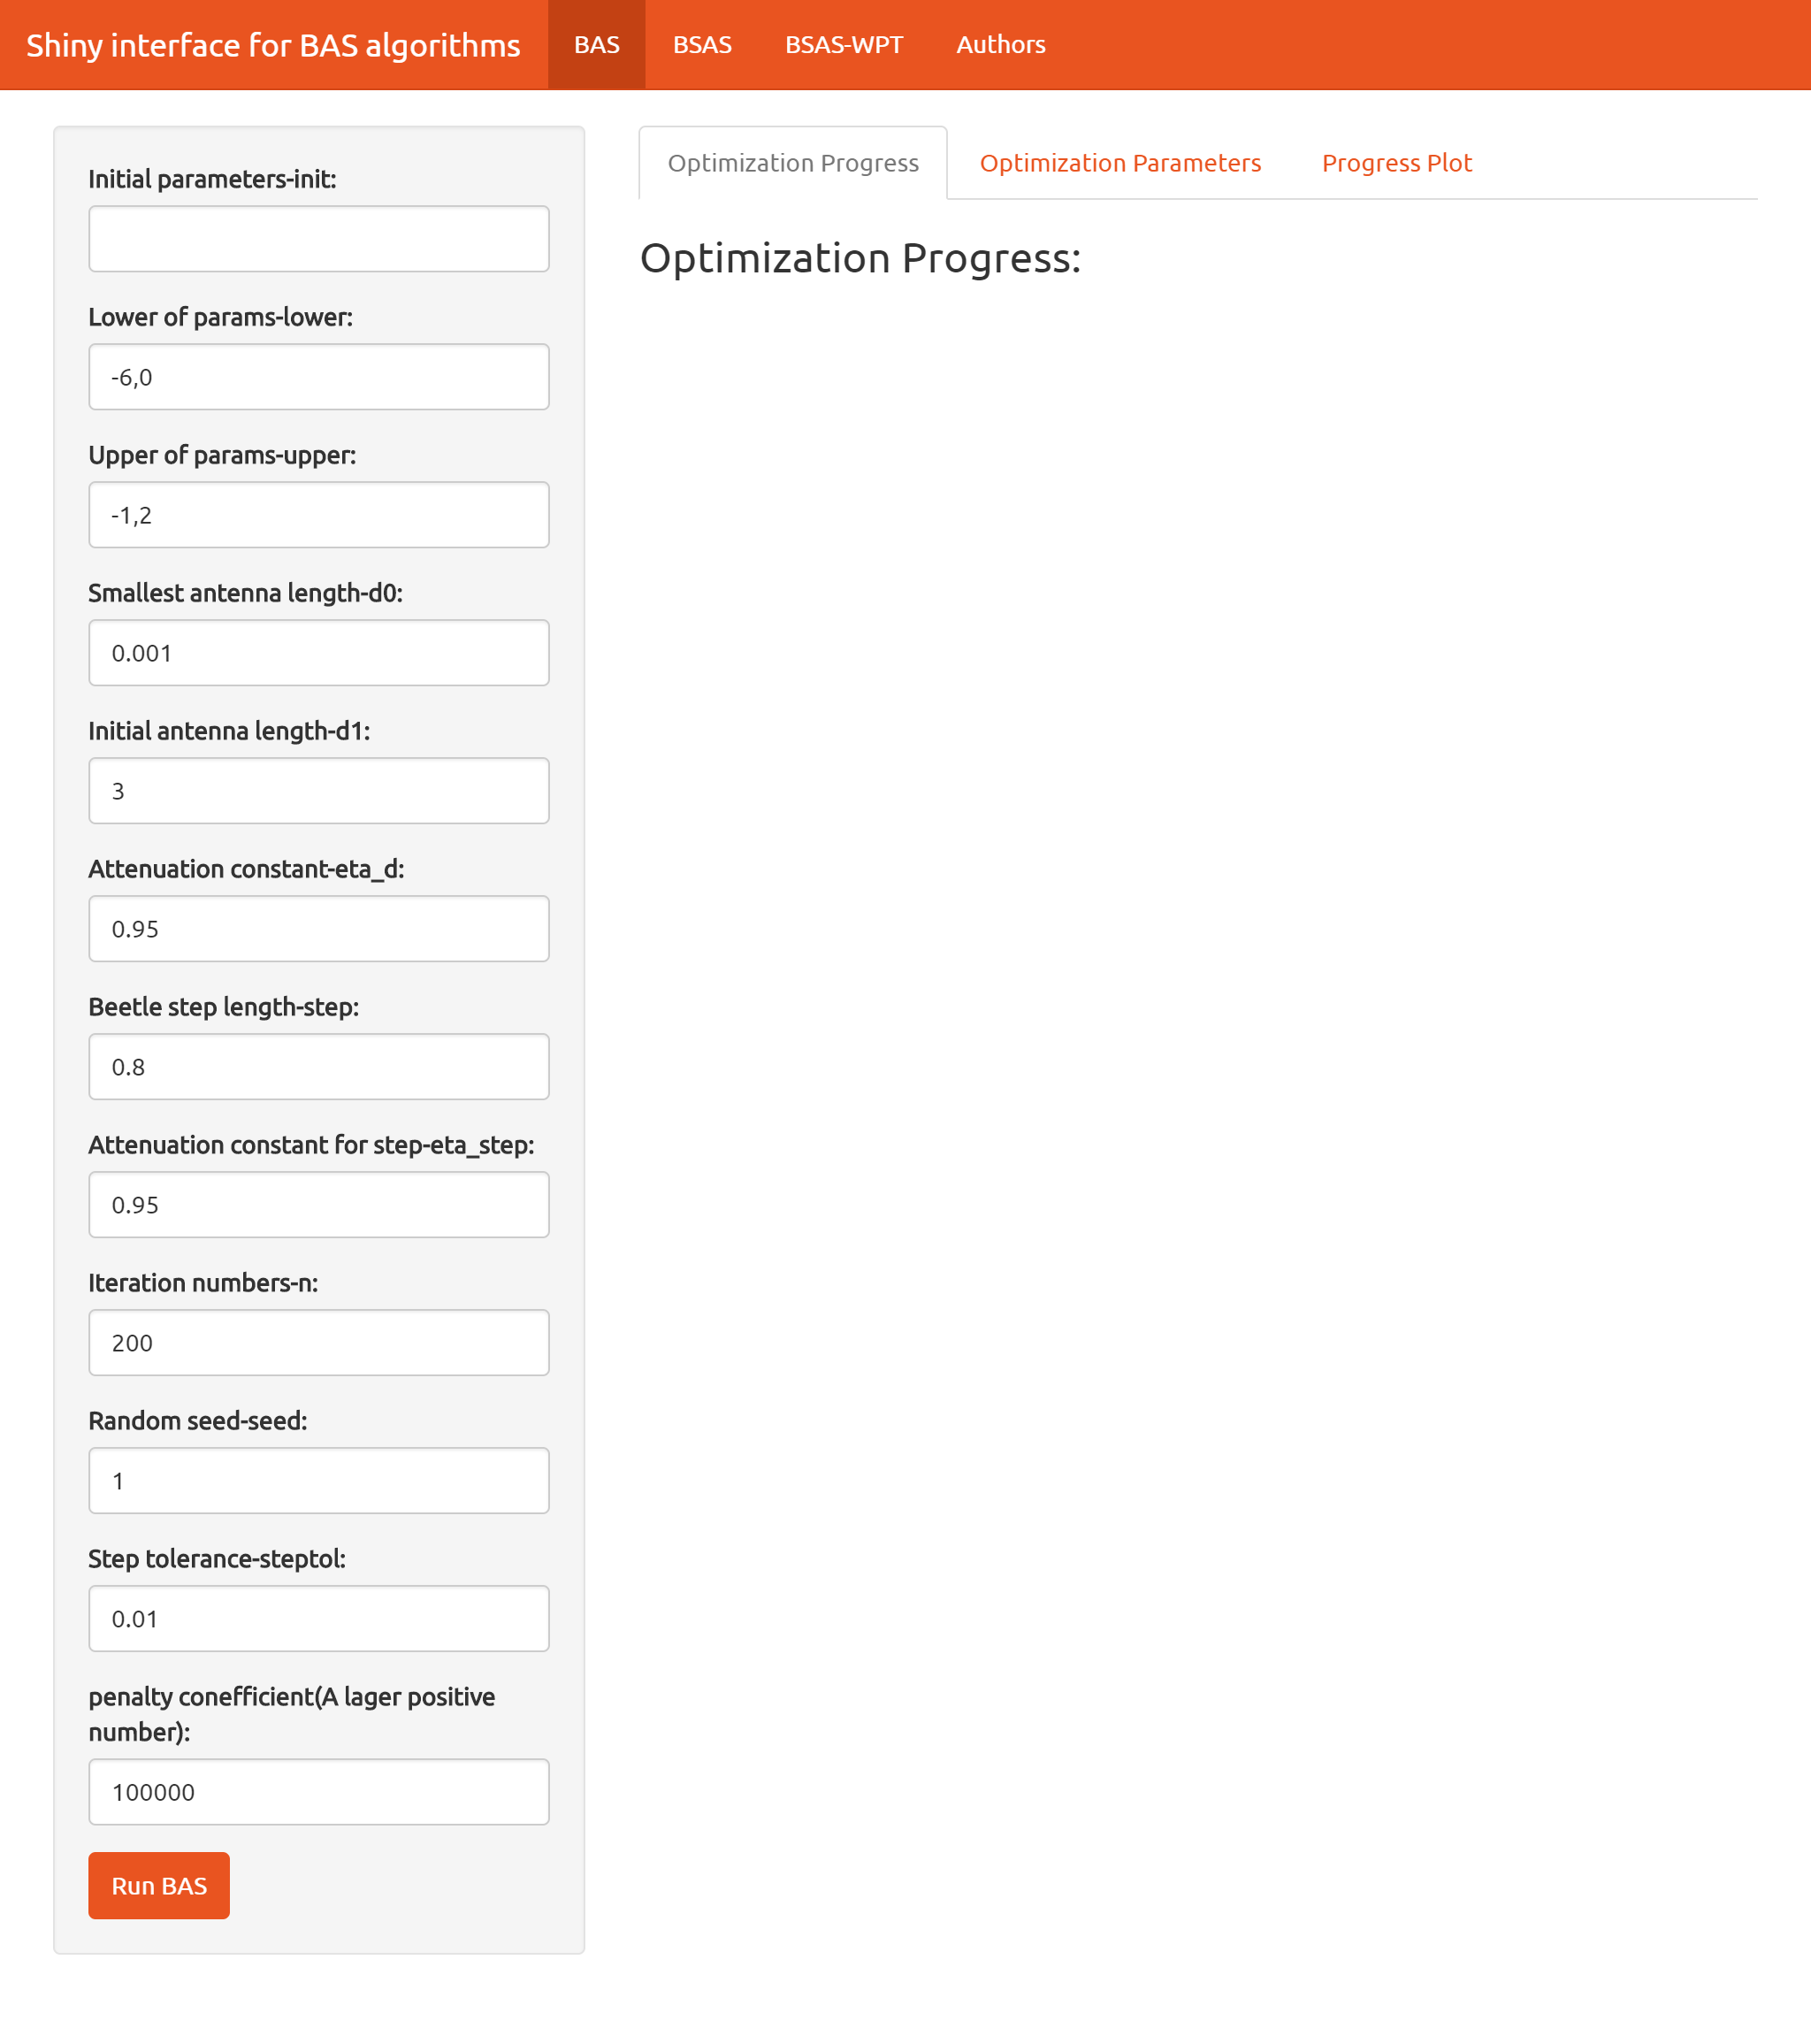
\includegraphics[width=0.95\linewidth]{img/app1} 

}

\caption{shiny interface}\label{fig:basapp}
\end{figure}

左边是固定的参数调节栏,最上方有目前的收录的三种算法可供选择,以及本包的作者信息。右侧也有三个选项,分别是\textbf{优化过程信息},\textbf{优化参数结果}以及\textbf{优化结果可视化}。

按照你的需要,调节好左边的参数信息(第一个参数,也就是初始值\texttt{init},默认为空,也可以指定),然后点击左下方的\texttt{Run\ BAS}键,即可看到如图\ref{fig:basprogress}的内容:

\begin{figure}

{\centering 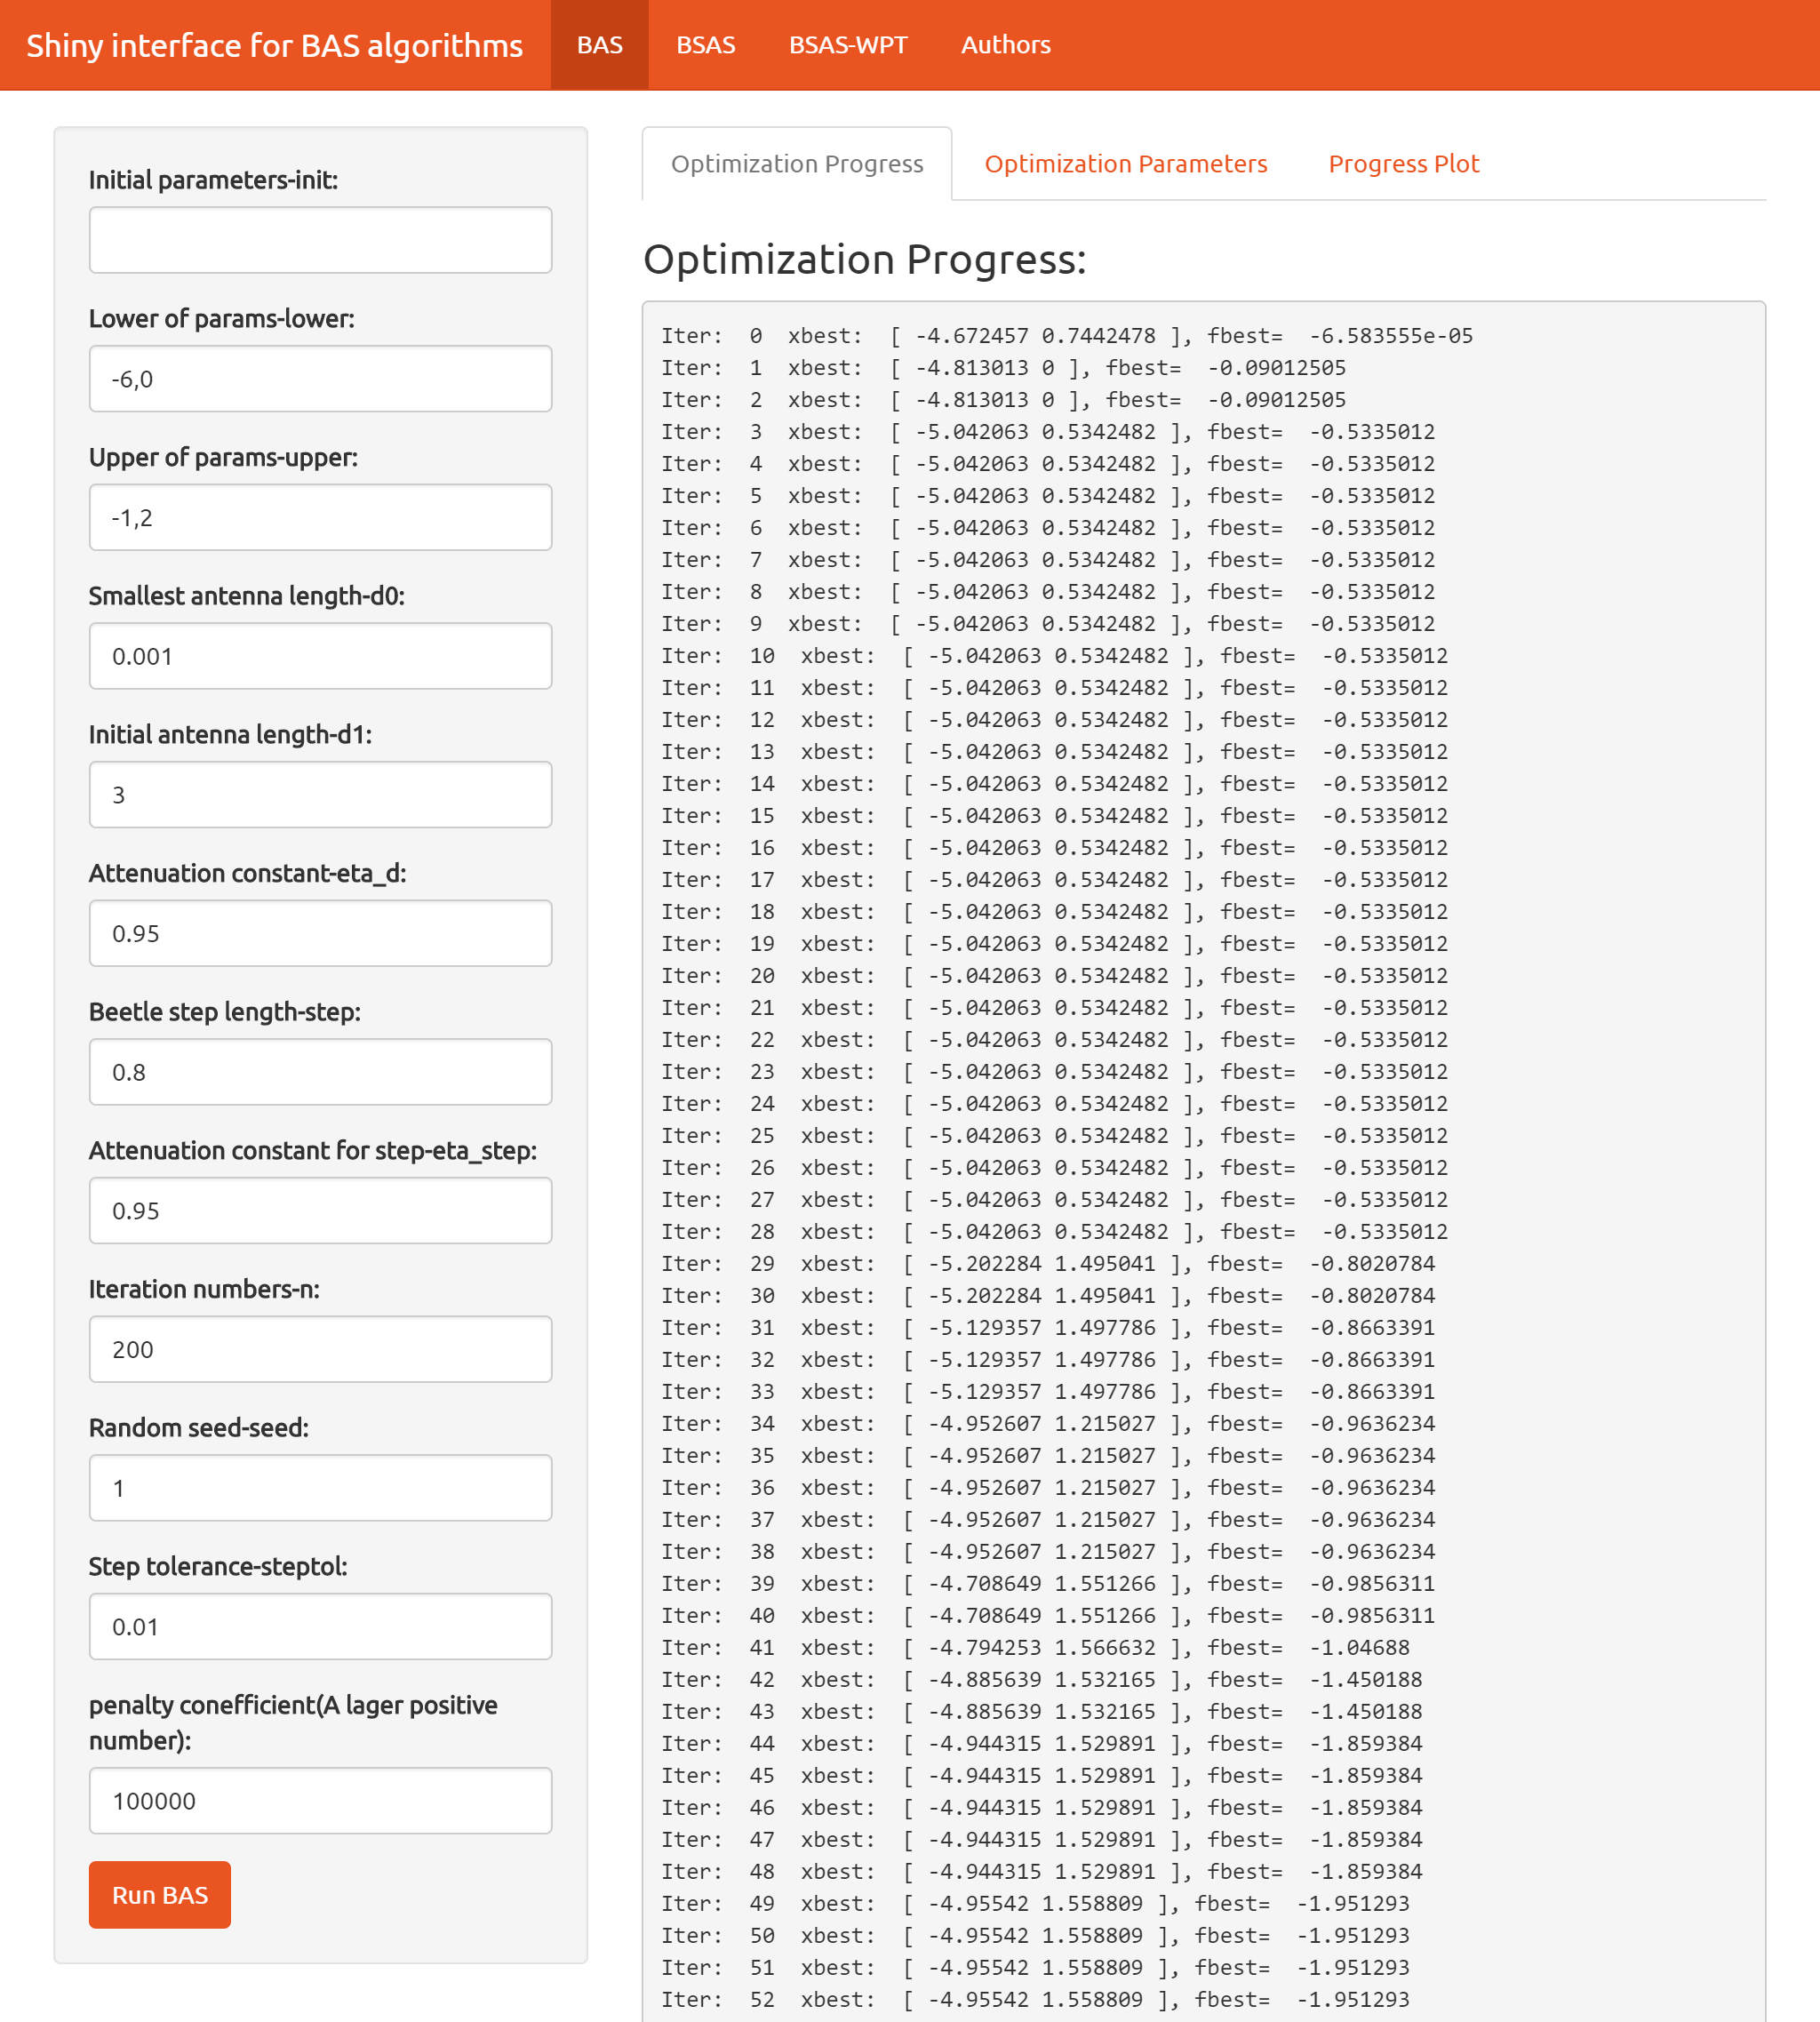
\includegraphics[width=0.95\linewidth]{img/app2} 

}

\caption{optimization progress栏信息}\label{fig:basprogress}
\end{figure}

\begin{quote}
由于回合数较大,因此只截取了部分内容显示。
\end{quote}

分别点击\texttt{Optimization\ Parameters}和\texttt{Progress\ Plot}键,可以看到最后的结果,以及可视化信息,分别如图\ref{fig:basparms}与
\ref{fig:basplot}所示。

\begin{figure}

{\centering 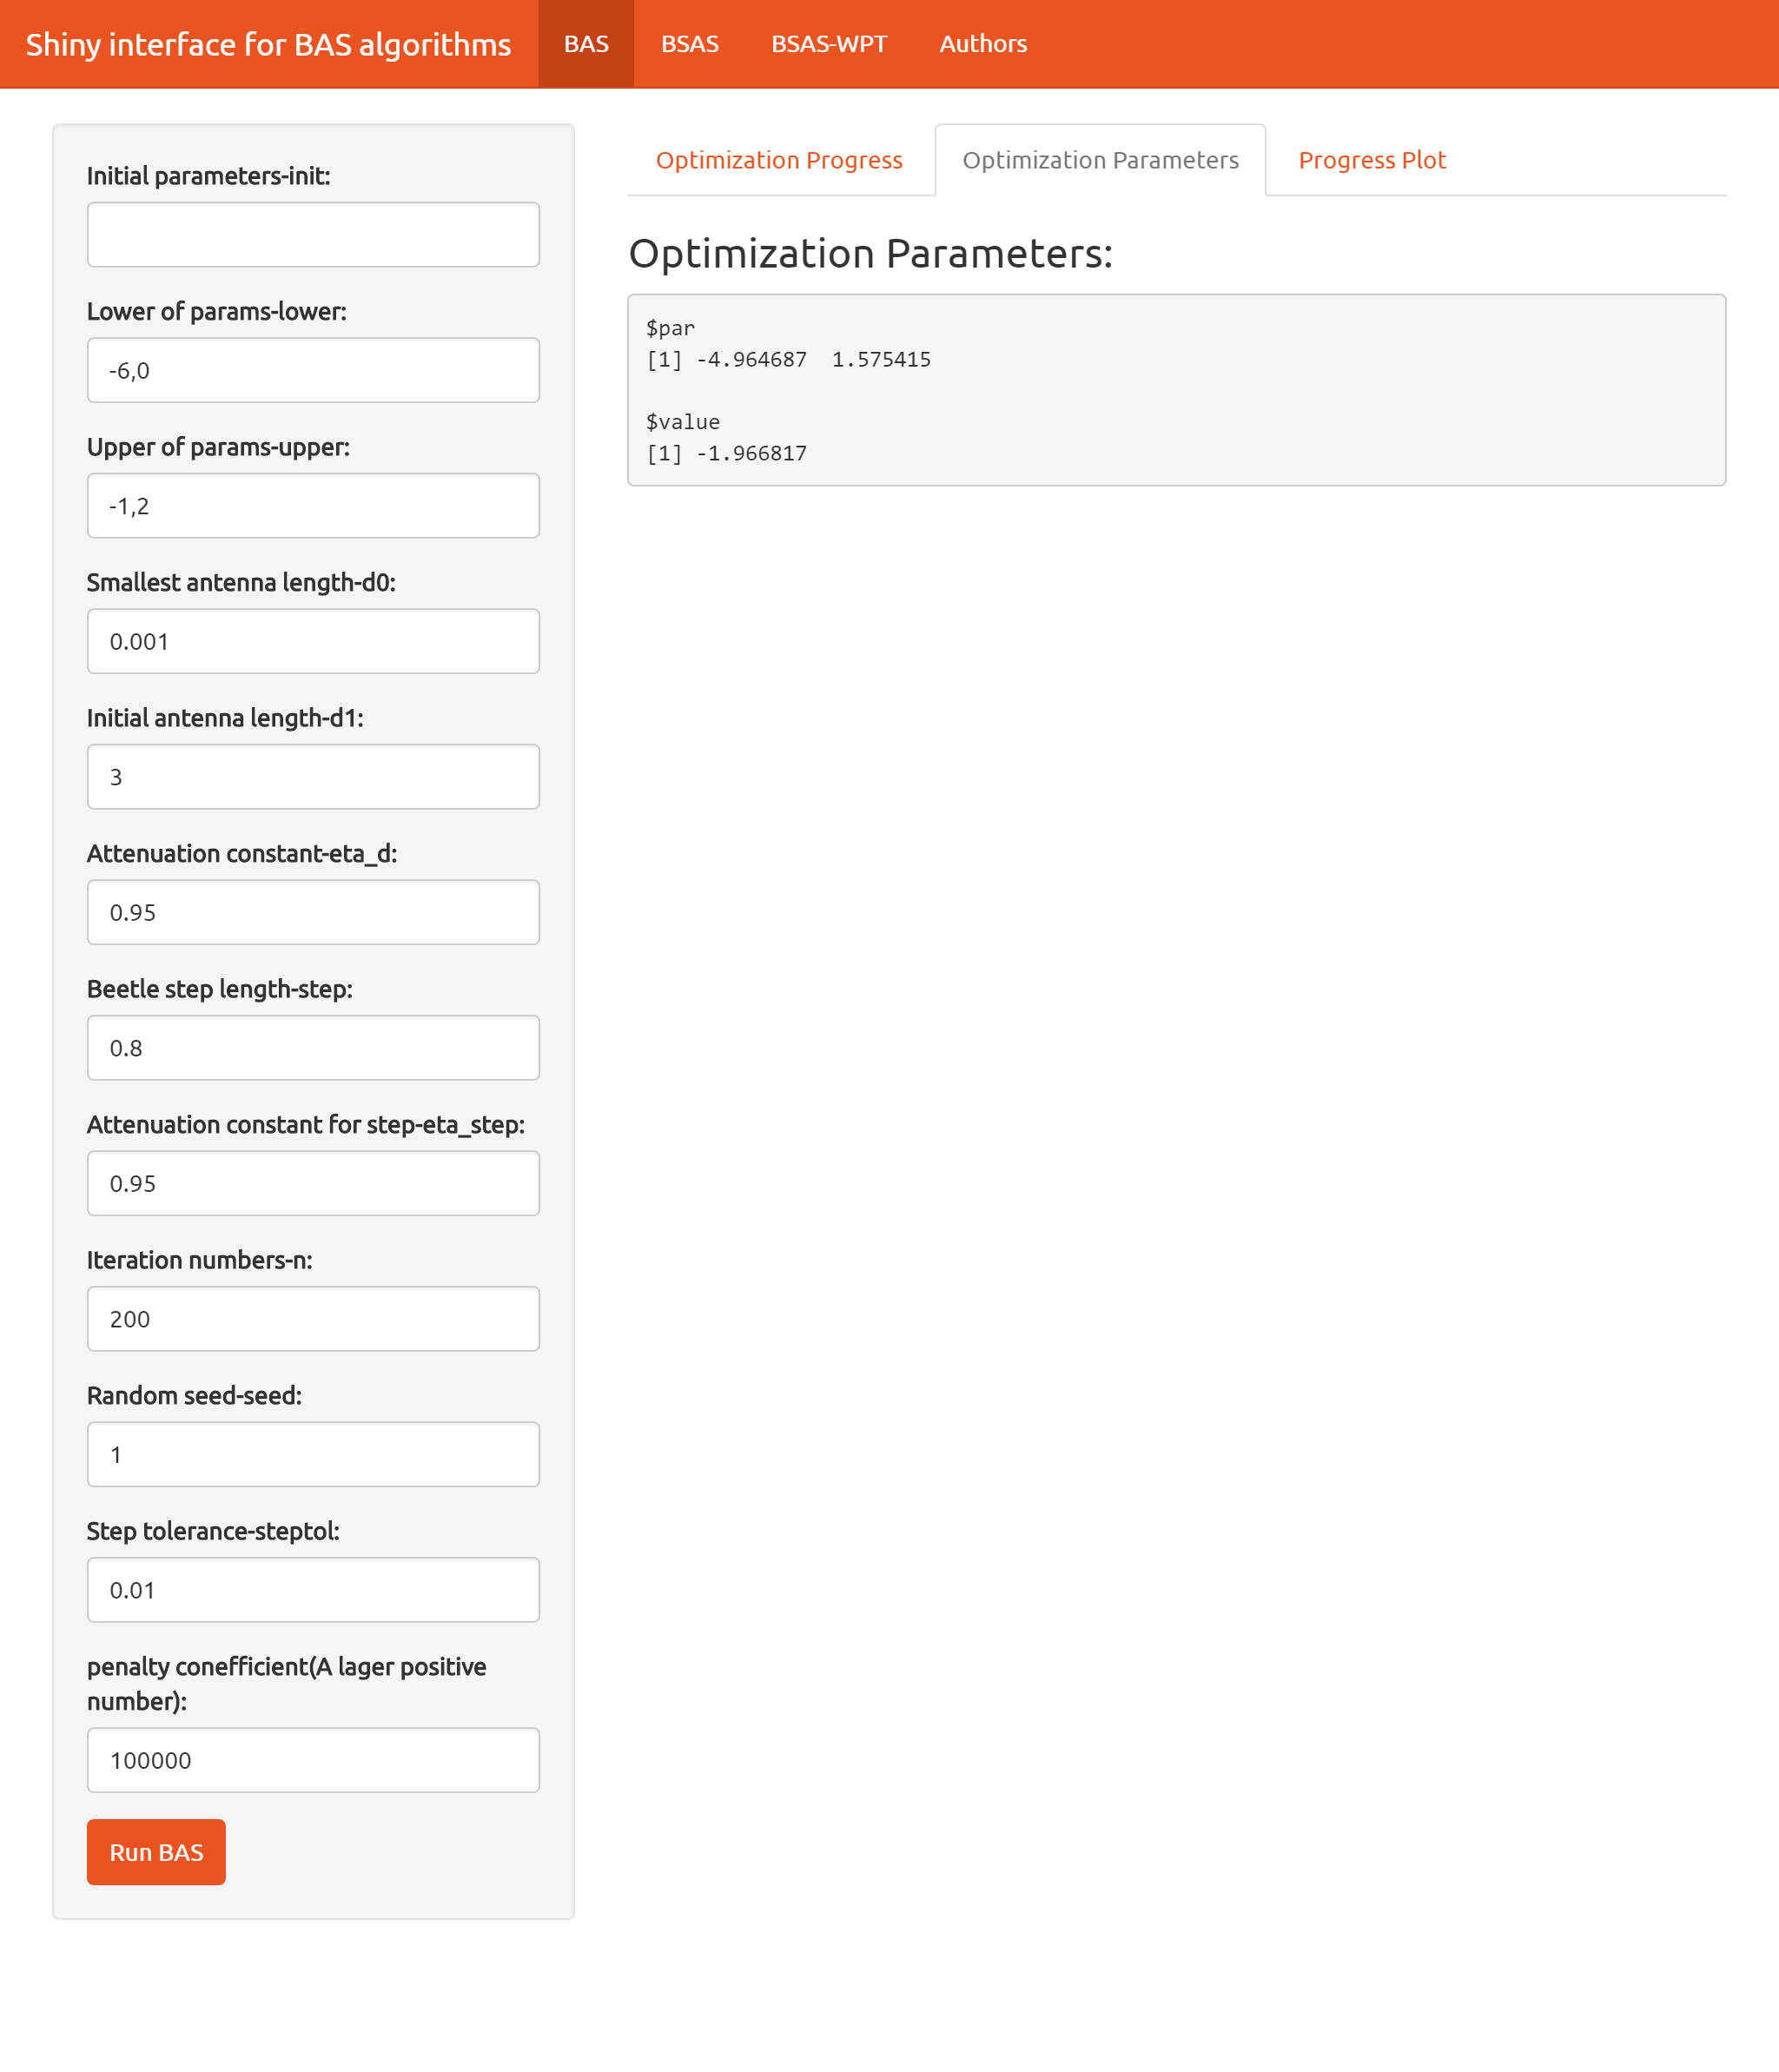
\includegraphics[width=0.95\linewidth]{img/app3} 

}

\caption{Optimization Parameters栏信息}\label{fig:basparms}
\end{figure}

可以看到,窗口的\texttt{\$par}显示的是参数的优化结果,而\texttt{\$value}则是对应的目标函数值。

\begin{figure}

{\centering 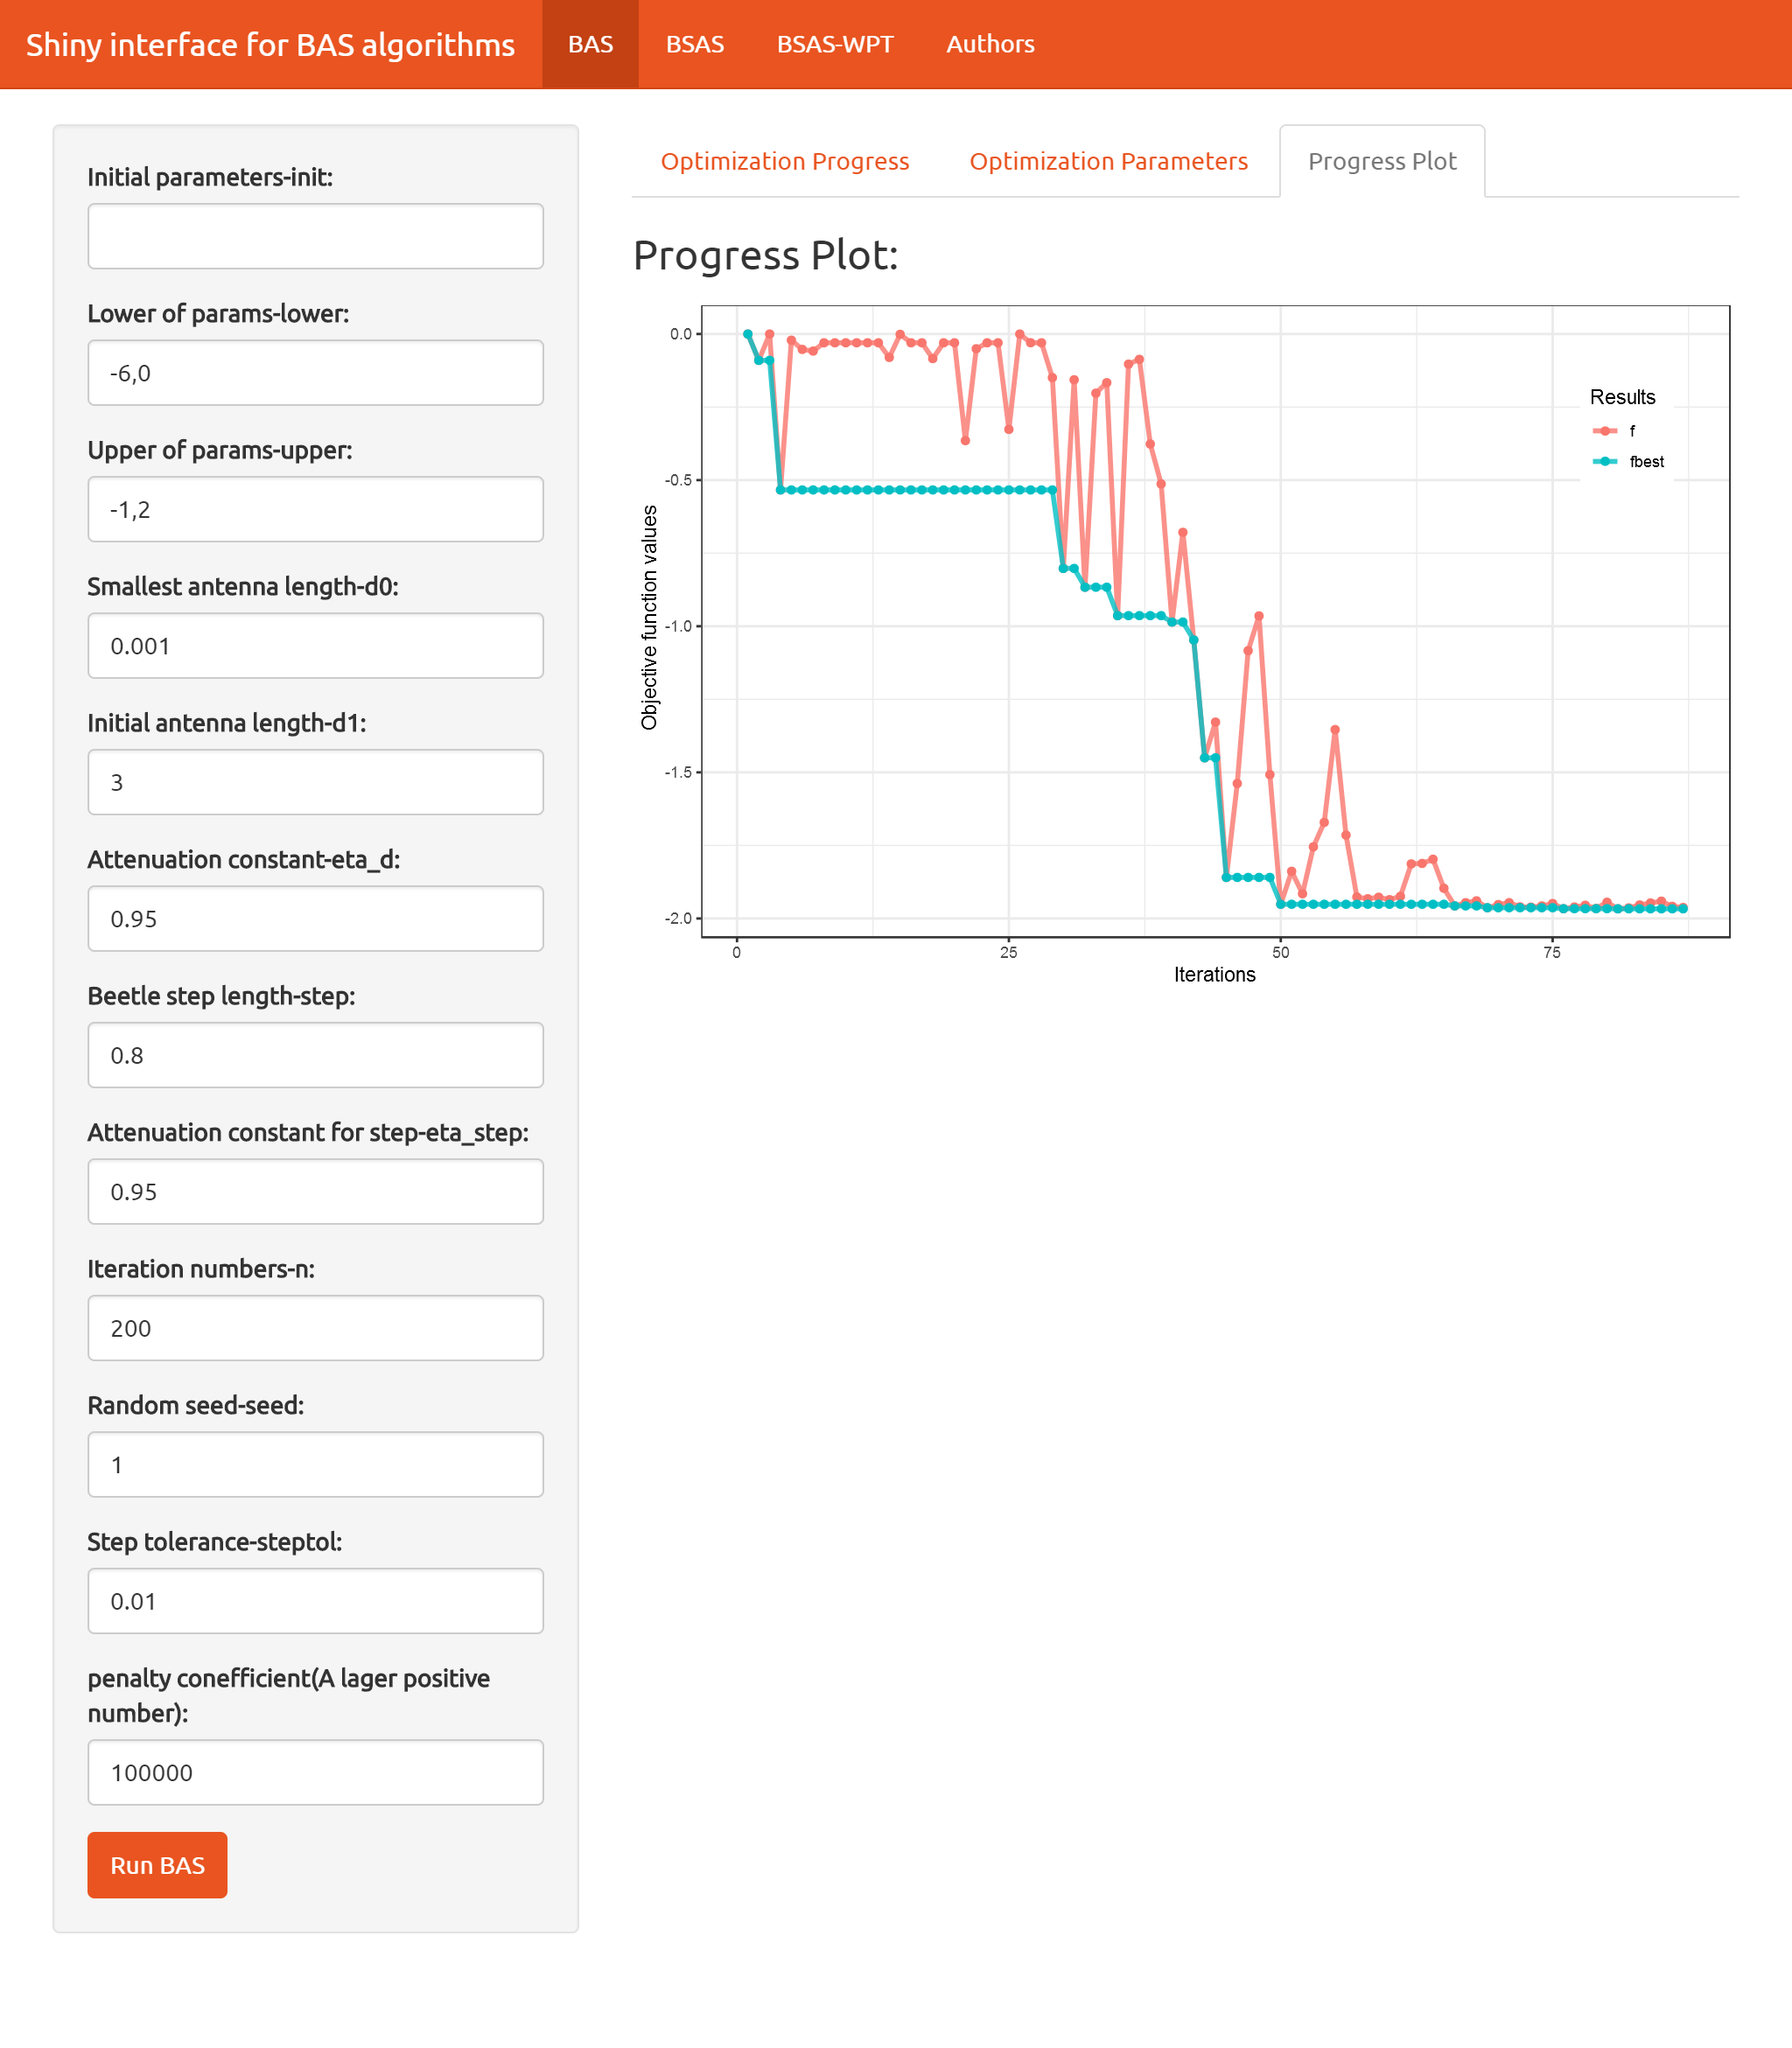
\includegraphics[width=0.95\linewidth]{img/app4} 

}

\caption{Progress Plot栏信息}\label{fig:basplot}
\end{figure}

\texttt{BAS}与其他两种算法有着不同的可视化结果,其并不是基于反馈来控制步长的。因此,图中的两条曲线,红色的为每一回合的目标函数值,而蓝色的为此前回合中最优的目标函数值。

\subsection{Pressure Vessel function}\label{pressure-vessel-function}

这次,我们在\texttt{BSAS-WPT}栏下进行界面使用。先在代码中预定义目标函数和约束:

\begin{Shaded}
\begin{Highlighting}[]
\NormalTok{pressure_Vessel <-}\StringTok{ }\KeywordTok{list}\NormalTok{(}
  \DataTypeTok{obj =} \ControlFlowTok{function}\NormalTok{(x)\{}
\NormalTok{    x1 <-}\StringTok{ }\KeywordTok{floor}\NormalTok{(x[}\DecValTok{1}\NormalTok{])}\OperatorTok{*}\FloatTok{0.0625}
\NormalTok{    x2 <-}\StringTok{ }\KeywordTok{floor}\NormalTok{(x[}\DecValTok{2}\NormalTok{])}\OperatorTok{*}\FloatTok{0.0625}
\NormalTok{    x3 <-}\StringTok{ }\NormalTok{x[}\DecValTok{3}\NormalTok{]}
\NormalTok{    x4 <-}\StringTok{ }\NormalTok{x[}\DecValTok{4}\NormalTok{]}
\NormalTok{    result <-}\StringTok{ }\FloatTok{0.6224}\OperatorTok{*}\NormalTok{x1}\OperatorTok{*}\NormalTok{x3}\OperatorTok{*}\NormalTok{x4 }\OperatorTok{+}\StringTok{ }
\StringTok{      }\FloatTok{1.7781}\OperatorTok{*}\NormalTok{x2}\OperatorTok{*}\NormalTok{x3}\OperatorTok{^}\DecValTok{2} \OperatorTok{+}
\StringTok{      }\FloatTok{3.1611}\OperatorTok{*}\NormalTok{x1}\OperatorTok{^}\DecValTok{2}\OperatorTok{*}\NormalTok{x4 }\OperatorTok{+}\StringTok{ }
\StringTok{      }\FloatTok{19.84}\OperatorTok{*}\NormalTok{x1}\OperatorTok{^}\DecValTok{2}\OperatorTok{*}\NormalTok{x3}
\NormalTok{  \},}
  \DataTypeTok{con =} \ControlFlowTok{function}\NormalTok{(x)\{}
\NormalTok{    x1 <-}\StringTok{ }\KeywordTok{floor}\NormalTok{(x[}\DecValTok{1}\NormalTok{])}\OperatorTok{*}\FloatTok{0.0625}
\NormalTok{    x2 <-}\StringTok{ }\KeywordTok{floor}\NormalTok{(x[}\DecValTok{2}\NormalTok{])}\OperatorTok{*}\FloatTok{0.0625}
\NormalTok{    x3 <-}\StringTok{ }\NormalTok{x[}\DecValTok{3}\NormalTok{]}
\NormalTok{    x4 <-}\StringTok{ }\NormalTok{x[}\DecValTok{4}\NormalTok{]}
    \KeywordTok{c}\NormalTok{(}
      \FloatTok{0.0193}\OperatorTok{*}\NormalTok{x3 }\OperatorTok{-}\StringTok{ }\NormalTok{x1,}\CommentTok{#<=0}
      \FloatTok{0.00954}\OperatorTok{*}\NormalTok{x3 }\OperatorTok{-}\StringTok{ }\NormalTok{x2,}
      \FloatTok{750.0}\OperatorTok{*}\FloatTok{1728.0} \OperatorTok{-}\StringTok{ }\NormalTok{pi}\OperatorTok{*}\NormalTok{x3}\OperatorTok{^}\DecValTok{2}\OperatorTok{*}\NormalTok{x4 }\OperatorTok{-}\StringTok{ }\DecValTok{4}\OperatorTok{/}\DecValTok{3}\OperatorTok{*}\NormalTok{pi}\OperatorTok{*}\NormalTok{x3}\OperatorTok{^}\DecValTok{3}
\NormalTok{    )}
\NormalTok{  \}}
\NormalTok{)}
\end{Highlighting}
\end{Shaded}

调用用户界面,注意此时多出了\texttt{constr},也就是约束函数,\texttt{\$}符号在索引列表中的元素时使用:

\begin{Shaded}
\begin{Highlighting}[]
\KeywordTok{run_BAS_App}\NormalTok{(}\DataTypeTok{func =}\NormalTok{ pressure_Vessel}\OperatorTok{$}\NormalTok{obj,}
            \DataTypeTok{constr =}\NormalTok{ pressure_Vessel}\OperatorTok{$}\NormalTok{con)}
\end{Highlighting}
\end{Shaded}

自行调整参数后,用户界面如图\ref{fig:wpt1}所示:

\begin{figure}

{\centering 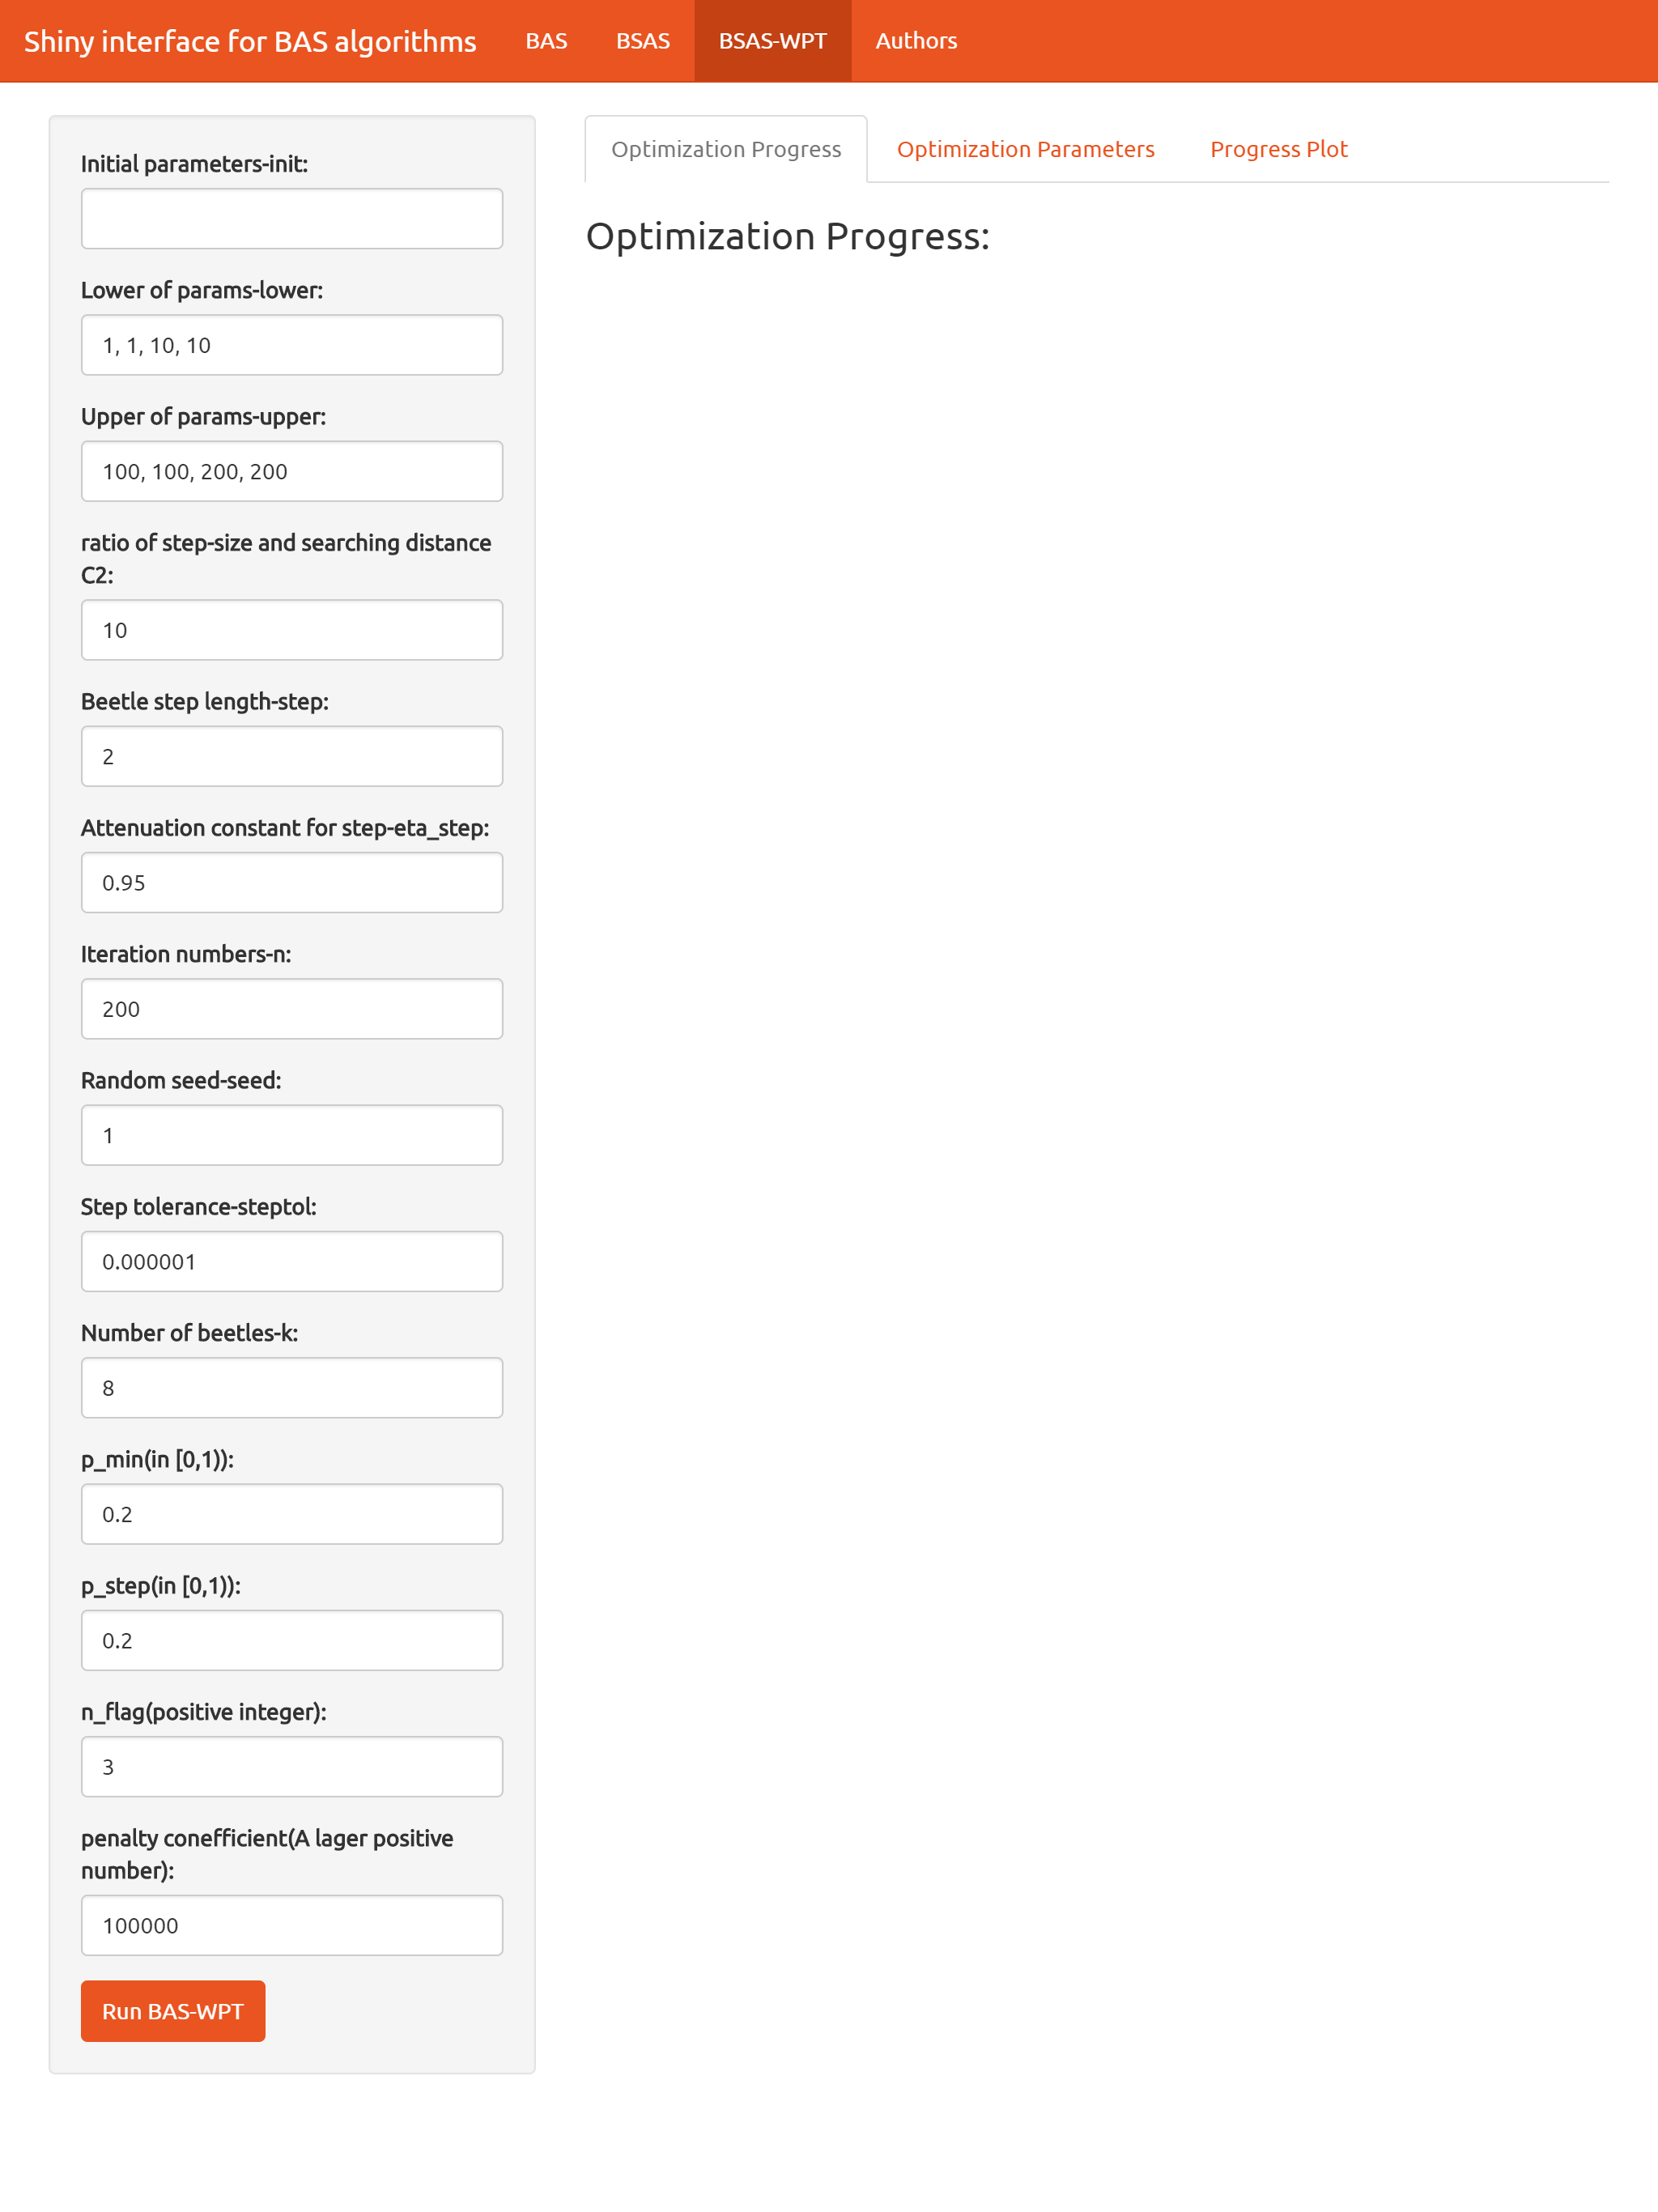
\includegraphics[width=0.95\linewidth]{img/wpt1} 

}

\caption{BSAS-WPT参数调整}\label{fig:wpt1}
\end{figure}

点击\texttt{Run\ BAS-WPT}之后,选择\texttt{optimization\ Parameters}栏目,可以看到优化结果如图\ref{fig:wptparms}所示:

\begin{figure}

{\centering 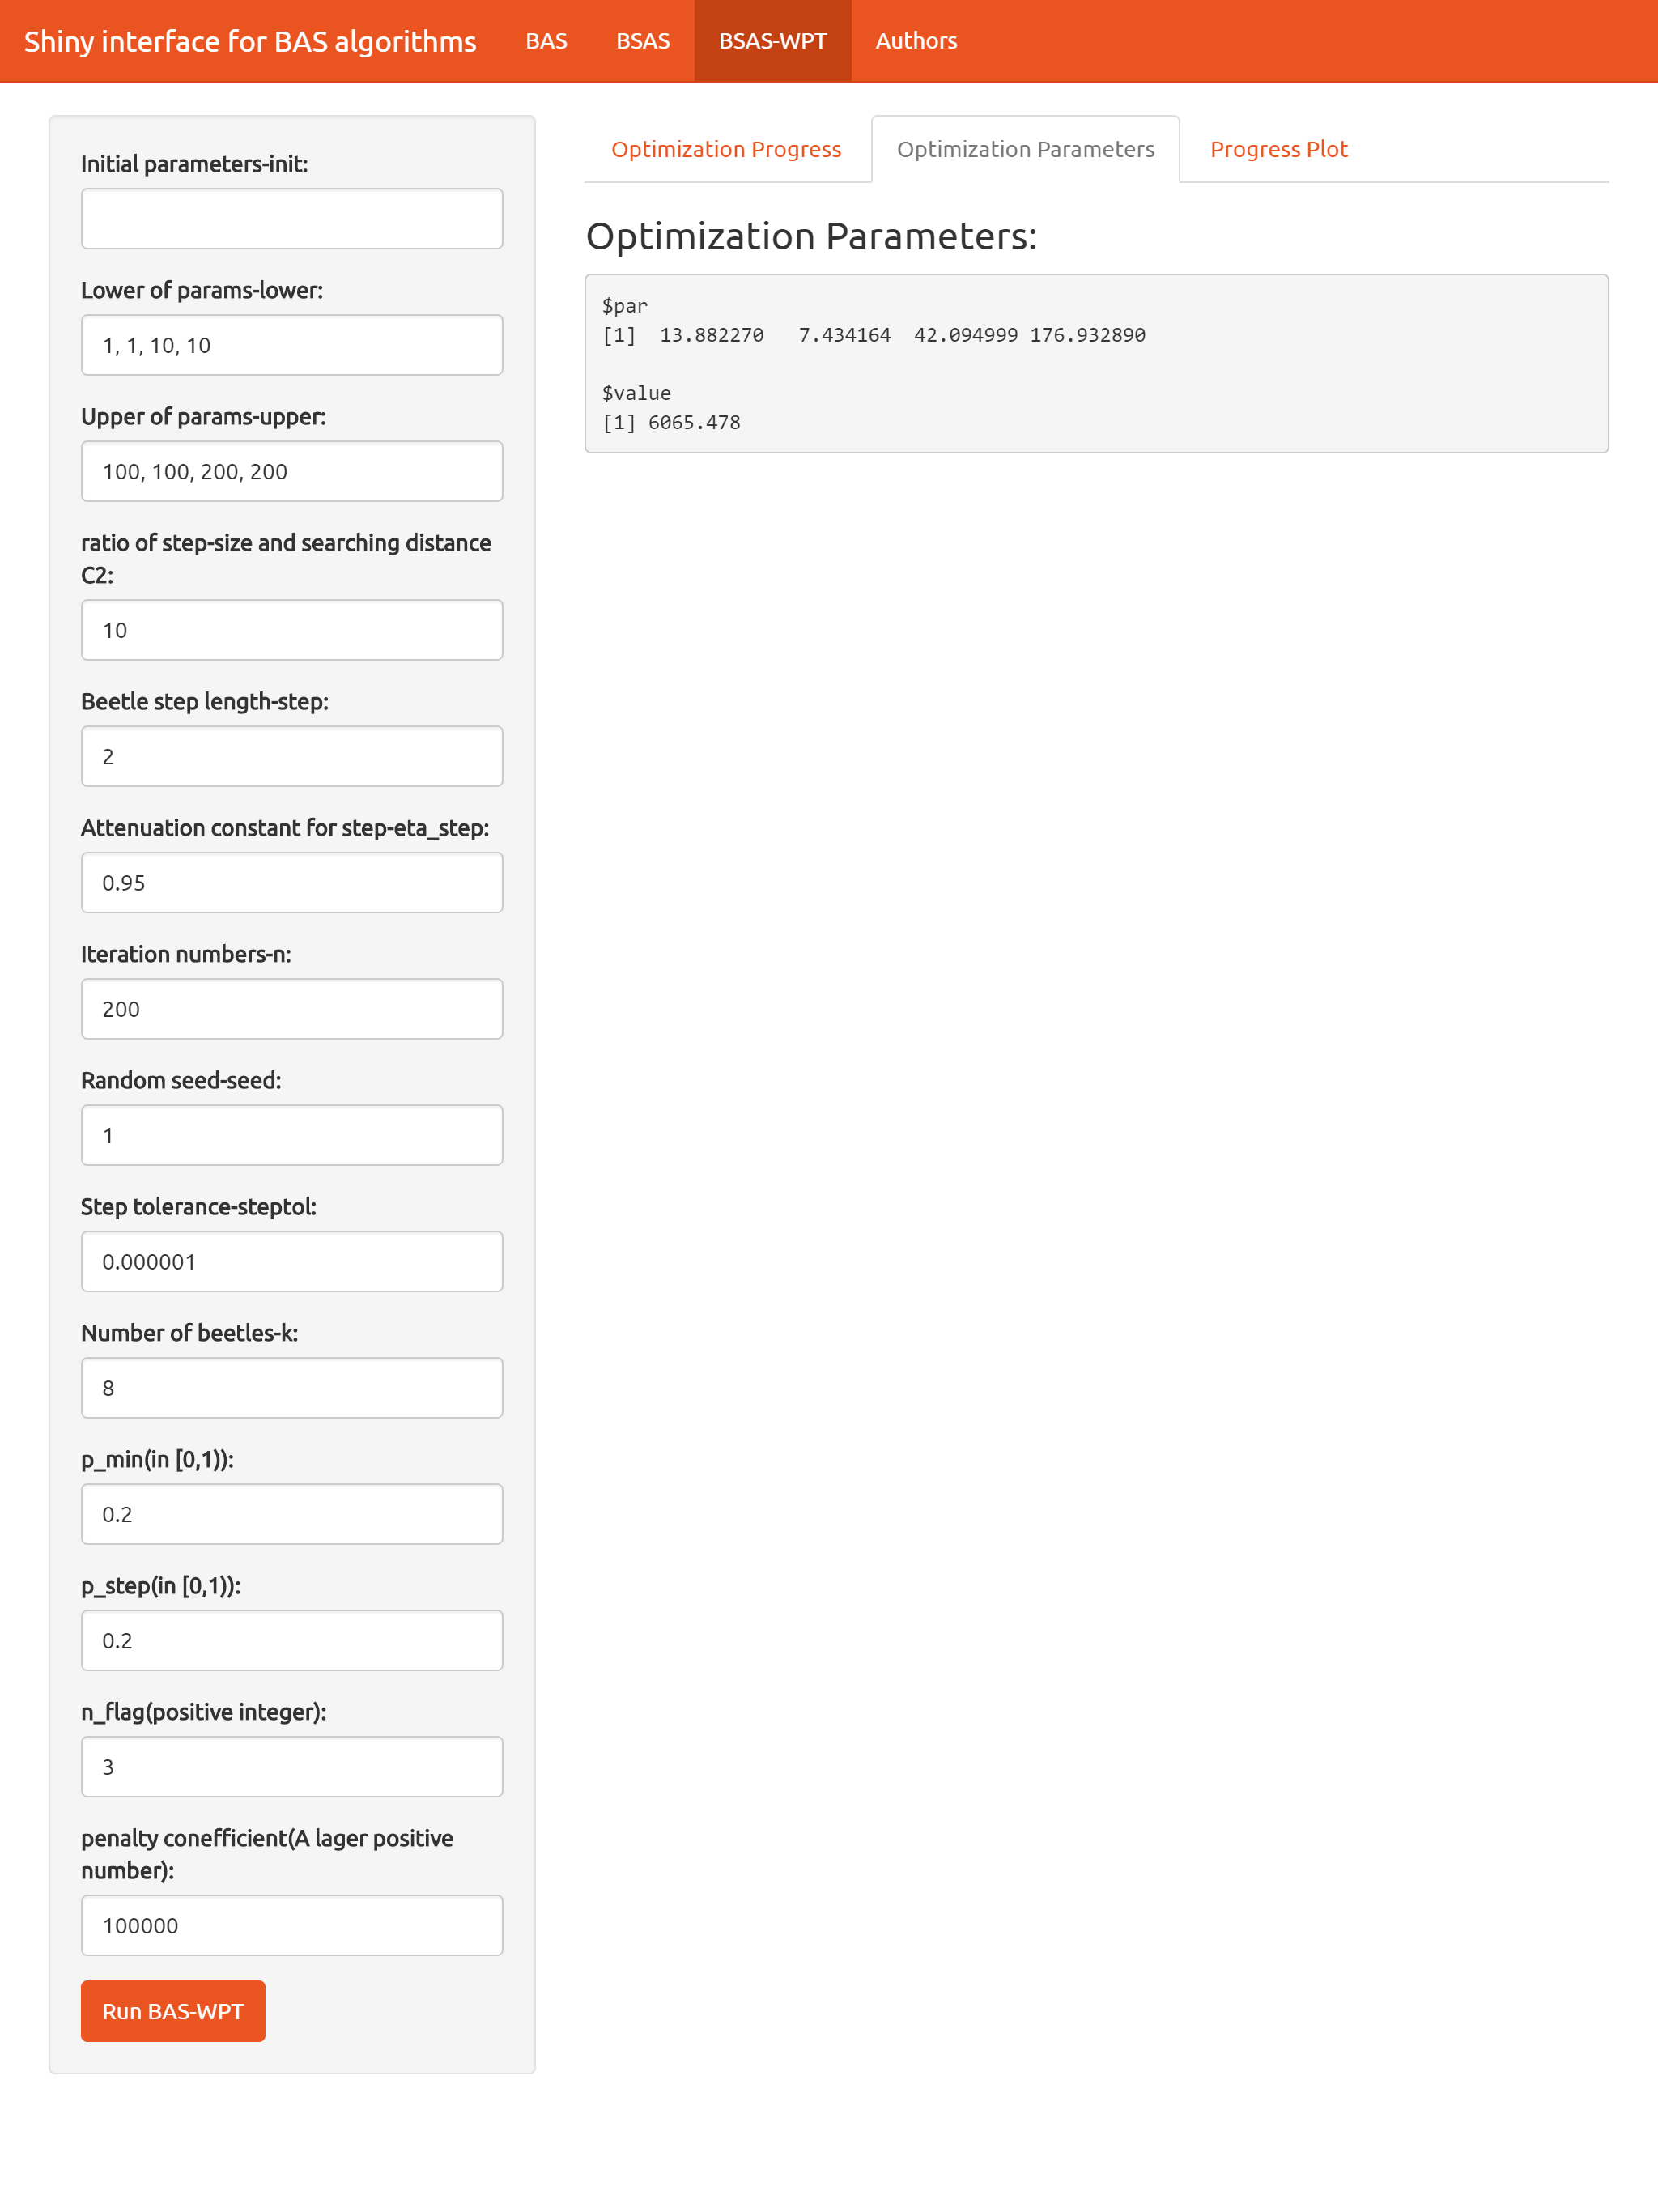
\includegraphics[width=0.95\linewidth]{img/wpt2} 

}

\caption{BSAS-WPT优化结果}\label{fig:wptparms}
\end{figure}

选择\texttt{Progress\ Plot}栏目,过程可视化如图\ref{fig:wptplot}所示:

\begin{figure}

{\centering 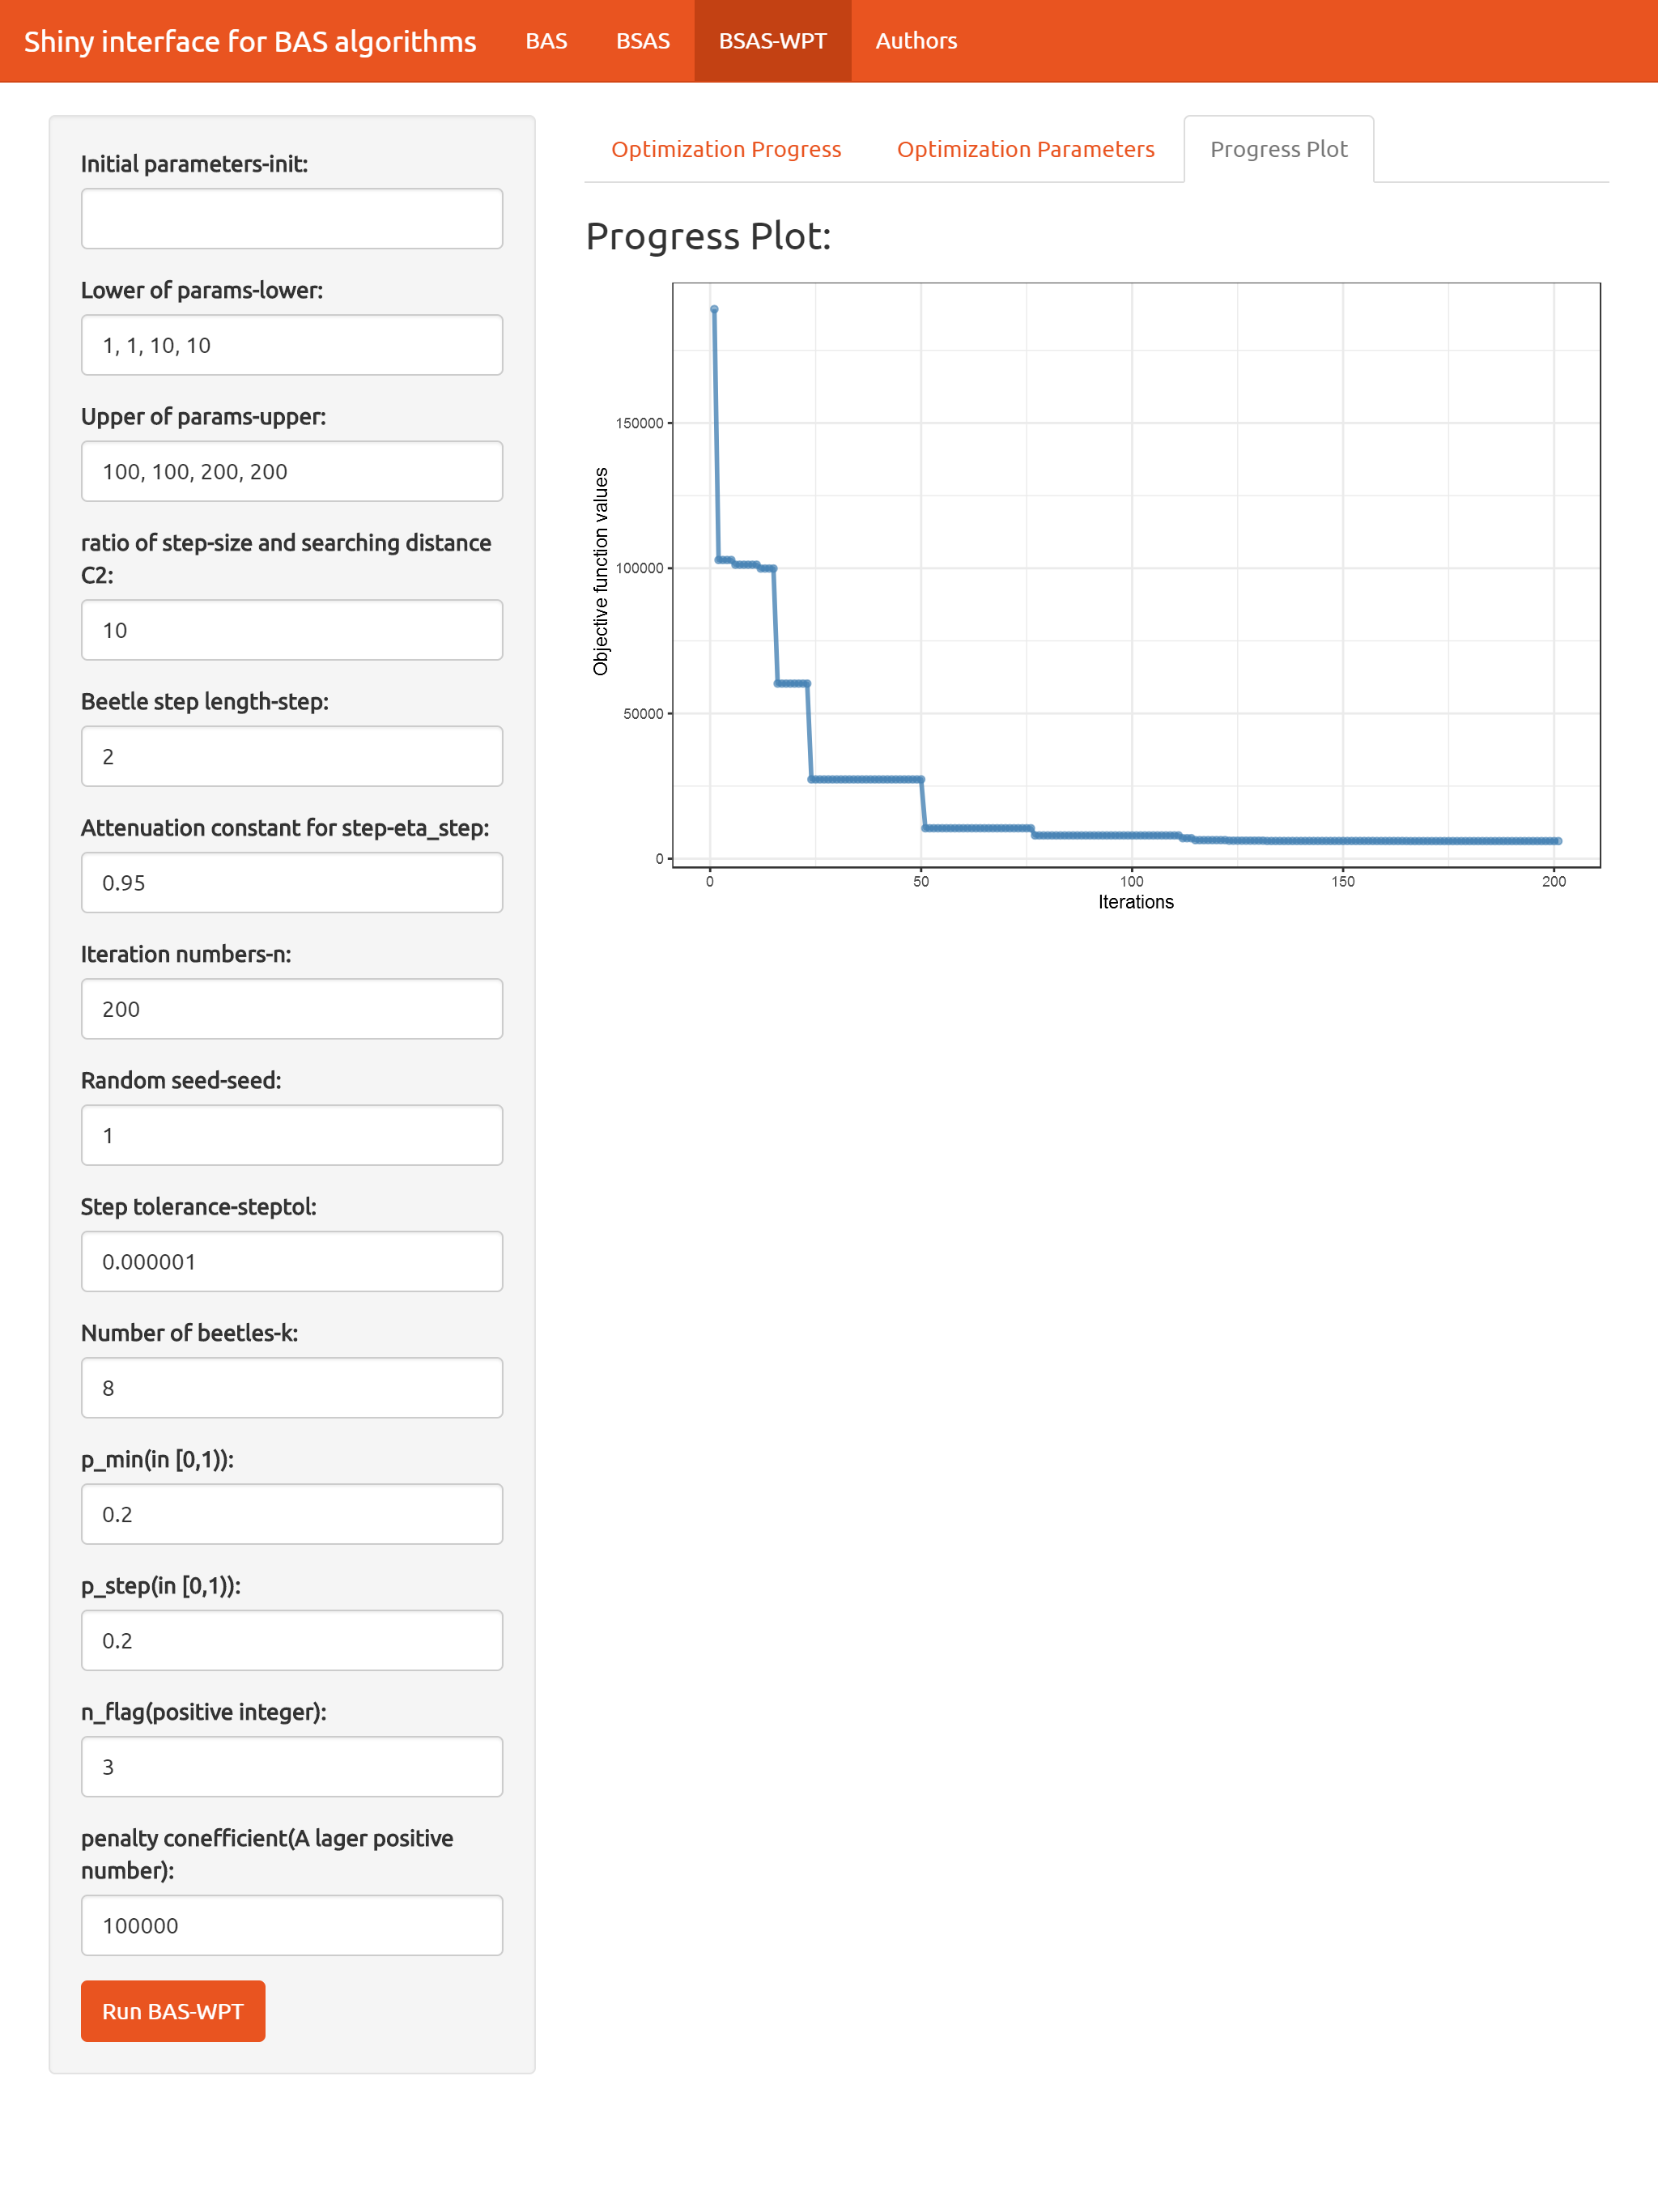
\includegraphics[width=0.95\linewidth]{img/wpt3} 

}

\caption{BSAS-WPT优化过程可视化}\label{fig:wptplot}
\end{figure}

\section{Authors界面}\label{authors}

如果并不想执行任何函数优化,则可以不指定函数和约束。在\texttt{R}里面输入以下代码:

\begin{Shaded}
\begin{Highlighting}[]
\KeywordTok{library}\NormalTok{(rBAS) }\CommentTok{#加载rBAS包}
\KeywordTok{run_BAS_App}\NormalTok{() }\CommentTok{#直接调用函数}
\end{Highlighting}
\end{Shaded}

可以看到\texttt{rBAS}的用户界面,里面有关于\texttt{rBAS}的作者信息,如图\ref{fig:author}所示。

\begin{figure}

{\centering 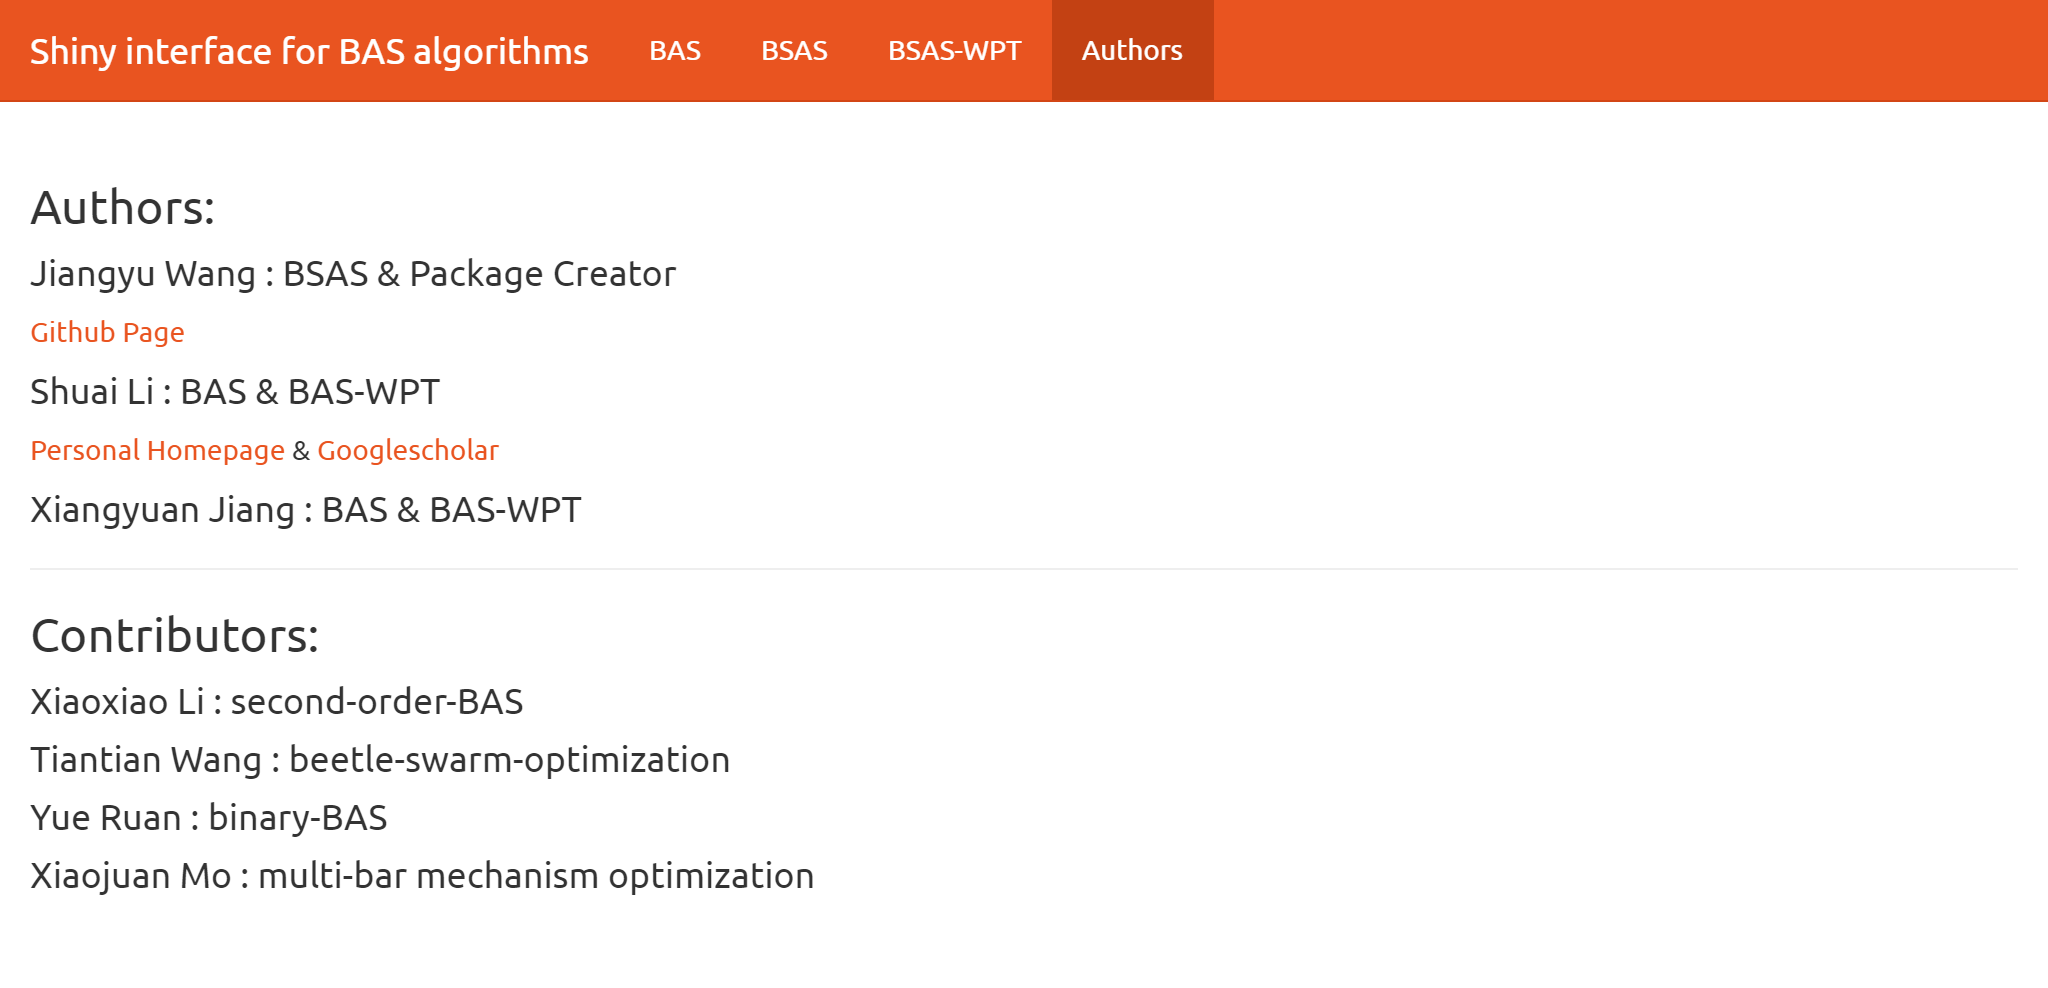
\includegraphics[width=1\linewidth]{img/author} 

}

\caption{用户界面作者信息}\label{fig:author}
\end{figure}

如果大家对该项目有兴趣,参与了包的开发,或者\texttt{BAS}算法应用案例的提出。我会在征得当事人同意的情况下,将名字加入该界面:)。

\chapter{BAS案例一:多杆机构优化问题}\label{examples}

说明:由于自身专业知识局限,在整理转述各位研究者或贡献者所提供的材料时,我可能无法准确地表达出对应领域的知识要点。避免言多必失,我仅仅做简要的翻译或者是介绍。对于读者而言,如果觉得并不能解你之疾,或没有\textbf{挠到痒处},建议直接和对应的作者联系。对于贡献者而言,如果我表述有误,欢迎提出建议,或者在github上\texttt{pull\ request}。

\begin{quote}
由群友莫小娟博士研究生提供案例。
\end{quote}

由于案例均为各位热心的同学提供,均为自己的研究。因此,希望大家要引用其中的结果时,可以引用对应同学的文章。此外,也请大家转载时注明来源。

\section{背景}

\subsection{四连杆机构(Four-bar linkage mechanism)}\label{bars4}

四连杆机构如图\ref{fig:fourbars}所示:

\begin{figure}

{\centering 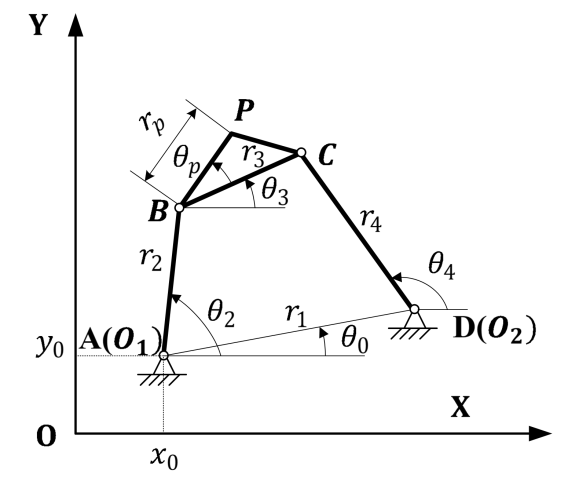
\includegraphics[width=0.7\linewidth]{img/bars4} 

}

\caption{四连杆机构示意}\label{fig:fourbars}
\end{figure}

基于闭环矢量方程,推导出节点位置。推导过程如式\eqref{eq:bars4loop1}至式\eqref{eq:bars4loop4}:

\begin{equation}
\mathbf{\text{Loop:}}   r_1e^{i\theta_0} + r_4e^{i\theta_4} - r_2e^{i\theta_2} -r_3e^{i\theta_3} = 0\\
\label{eq:bars4loop1}
\end{equation}

\begin{equation}
\begin{cases} 
r_1cos(\theta_0) + r_4cos(\theta_4)-r_2cos(\theta_2)-r_3cos(\theta_3)=0 \\ 
r_1sin(\theta_0) + r_4sin(\theta_4)-r_2sin(\theta_2)-r_3sin(\theta_3)=0
\end{cases}
\label{eq:bars4loop2}
\end{equation}

\begin{equation}
\begin{split}
&\theta_3 =2atan(\frac{-A\pm\sqrt{2}{A^2-4BC}}{2B})+\theta_0\\
&A = cos(\theta_2 - \theta_0)-K_1+K_2cos(\theta_2-\theta_0)+K_3\\
&B = -2sin(\theta_2-\theta_0), F=K_1+(K_2-1)cos(\theta_2-\theta_0)+K_3\\
&K_1 = r_1/r_2,K_2=r_1/r_3,K_3=(r_4^2-r_1^2-r_2^2-r_3^2)/(2r_2r_3)\\
\end{split}
\label{eq:bars4loop3}
\end{equation}

\begin{equation}
\begin{cases} 
x_p=x_0+r_2cos(\theta_2)+r_pcos(\theta_3+\theta_p) \\ 
y_p=y_0+r_2sin(\theta_2)+r_psin(\theta_3+\theta_p)
\end{cases}
\label{eq:bars4loop4}
\end{equation}

\subsection{六连杆机构(Stephenson III Six-bar linkage
mechanism)}\label{bars6}

六连杆机构如图\ref{fig:sixbars}所示:

\begin{figure}

{\centering 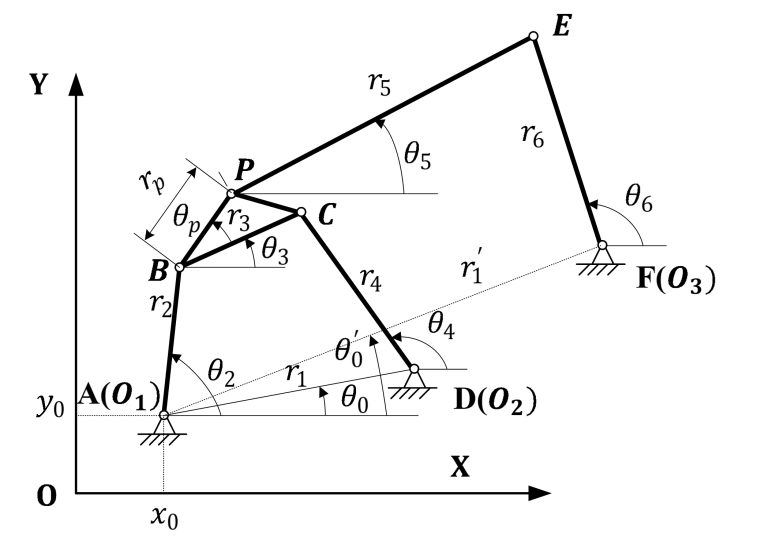
\includegraphics[width=0.7\linewidth]{img/bars6} 

}

\caption{六连杆机构示意}\label{fig:sixbars}
\end{figure}

基于闭环矢量方程,推导出节点位置和外部链接角度。推导过程如式\eqref{eq:bars6loop1}至式\eqref{eq:bars6loop2}:

\begin{equation}
\begin{split}
&\mathbf{\text{Loop1:}}   r_1e^{i\theta_0} + r_4e^{i\theta_4} - r_2e^{i\theta_2} -r_3e^{i\theta_3} = 0\\
&\mathbf{\text{Loop2:}}   r_1'e^{i\theta_0'} + r_6e^{i\theta_6} - r_2e^{i\theta_2} -r_pe^{i(\theta_3+\theta_p)}-r_5e^{i\theta_5} = 0\\
\end{split}
\label{eq:bars6loop1}
\end{equation}

\begin{equation}
\begin{split}
\text{Loop1:}\\
&\alpha = r_2cos(\theta_2) - r_1cos(\theta_0), \beta = r_2sin(\theta_2)-r_1sin(\theta_0) \\
&\gamma = (r_4^2+\alpha^2+\beta^2-r_3^2)/(2r_4),\lambda=atan2(\alpha,\beta)\\
&\theta_4 = atan(cos(\lambda)\gamma/\beta,\{1-(cos(\lambda)\gamma/\beta)^2\}^{1/2})-\lambda\\
&\theta_3=atan2(r_4sin(\theta_4)-\beta,r_4cos(\theta_4)-\alpha)\\
\text{Loop2:}\\
&\alpha_1 = r_2cos(\theta_2)+r_pcos(\theta_3+\theta_p)-r_6cos(\theta_6)\\
&\beta_1=r_2sin(\theta_2)+r_psin(\theta_3+\theta_p)-r_6sin(\theta_6)\\
&\gamma_1=(r_6^2+\alpha_1^2+\beta_1^2-r_5^2)/(2r_6),\lambda_1=atan2(\alpha_1,\beta_1)\\
&\theta_6=atan2(cos(\lambda)\gamma_1/\beta_1,-\{1-(cos(\lambda_1)\gamma_1/\beta_1)^{2}\}^{1/2}) - \lambda_1\\
&\theta_5 = atan2(r_6sin(\theta_6)-\beta_1,r_6cos(\theta_6)-\alpha_1)
\end{split}
\label{eq:bars6loop2}
\end{equation}

于是,可以得到节点位置如式\eqref{eq:bars6loop3}:

\begin{equation}
\begin{cases} 
x_A = x_0,y_A = y_0 \\
x_D = x_0+r_1cos(\theta_0),y_D = y_0+r_1sin(\theta_0)\\
x_F = x_0+r_1'cos(\theta_0'),x_F = x_0 + r_1'sin(\theta_0')\\
x_p = x_0 + r_2cos(\theta_2) + r_pcos(\theta_3+\theta_p)\\
y_P = y_0 + r_2sin(\theta_2)+r_Psin(\theta_3+\theta_p)\\
\end{cases}
\label{eq:bars6loop3}
\end{equation}

\section{优化问题}

\subsection{四连杆机构}\label{bars4optim}

四杆机构的优化问题可以用式\eqref{eq:optim4bars}表示。

\begin{equation}
\begin{split}
\text{min   } &\sum_{i=1}^N[(P_{Xd}^i-P_X^i)^2+(P_{Yd}^i-P_Y^i)^2]+M_1h_1(x)+M_2h_2(x)\\
\text{where } & x_i\in [l_{min}^i,l_{max}^i] \quad \forall x_i \in X,\\
&X=[r_1,r_2,r_3,r_4,r_p,\theta_p,\theta_0,x_0,y_0,\theta_2^1,\cdots,\theta_2^N]\\
\end{split}
\label{eq:optim4bars}
\end{equation}

其中,

\begin{equation}
h_1(x) = \begin{cases}
1, & \text{the Grashof condition false}\\
0, & \text{the Grashof condition true}
\end{cases}
\label{eq:hx1}
\end{equation}

\begin{equation}
h_2(x) = \begin{cases}
1, & \text{the sequence condition of the crank angle false}\\
0, & \text{the sequence condition of the crank angle true}
\end{cases}
\label{eq:hx2}
\end{equation}

\(h_1(X)\) 和 \(h_2(X)\)
分别用于评估曲柄存在条件(\texttt{Grashof\ Condition})以及曲柄角度(顺时针或逆时针)的顺序情况。\(M_1\)
和 \(M_2\)分别是对应的惩罚系数。\(X\) 为设计参数。

\subsection{六连杆机构}\label{bars6optim}

\begin{equation}
\begin{split}
\text{min   } &\sum_{i=1}^N[(P_{Xd}^i-P_X^i)^2+(P_{Yd}^i-P_Y^i)^2]+\sum_{i=1}^M[(\theta_{6d}^i-\theta_6^i)^2]\\
&+M_1h_1(x)+M_2h_2(x)+M_3h_3(X)\\
\text{where } & x_i\in [l_{min}^i,l_{max}^i] \quad \forall x_i \in X,\\
&X=[r_1,r_2,r_3,r_4,r_5,r_6,r_p,\theta_p,\theta_0,x_0,y_0,\theta_2^1,\cdots,\theta_2^N]\\
\end{split}
\label{eq:optim6bars}
\end{equation}

其中,\(h_1(X)\) 与 \(h_2(X)\) 同式\eqref{eq:hx1}与\eqref{eq:hx2},
\(h_3(X)\)如式\eqref{eq:hx3}:

\begin{equation}
h_3(x) = \begin{cases}
1, & \text{non-violation of transmission angle false}\\
0, & \text{non-violation of transmission angle true}
\end{cases}
\label{eq:hx3}
\end{equation}

\(h_3(X)\)
所表示的是,是否没有违背传动角(超过20°)的约束。同样地,\(M_3\)
为对应的惩罚系数。

\section{优化理论}

案例所使用的算法是\textbf{标准化的群体天牛算法}。有意思的是,此处群体天牛算法,和\texttt{rBAS}包的\texttt{BSASoptim}的算法极为类似。这也说明,加入群体智能策略,会使得\texttt{BAS}对于复杂问题寻优能力增强。

联系在于:此案例使用的群体天牛,是在每回合,对于天牛探索方向数的提升。即,每回合生成多个随机的方向,在这些方向上,派出天牛进行试探。这点和\texttt{BSAS}保持一致,可以理解为,\textbf{如果天牛不止有一对须,而是有多对,那每回合探索的方向也会有多个}。大致的原理如式\eqref{eq:barsbsas}:

\begin{equation}
\begin{split}
x_{ri} &= x_{t} + d^t\overrightarrow{b_i}, \quad i = 1,\cdots,q\\
x_{li} &= x_{t} - d^t\overrightarrow{b_i}, \\
x_{ti} &= x_{t-1} - \delta^t\overrightarrow{b_i}sign(f(x_{ri})-f(x_{li}))
\end{split}
\label{eq:barsbsas}
\end{equation}

区别在于:并未使用基于结果反馈的步长调节策略。

对于轨迹优化问题,莫小娟同学给出的参数建议是,\(d_0 = 0.10,\delta_0=0.05,c_1=0.9998,c_2=0.5,q=40,T_{max}=50000\)。部分同学可能看过手册的\ref{algorithm}节,对于步长\(d\)和须到质心距离\(\delta\)的更新,即式\eqref{eq:WPTupdate}中有所提及。此处,参数的含义如式\eqref{eq:barsupdate}所示。部分参数与式\eqref{eq:WPTupdate}类同,也有同名但含义冲突的,大家复现时需要注意这些地方。

\begin{equation}
\begin{split}
d^t &= c_1d^{t-1}\\
\delta^t&=c_2 d^t\\
\end{split}
\label{eq:barsupdate} 
\end{equation}

\section{优化结果}

此处,莫小娟同学提供了8个案例,并且与其他的经典算法(指多杆机构优化问题中多用的算法)进行了优化效果的对比。

\subsection{Case1 无规定时间内轨迹生成(Path generation without
prescribed
timing)}\label{case1-path-generation-without-prescribed-timing}

本案例是四杆机构的路径(6个点)在一条垂直的线上(没有规定时间)。通过式\eqref{eq:optim4bars}计算得到误差。

设计参数为:

\[
X = [r_1,r_2,r_3,r_4,r_p,\theta_p,\theta_0,x_0,y_0,\theta_2^1,\cdots,\theta_2^6]
\] 目标点坐标:

\[
\{C_d^i\} = \{(20,20),(20,25),(20,30),(20,40),(20,45)\}
\]

参数约束:

\[
r_1,r_2,r_3,r_4\in[0,60]\quad r_p,x_0,y_0\in[-60,60]\quad \theta_0,\theta_1,\cdots,\theta_2^6,\theta_p\in[0,2\pi]
\] 算法参数为
\(d_0 = 0.10,\delta_0=0.05,c_1=0.9998,c_2=0.5,q=40,T_{max}=50000\),动画结果如图\ref{fig:case1gif}。

\url{img/case1.gif}

与其他算法对比结果如图\ref{fig:case1png}和表\ref{tab:case1table}。

\begin{figure}

{\centering 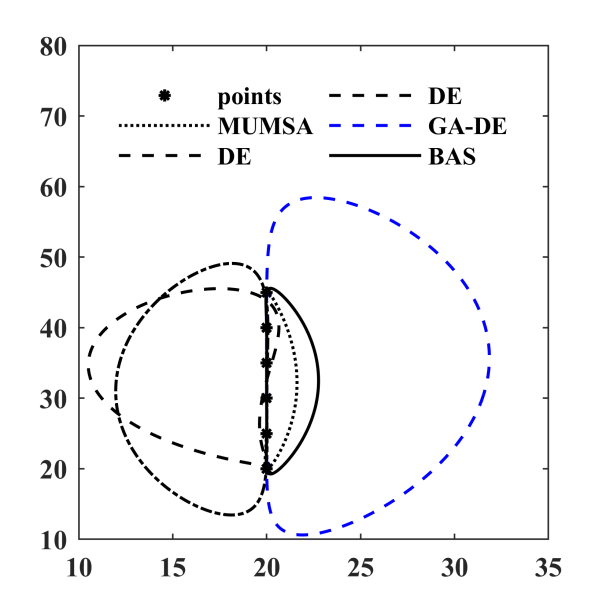
\includegraphics[width=0.5\linewidth]{img/case1png} 

}

\caption{各算法优化轨迹}\label{fig:case1png}
\end{figure}

\begin{table}

\caption{\label{tab:case1table}case1各算法结果对比}
\centering
\begin{tabular}[t]{lrrrrr}
\toprule
  & MUMSA & GA & DE & GA.DE & BAS\\
\midrule
\$r\_1\$ & 31.788264 & 28.771330 & 35.020740 & 13.2516000 & 19.4920810\\
\$r\_2\$ & 8.204647 & 5.000000 & 6.404196 & 5.9407800 & 6.2644716\\
\$r\_3\$ & 24.932131 & 35.365480 & 31.607220 & 58.3118000 & 20.1001631\\
\$r\_4\$ & 31.385926 & 59.136810 & 50.599490 & 53.7207000 & 19.0219161\\
\$r\_p\$ & 37.108246 & 14.850370 & 46.461261 & 61.3011560 & 39.8538048\\
\addlinespace
\$θ\_p\$ & 0.398977 & 1.570796 & 1.106544 & -1.3002600 & 0.3679660\\
\$θ\_0\$ & 4.015959 & 5.287474 & 0.000000 & 0.1960760 & 4.4245619\\
\$x\_0\$ & -6.366519 & 29.913290 & 60.000000 & -35.3621000 & -13.0300715\\
\$y\_0\$ & 56.836760 & 32.602280 & 18.077910 & 36.7704000 & 51.1796666\\
\$θ\_2\textasciicircum{}1\$ & 1.366547 & 6.283185 & 6.283185 & 1.6601500 & 5.9699819\\
\addlinespace
\$θ\_2\textasciicircum{}2\$ & 2.330773 & 0.318205 & 0.264935 & 2.0468400 & 0.4554995\\
\$θ\_2\textasciicircum{}3\$ & 2.871039 & 0.638520 & 0.500377 & 2.4281100 & 1.0202707\\
\$θ\_2\textasciicircum{}4\$ & 3.394591 & 0.979950 & 0.735321 & 2.8090100 & 1.5550696\\
\$θ\_2\textasciicircum{}5\$ & 3.970960 & 1.412732 & 0.996529 & 3.1900900 & 2.1117409\\
\$θ\_2\textasciicircum{}6\$ & 4.963490 & 2.076254 & 1.333549 & 3.5737900 & 2.8839248\\
\$Error\$ & 0.002057 & 1.101697 & 0.122738 & 0.0000172 & 0.0000124\\
\bottomrule
\end{tabular}
\end{table}

\subsection{Case2 有规定时间的轨迹生成(with prescribed
timing)}\label{case2-with-prescribed-timing}

本案例四杆机构的路径为5个没有对齐的点(规定时间)。通过式\eqref{eq:optim4bars}计算得到误差。

设计参数为:

\[
X = [r_1,r_2,r_3,r_4,r_p,\theta_p]
\] 目标点坐标:

\begin{align}
&\{C_d^i\} = \{(3,3),(2.759,3.363),(2.759,3.363),(1.890,3.862),(1.355,3.943)\} \notag \\
&\{\theta_2^1,\theta_2^2,\theta_2^3,\theta_2^4,\theta_2^5\}=\{\pi/6,\pi/4,\pi/3,5\pi/12,\pi/2\} \notag \\
\end{align}

参数约束:

\[
r_1,r_2,r_3,r_4\in[0,5]\quad r_p\in[-5,5]\quad \theta_p\in[0,2\pi]
\]

算法参数为
\(d_0 = 0.10,\delta_0=0.05,c_1=0.9998,c_2=0.5,q=40,T_{max}=10000\),动画结果如图\ref{fig:case2gif}。

\url{img/case2.gif}

与其他算法对比结果如图\ref{fig:case2png}和表\ref{tab:case2table}。

\begin{figure}

{\centering 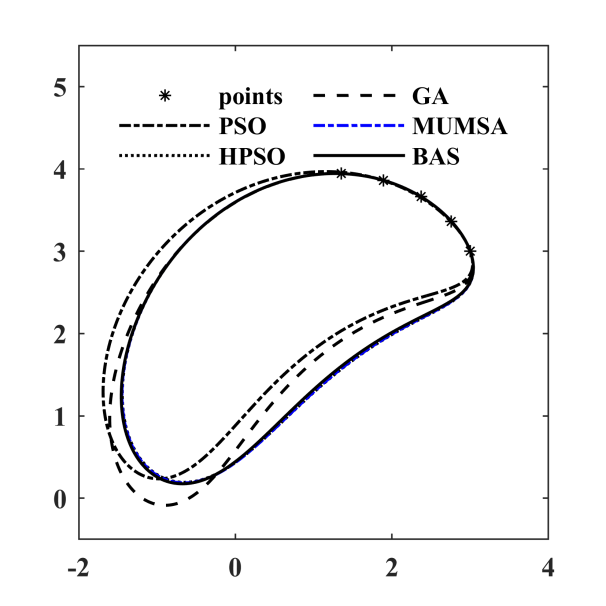
\includegraphics[width=0.5\linewidth]{img/case2png} 

}

\caption{各算法优化轨迹}\label{fig:case2png}
\end{figure}

\begin{table}

\caption{\label{tab:case2table}case2各算法结果对比}
\centering
\begin{tabular}[t]{lrrrrr}
\toprule
  & PSO & HPSO & GA & MUMSA & BAS\\
\midrule
\$r\_1\$ & 3.0576200 & 3.7877200 & 3.0630424 & 3.7732686 & 3.7135255\\
\$r\_2\$ & 1.8618400 & 1.9984200 & 1.9959624 & 2.0000040 & 1.9978745\\
\$r\_3\$ & 3.8459100 & 4.1331300 & 3.3058230 & 4.1169710 & 4.0469527\\
\$r\_4\$ & 2.9706300 & 2.7451300 & 2.5247060 & 2.7461567 & 2.7192391\\
\$r\_p\$ & 2.4968270 & 2.3697220 & 2.3721479 & 2.3684374 & 2.3702974\\
\addlinespace
\$θ\_p\$ & 0.7243557 & 0.7841479 & 0.8044176 & 0.7831567 & 0.7865371\\
\$Error\$ & 0.0005860 & 0.0009860 & 0.0000018 & 0.0000018 & 0.0000007\\
\bottomrule
\end{tabular}
\end{table}

\subsection{Case3 规定时间内路径生成(Path generation with prescribed
timing)}\label{case3-path-generation-with-prescribed-timing}

本案例四杆机构需要在规定时间通过一个闭环。通过式\eqref{eq:optim4bars}计算得到误差。

设计参数为:

\[
X = [r_1,r_2,r_3,r_4,r_p,\theta_p,\theta_0,x_0,y_0,\theta_2^1,\cdots,\theta_2^6]
\]

目标点坐标:

\begin{align}
\{C_d^i\} = \{&(0.5,1.1),(0.4,1.1),(0.3,1.1),(0.2,1.0),(0.1,0.9),(0.05,0.75), \notag \\
&(0.02,0.6),(0,0.5),(0,0.4),(0.03,0.3),(0.1,0.25),(0.15,0.2), \notag\\
&(0.2,0.3),(0.3,0.4),(0.4,0.5),(0.5,0.7),(0.6,0.9),(0.6,1.0)\} \notag\\
\{\theta_2^i\}=\{&\theta_2^1,\theta_2^1+20\cdot i/\pi\},\quad i = 1,\cdots,17 \notag \\
\end{align}

参数约束:

\[
r_1,r_2,r_3,r_4\in[0,5]\quad r_p,x_0,y_0\in[-5,5]\quad \theta_0,\theta_2^1,\theta_p\in[0,2\pi]
\]

算法参数为
\(d_0 = 0.10,\delta_0=0.05,c_1=0.9998,c_2=0.5,q=8,T_{max}=50000\),动画结果如图\ref{fig:case3gif}。

\url{img/case3.gif}

与其他算法对比结果如图\ref{fig:case3png}和表\ref{tab:case3table}。

\begin{figure}

{\centering 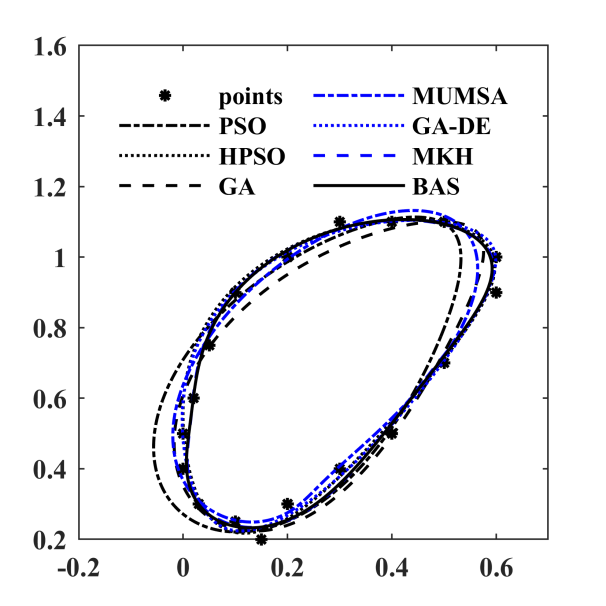
\includegraphics[width=0.5\linewidth]{img/case3png} 

}

\caption{各算法优化轨迹}\label{fig:case3png}
\end{figure}

\begin{table}

\caption{\label{tab:case3table}case3各算法结果对比}
\centering
\begin{tabular}[t]{lrrrrrrr}
\toprule
  & PSO & HPSO & GA & MUMSA & GA.DE & MKH & BAS\\
\midrule
\$r\_1\$ & 2.926100 & 2.850000 & 3.057878 & 4.453772 & 47.4379000 & 1.0042900 & 1.0541803\\
\$r\_2\$ & 0.487700 & 0.370000 & 0.237803 & 0.297057 & 0.3247700 & 0.4218000 & 0.4238711\\
\$r\_3\$ & 2.909900 & 2.904800 & 4.828954 & 3.913095 & 0.4728570 & 0.8782100 & 0.9145640\\
\$r\_4\$ & 2.150300 & 0.500000 & 2.056465 & 0.849372 & 47.3093000 & 0.5801300 & 0.5988706\\
\$r\_p\$ & 1.493947 & 1.973700 & 2.003475 & 2.651983 & 0.3412513 & 0.5234000 & 0.5450268\\
\addlinespace
\$θ\_p\$ & -0.332546 & 1.027396 & 1.177913 & 2.464734 & -1.2153827 & 0.8147728 & 0.8227469\\
\$θ\_0\$ & 0.719000 & 0.760000 & 1.002168 & 2.738736 & 3.3202900 & 0.2929400 & 0.2850398\\
\$x\_0\$ & -0.384600 & 0.940000 & 1.776808 & -1.309243 & 0.5269880 & 0.2688600 & 0.2676998\\
\$y\_0\$ & -0.675200 & -1.171200 & -0.641991 & 2.806964 & 0.7239300 & 0.1771500 & 0.1544272\\
\$θ\_2\textasciicircum{}1\$ & 0.215900 & 0.513400 & 0.226186 & 4.853543 & 3.5123300 & 0.8859500 & 1.1764113\\
\$Error\$ & 0.049200 & 0.011100 & 0.033700 & 0.019600 & 0.0108613 & 0.0091100 & 0.0090289\\
\bottomrule
\end{tabular}
\end{table}

\subsection{Case4 规定时间路径生成问题}\label{case4-}

第四个案例同样是一个规定时间的路径生成问题。六个优化点由一个\texttt{semi-archer}弧构成,问题定义如下。

设计参数为:

\[
X = [r_1,r_2,r_3,r_4,r_p,\theta_p,\theta_0,x_0,y_0]
\]

目标点坐标:

\begin{align}
&\{C_d^i\} = \{(0,0),(1.9098,5.8779),(6.60989.5106),(13.09,9.5106),(18.09,5.8779),(20,0)\} \notag \\
&\{\theta_2^1,\theta_2^2,\theta_2^3,\theta_2^4,\theta_2^5\}=\{\pi/6,\pi/3,\pi/2,2\pi/3,5\pi/6,\pi\} \notag \\
\end{align}

参数约束:

\[
r_1,r_2,r_3,r_4\in[0,50]\quad r_p,x_0,y_0\in[-50,50]\quad \theta_0,\theta_p\in[0,2\pi]
\]

算法参数为
\(d_0 = 0.10,\delta_0=0.05,c_1=0.9997,c_2=0.5,q=40,T_{max}=30000\),动画结果如图\ref{fig:case4gif}。

\url{img/case4.gif}

与其他算法对比结果如图\ref{fig:case4png}和表\ref{tab:case4table}。

\begin{figure}

{\centering 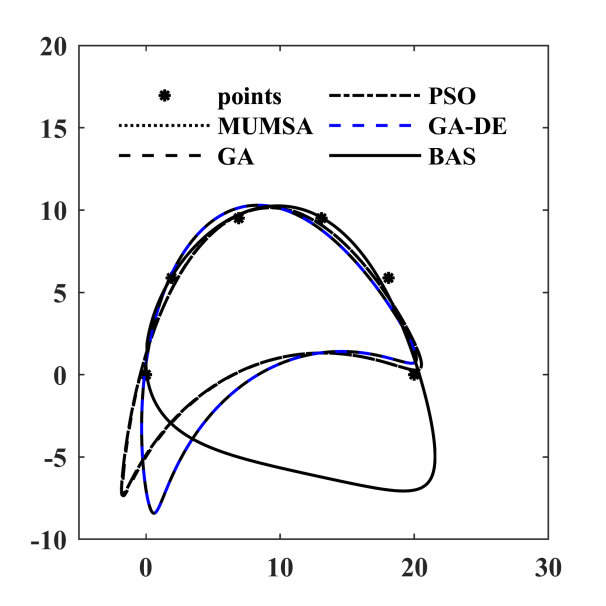
\includegraphics[width=0.5\linewidth]{img/case4png} 

}

\caption{各算法优化轨迹}\label{fig:case4png}
\end{figure}

\begin{table}

\caption{\label{tab:case4table}case4各算法结果对比}
\centering
\begin{tabular}[t]{lrrrrr}
\toprule
  & MUMSA & GA & PSO & GA.DE & BAS\\
\midrule
\$r\_1\$ & 50.0000000 & 50.0000000 & 50.0000000 & 50.000000 & 47.2345017\\
\$r\_2\$ & 5.0000000 & 5.0000000 & 5.0000000 & 5.000000 & 8.8473992\\
\$r\_3\$ & 7.0310470 & 6.9700900 & 7.0310200 & 5.905343 & 25.0474709\\
\$r\_4\$ & 48.1341830 & 48.1993000 & 48.1342000 & 50.000000 & 50.0000000\\
\$r\_p\$ & 21.3533558 & 21.2191204 & 21.3532819 & 18.819312 & 50.0000000\\
\addlinespace
\$θ\_p\$ & 0.6517294 & 0.6380060 & 0.6517238 & 0.000000 & 5.7107187\\
\$θ\_0\$ & 0.0428247 & 0.0508453 & 0.0428286 & 0.463633 & 0.8225945\\
\$x\_0\$ & 12.1974940 & 12.2377000 & 12.1975000 & 14.373772 & 16.5531171\\
\$y\_0\$ & -15.9982030 & -15.8332000 & -15.9981000 & -12.444295 & -48.1473786\\
\$Error\$ & 2.5803500 & 2.5828600 & 2.5803600 & 2.349649 & 0.7863680\\
\bottomrule
\end{tabular}
\end{table}

\subsection{Case5 规定时间内路径生成问题}\label{case5-}

这个例子是一个椭圆路径生成问题,没有规定的时间,其中轨迹是由10个点定义的。问题定义如下。

设计参数为:

\[
X = [r_1,r_2,r_3,r_4,r_p,\theta_p,\theta_0,x_0,y_0,\theta_2^1,\cdots,\theta_2^{10}]
\]

目标点坐标:

\begin{align}
\{C_d^i\} = \{&(20,10),(17.66,15.142),(11.736,17.878),(5,16.928),(0.60307,12.736), \notag \\
&(0.60307,7.2638),(5,3.0718),(11.736,2.1215),(17.66,4.8577),(20,0)\}\notag\\
\end{align}

参数约束:

\[
r_1,r_2,r_3,r_4\in[0,80]\quad r_p,x_0,y_0\in[-80,80]\quad \theta_0,\theta_2^1,\cdots,\theta_2^{10},\theta_p\in[0,2\pi]
\]

算法参数为
\(d_0 = 0.10,\delta_0=0.05,c_1=0.9998,c_2=0.5,q=40,T_{max}=40000\),动画结果如图\ref{fig:case5gif}。

\url{img/case5.gif}

与其他算法对比结果如图\ref{fig:case5png}和表\ref{tab:case5table}。

\begin{figure}

{\centering 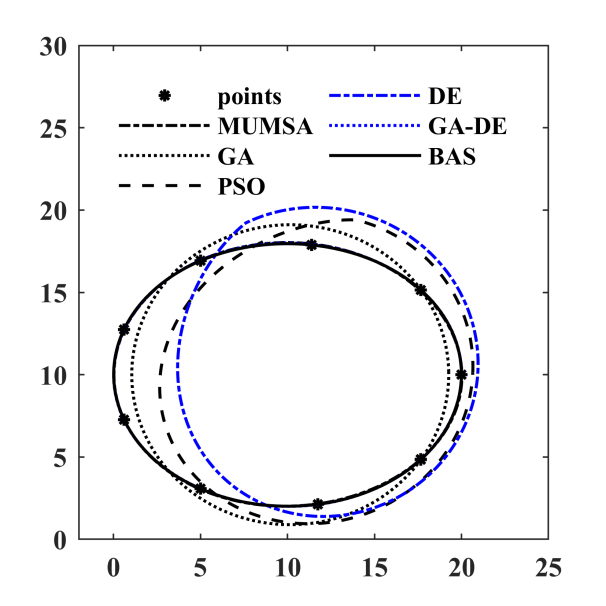
\includegraphics[width=0.5\linewidth]{img/case5png} 

}

\caption{各算法优化轨迹}\label{fig:case5png}
\end{figure}

\begin{table}

\caption{\label{tab:case5table}case5各算法结果对比}
\centering
\begin{tabular}[t]{lrrrrrr}
\toprule
  & MUMSA & GA & PSO & DE & GA.DE & BAS\\
\midrule
\$r\_1\$ & 79.5160680 & 79.981513 & 52.535162 & 54.360893 & 80.0000000 & 71.8681225\\
\$r\_2\$ & 9.7239730 & 9.109993 & 8.687886 & 8.683351 & 8.4203200 & 9.2618623\\
\$r\_3\$ & 45.8425240 & 72.936511 & 36.155078 & 34.318634 & 51.3426000 & 44.4542963\\
\$r\_4\$ & 51.4384800 & 80.000000 & 80.000000 & 79.996171 & 42.4532000 & 43.0533508\\
\$r\_p\$ & 8.7289390 & 0.000000 & 1.481055 & 1.465250 & 10.6530404 & 8.7820722\\
\addlinespace
\$θ\_p\$ & -0.3452264 & 0.000000 & 1.570796 & 1.570669 & 2.6465448 & 1.6362575\\
\$θ\_0\$ & 5.5969445 & 0.026149 & 1.403504 & 2.129650 & 4.2817700 & 1.6011655\\
\$x\_0\$ & 2.0211090 & 10.155966 & 11.002124 & 10.954397 & 5.5337200 & 16.7540360\\
\$y\_0\$ & 13.2165878 & 10.000000 & 11.095585 & 11.074534 & 0.4771830 & 15.2986682\\
\$θ\_2\textasciicircum{}1\$ & 0.6376873 & 6.283185 & 6.282619 & 6.283185 & 2.0935000 & 0.1258416\\
\addlinespace
\$θ\_2\textasciicircum{}2\$ & 1.3255329 & 0.600745 & 0.615302 & 0.616731 & 2.8129100 & 0.8167208\\
\$θ\_2\textasciicircum{}3\$ & 2.0080339 & 1.372812 & 1.305421 & 1.310254 & 3.5160500 & 1.5351326\\
\$θ\_2\textasciicircum{}4\$ & 2.6955659 & 2.210575 & 2.188053 & 2.193570 & 4.2063800 & 2.1811489\\
\$θ\_2\textasciicircum{}5\$ & 3.3845794 & 2.862639 & 2.913049 & 2.917170 & 4.8905100 & 2.8753839\\
\$θ\_2\textasciicircum{}6\$ & 4.0829376 & 3.420547 & 3.499313 & 3.490746 & 5.5739800 & 3.5728072\\
\addlinespace
\$θ\_2\textasciicircum{}7\$ & 4.7984548 & 4.072611 & 4.125586 & 4.132017 & 6.2645800 & 4.2854058\\
\$θ\_2\textasciicircum{}8\$ & 5.5117056 & 4.910373 & 4.919977 & 4.922075 & 0.6761980 & 5.0016208\\
\$θ\_2\textasciicircum{}9\$ & 6.2127919 & 5.682440 & 5.685021 & 5.695372 & 1.3830700 & 5.7133417\\
\$θ\_2\textasciicircum{}\{10\}\$ & 0.6371866 & 6.283185 & 6.282323 & 6.282970 & 2.0934800 & 0.1258290\\
\$Error\$ & 0.0047000 & 2.281273 & 1.971004 & 1.952326 & 0.0006022 & 0.0004252\\
\bottomrule
\end{tabular}
\end{table}

\subsection{Case6 六杆机构路径生成}\label{case6-}

这个案例我也看不懂。大概意思是,六杆问题,在规定时间内让轨迹耦合目标点,并且\texttt{output\ link}在停顿位置(\texttt{dwell\ portion}?我翻译不下去了\ldots{}\ldots{})保持在一个精确的角度。大家看底下的原文靠谱一点。

\begin{quote}
``This case is a path and function combined synthesis problem with
prescribed timing in which the coupler of six-bar mechanism has to the
precision points and its output link has to maintain an accuracy angle
in the dwell portion.''

\begin{flushright}--- Xiaojuan Mo\end{flushright}
\end{quote}

设计参数为:

\[
X = [r_1,r_2,r_3,r_4,r_5,r_6,r_p,\theta_p,r_1',\theta_0,\theta_0',x_0,y_0,\theta_2^1] 
\]

目标点坐标:

\begin{align}
\{C_d^i\} = \{&(-0.5424,2.3708),(0.2202,2.9871),(0.9761,3.4633), \notag \\
&(1.0618,36380),(0.8835,3.7226),(0.5629,3.7156),\notag \\
&(0.1744,3.6128),(-0.2338,3.4206),(-0.6315,3.1536), \notag \\
&(-1.0,2.8284),(-1.3251,2.4600),(-1.5922,2.0622), \notag \\
&(-1.7844,1.6539),(-1.8872,1.2654),(-1.8942,0.9448), \notag \\
&(-1.8096,0.7665),(-1.6349,0.8522),(-1.1587,1.6081)\} \notag \\
\{\theta_2^i\} = \{&0,15,40,60,80,100,120,140,160,180,\notag \\
& 200, 220,240,260,280,300,320,345\} \notag \\
& \rightarrow \theta_2^i = \theta_2 + \delta_2^i \notag \\
\end{align}

在停顿位置处的输入输出角度的关联如下:

\begin{align}
&\theta_2^i = \theta_2^1+\{160,180,200,220\}\rightarrow \theta_6^i=210 \notag \\
&\theta_2^i=\theta_2^1+\{345,0,15\} \rightarrow \theta_6^i = 225 \notag \\
\end{align}

\begin{quote}
注意,上述涉及到角度的数值单位均为deg,而非弧度。
\end{quote}

算法参数为
\(d_0 = 0.05,\delta_0=0.025,c_1=0.9999,c_2=0.5,q=10,T_{max}=50000\),动画结果如图\ref{fig:case6gif}。

\url{img/case6.gif}

与其他算法对比结果如图\ref{fig:case6png},
图\ref{fig:case6png2}和表\ref{tab:case6table}。

\begin{figure}

{\centering 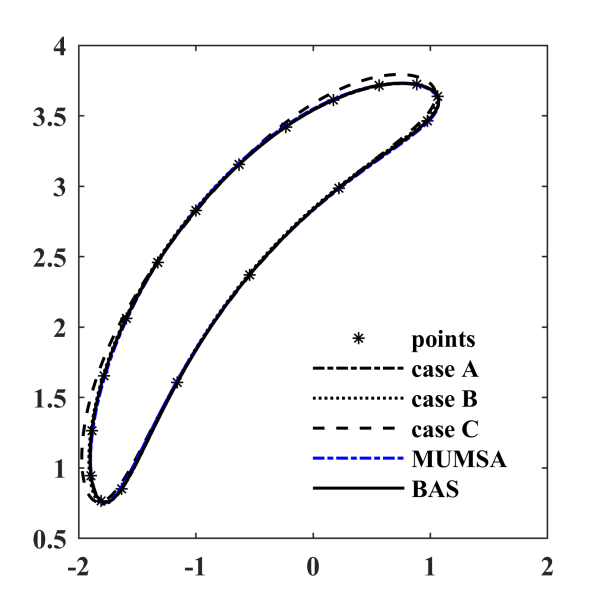
\includegraphics[width=0.5\linewidth]{img/case6png} 

}

\caption{各算法优化轨迹}\label{fig:case6png}
\end{figure}

\begin{figure}

{\centering 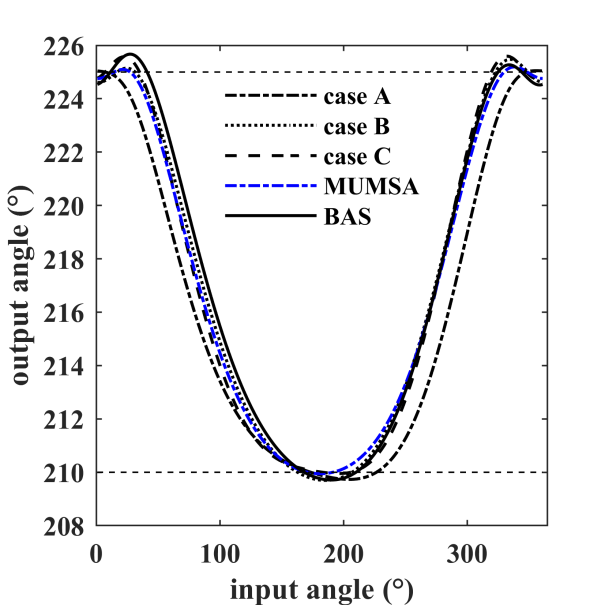
\includegraphics[width=0.5\linewidth]{img/case6png2} 

}

\caption{各算法优化角度}\label{fig:case6png2}
\end{figure}

\begin{table}

\caption{\label{tab:case6table}case6各算法结果对比}
\centering
\begin{tabular}[t]{llllll}
\toprule
  & DE.A & DE.B & DE.C & MUMSA & BAS\\
\midrule
\$r\_1\$ & 1.8145 & 1.8065 & 2.0926 & 1.713529 & 1.838058488\\
\$r\_2\$ & 0.9911 & 0.9826 & 1.1464 & 0.92602 & 1.006097698\\
\$r\_3\$ & 1.9995 & 2.0177 & 1.989 & 1.991373 & 1.997800646\\
\$r\_4\$ & 2.0315 & 2.0009 & 1.9727 & 1.848672 & 2.008472163\\
\$r\_5\$ & 4.3674 & 5.7769 & 6.6633 & 5.35498 & 6.106586728\\
\addlinespace
\$r\_6\$ & 2.4924 & 2.5296 & 2.5517 & 2.54979 & 2.551492193\\
\$r\_p\$ & 2.8174 & 2.8711 & 2.7178 & 2.975936132 & 2.815041279\\
\$θ\_p\$ & 0.7776 & 0.783712 & 0.845246 & 0.831651258 & 0.78386985\\
\$θ\_0\$ & 6.269879 & 0.011582 & 6.242260827 & 0.067677 & 6.277427755\\
\$r\_1'\$ & 4.4158 & 5.2817 & 6.2907 & 4.87374 & 5.63828226\\
\addlinespace
\$θ\_0'\$ & 0.235595 & 0.0170309 & 6.18118303 & 0.0967027 & 6.257863894\\
\$x\_0\$ & 0.0115 & 0.0415 & -0.2729 & 0.175257 & -0.013849346\\
\$y\_0\$ & 0.0157 & -0.0377 & 0.0931 & -0.1187032 & 0.011591976\\
\$θ\_2\textasciicircum{}1\$ & 0.00052 & 0.003648 & -0.04062 & 6.222361 & 6.281768246\\
\$Evaluations\$ & 53310 & 93405 & 93405 & 93405 & 50000\\
\$Error\$ & 0.000250876 & 0.005653158 & 0.03537533 & 0.0014 & 0.000195212659\\
\bottomrule
\end{tabular}
\end{table}

\subsection{Case7 无规定时间的路径生成}\label{case7-}

本案例为一个'8'型路径生成问题,轨迹由12个点规定。

设计参数为:

\[
X = [r_1,r_2,r_3,r_4,r_p,\theta_p,\theta_0,x_0,y_0,\theta_2^1,\cdots,\theta_2^{12}]
\]

目标点坐标:

\begin{align}
\{C_d^i\} = \{&(4.15,2.21),(4.50,2.18),(4.53,1.83),(4.13,1.68),(3.67,1.58),(2.96,1.33), \notag \\
&(2.67,1.06),(2.63,0.82),(2.92,0.81),(3.23,1.07),(3.49,1.45),(3.76,1.87)\}\notag\\
\end{align}

参数约束:

\begin{align}
&r_1\in[0,5]\quad r_2,r_3,r_4\in[0,10] \quad r_p\in[0,14],\notag \\
&x_0,y_0\in[-80,80]\quad \theta_0,\theta_2^1,\cdots,\theta_2^{12},\theta_p\in[0,2\pi] \notag \\
\end{align}

算法参数为
\(d_0 = 0.05,\delta_0=0.025,c_1=0.9995,c_2=0.5,q=40,T_{max}=20000\),动画结果如图\ref{fig:case7gif}。

\url{img/case7.gif}

与其他算法对比结果如图\ref{fig:case7png}和表\ref{tab:case7table}。

\begin{figure}

{\centering 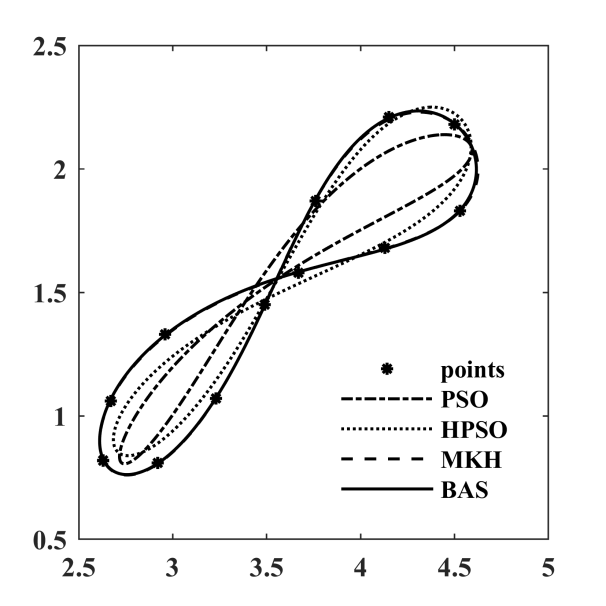
\includegraphics[width=0.5\linewidth]{img/case7png} 

}

\caption{各算法优化轨迹}\label{fig:case7png}
\end{figure}

\begin{table}

\caption{\label{tab:case7table}case7各算法结果对比}
\centering
\begin{tabular}[t]{lrrrr}
\toprule
  & PSO & HPSO & MKH & BAS\\
\midrule
\$r\_1\$ & 4.550300 & 4.535900 & 2.8764500 & 2.8162769\\
\$r\_2\$ & 1.101300 & 1.113300 & 1.1464400 & 1.1382629\\
\$r\_3\$ & 3.955800 & 14.738100 & 4.4077300 & 4.0509922\\
\$r\_4\$ & 3.933000 & 16.801700 & 4.7571300 & 4.1957758\\
\$r\_p\$ & 3.941572 & 3.941866 & 2.6665746 & 2.6682801\\
\addlinespace
\$θ\_p\$ & -0.539171 & -1.521104 & -1.1363513 & 5.1910788\\
\$θ\_0\$ & 0.000000 & 0.000000 & 0.1650200 & 0.2070603\\
\$x\_0\$ & 0.000000 & 0.000000 & 1.1426500 & 1.1226995\\
\$y\_0\$ & 0.000000 & 0.000000 & 0.4823700 & 0.5246662\\
\$θ\_2\textasciicircum{}1\$ & -0.201400 & -0.181600 & -0.3139900 & 6.1191060\\
\$Error\$ & 0.171600 & 0.096400 & 0.0001597 & 0.0000994\\
\bottomrule
\end{tabular}
\end{table}

\subsection{Case8 无规定时间的路径生成}\label{case8-}

本案例为一个叶形路径生成问题(无规定时间),轨迹由25个点规定。

设计参数为:

\[
X = [r_1,r_2,r_3,r_4,r_p,\theta_p,\theta_0,x_0,y_0,\theta_2^1,\cdots,\theta_2^{25}]
\]

目标点坐标:

\begin{align}
\{C_d^i\} = \{&(7.03,5.99),(6.95,5.45),(6.77,5.03),(6.4,4.6),(5.91,4.03), \notag \\
&(5.43,3.56),(4.93,2.94),(4.67,2.6),(4.38,2.2),(4.04,1.67),\notag \\
&(3.76,1.22),(3.76,1.97),(3.76,2.78),(3.76,3.56),(3.76,4.34), \notag \\
&(3.76,4.91),(3.76,5.47),(3.8,5.98),(4.07,6.4),(4.53,6.75), \notag \\
&(5.07,6.85),(5.05,6.84),(5.89,6.83),(6.41,6.8),(6.92,6.58)\} \notag \\
\end{align}

参数约束:

\[
r_1,r_2,r_3,r_4\in[0,5]\quad r_p,x_0,y_0\in[-5,5] \quad \theta_0,\theta_2^1,\cdots,\theta_2^{25},\theta_p\in[0,2\pi]
\]

算法参数为
\(d_0 = 0.05,\delta_0=0.025,c_1=0.99975,c_2=0.5,q=40,T_{max}=50000\),动画结果如图\ref{fig:case8gif}。

\url{img/case8.gif}

与其他算法对比结果如图\ref{fig:case8png}和表\ref{tab:case8table}。

\begin{figure}

{\centering 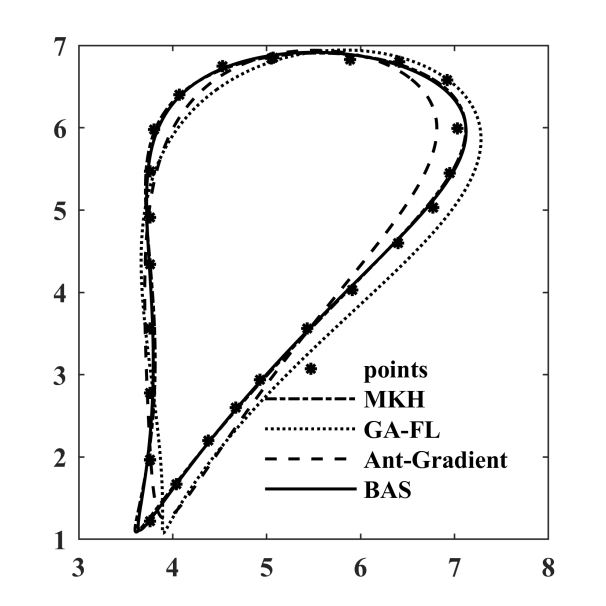
\includegraphics[width=0.5\linewidth]{img/case8png} 

}

\caption{各算法优化轨迹}\label{fig:case8png}
\end{figure}

\begin{table}

\caption{\label{tab:case8table}case8各算法结果对比}
\centering
\begin{tabular}[t]{llllr}
\toprule
  & MKH & GA.FL & Ant.Gradient & BAS\\
\midrule
\$r\_1\$ & 9.99432 & 9 & 13.08 & 9.6132193\\
\$r\_2\$ & 1.93027 & 3.01 & 1.89 & 1.9459840\\
\$r\_3\$ & 4.57242 & 8.8 & 8.41 & 4.9080817\\
\$r\_4\$ & 7.36674 & 8.8 & 6.75 & 6.6768279\\
\$r\_p\$ & 8.04254 & 11.0995 & 14.45 & 8.6409226\\
\addlinespace
\$θ\_p\$ & 0.187430 & -0.681 & 0.195 & 0.1694076\\
\$θ\_0\$ & -0.61763 & 0.489 & -0.3815 & 5.7260733\\
\$x\_0\$ & -2.31301 & -2.4 & -8.77 & -2.9214626\\
\$y\_0\$ & 2.86189 & -4 & 1.20 & 2.7190256\\
\$θ\_2\textasciicircum{}1\$ & * & * & * & 0.4529787\\
\$Error\$ & 0.03916 & 0.9022 & 0.5504 & 0.0397777\\
\bottomrule
\end{tabular}
\end{table}

\chapter{更新及维护计划}\label{updates}

\section{待加入的功能}

算法:

\begin{itemize}
\tightlist
\item
  \sout{加入\texttt{BSAS}}
\item
  \sout{加入\texttt{BSAS-WPT}}
\item
  加入\texttt{binary\ BAS} (阮月)
\item
  加入二阶 \texttt{BAS} (李晓晓)
\item
  add \texttt{BSO(Beetle\ Swarm\ Optimizaiton)} (王甜甜)
\item
  \ldots{}
\end{itemize}

应用:

\begin{itemize}
\tightlist
\item
  工程应用:

  \begin{itemize}
  \tightlist
  \item
    \sout{多杆件机构优化}(莫小娟)
  \item
    建筑系统阻容模型辨识
  \item
    装配路径规划
  \item
    批量问题(binary BAS)
  \item
    \ldots{}
  \end{itemize}
\item
  基准测试

  \begin{itemize}
  \tightlist
  \item
    计划超过20个基准测试
  \item
    \ldots{}
  \end{itemize}
\end{itemize}

用户界面:

\begin{itemize}
\tightlist
\item
  基本界面

  \begin{itemize}
  \tightlist
  \item
    \sout{基本的\texttt{shiny}界面}
  \item
    \sout{更新了约束处理功能}
  \item
    \ldots{}
  \end{itemize}
\item
  自动文档

  \begin{itemize}
  \tightlist
  \item
    基于\href{https://github.com/rstudio/rmarkdown}{rmarkdown}的自动文档报告生成
  \item
    文档导出
  \item
    \ldots{}
  \end{itemize}
\end{itemize}

算法部分与用户界面将会在\texttt{rBAS}包中不断更新。应用方面虽然有计划,但是除却基准测试外,更多的需要各位同学们的贡献。这部分暂时会选择几个重要的应用集成在\texttt{rBAS}包的案例库中,全部内容则会在本手册中更新。

\section{联系方式}

\begin{enumerate}
\def\labelenumi{\arabic{enumi}.}
\item
  大家可以加入QQ群(437958608)来讨论涉及\texttt{BAS}算法的各种问题。
\item
  更进一步,如果大家有意愿将自己的研究纳入\texttt{rBAS}包或者是手册的应用案例上,欢迎大家给我发送邮件(\texttt{jywang2016@hust.edu.cn})或者群内私信。具体的代码(如果大家愿意开源的话)或者文档形式(没有代码也是十分欢迎的)都可以具体商议。我也会尽量尝试将大家的\texttt{matlab}或者\texttt{python}代码复现为\texttt{R},所以``语言阻碍''暂时还不是问题。
\item
  如果对\texttt{rBAS}有什么建议,或者\texttt{bugs},欢迎大家在\href{https://github.com/jywang2016/rBAS/issues}{issues}上发表评论。
\end{enumerate}

\cleardoublepage 

\appendix \addcontentsline{toc}{chapter}{\appendixname}


\chapter*{结语}


暂无

\bibliography{book.bib,packages.bib,article.bib}

\backmatter
\printindex

\end{document}
